\documentclass[oneside]{template/openetcs_report}
% Use the option "nocc" if the document is not licensed under Creative Commons
%\documentclass[nocc]{template/openetcs_article}
\usepackage{lipsum,url}
\usepackage{supertabular}
\usepackage{longtable,tabu,booktabs}
\usepackage{graphicx}
\usepackage{multirow}
\usepackage{color, colortbl}
\usepackage[colorlinks=true, linkcolor=blue, urlcolor=blue,filecolor=blue]{hyperref}
\usepackage{listings}
\usepackage{makeidx}
\definecolor{gray}{rgb}{0.8,0.8,0.8}
\usepackage{lineno}
\usepackage{float}
\usepackage[color=green!40,textsize=footnotesize,textwidth=2.8cm]{todonotes}
%\usepackage{pdflscape}
%\usepackage[acronym, % list of acronyms
  %section, % add the glossary to the table of content
            %description,% acronyms have a user-supplied description,
 %style=longheader, % table style
 %nonumberlist % no page number
 %]{glossaries}
 
% make lists more compact with enumitem package (spacings below are set globally)
\usepackage{enumitem}
\setlist[description]{itemsep=1ex,topsep=1ex,partopsep=0.0ex,parsep=0.0ex}
\setlist[itemize]{itemsep=1ex,topsep=1ex,partopsep=0.0ex,parsep=0.0ex}
\setlist[enumerate]{itemsep=1ex,topsep=1ex,partopsep=0.0ex,parsep=0.0ex}

\graphicspath{{./template/}{.}{./images/}}

%\renewcommand*{\glspostdescription}{} %Deactivate point at the end of every description
%\renewcommand*{\glossaryname}{Glossary}

%create glossary
% \makeglossaries
 %Glossary terms
% \loadglsentries{glossary}

\begin{document}
\frontmatter
\project{openETCS}

\newcommand{\define}[1]{\index{#1}\emph{#1}}



%Please do not change anything above this line
%============================

% The document metadata is defined below

%assign a report number here
\reportnum{OETCS/WP3/D3.5.3}

%define your workpackage here
\wp{Work Package 3: ``Modeling''}

%set a title here
\title{openETCS Architecture and Design Specification}

%set a subtitle here
\subtitle{Software Component Design and Internal Interface Specification}

%set the date of the report here
\date{September 2015}


%document approval
%define the name and affiliation of the people involved in the documents approbation here
\creatorname{Peter Mahlmann}
\creatoraffil{DB Netz AG}

\techassessorname{Jan Welte}
\techassessoraffil{Technische Universität Braunschweig}

\qualityassessorname{Marc Behrens}
\qualityassessoraffil{DLR}

\approvalname{Klaus-R\"udiger Hase}
\approvalaffil{DB Netz AG}


%define a list of authors and their affiliation here

\author{Peter Mahlmann, Bernd Hekele, Baseliyos Jacob, Peyman Farhangi}
\affiliation{DB Netz AG}

\author{Uwe Steinke}
\affiliation{Siemens AG}

\author{Christian Stahl}
\affiliation{TWT GmbH}

\author{Jakob G\"artner, Mairamou Haman Adji, Stefan Karg}
\affiliation{LEA Railergy}

%\author{Jos Holtzer, Jan Welvaarts, Vincent Nuhaan}
%\affiliation{Nederlandss Spoorwegen}

\author{Thorsten Schulz}
\affiliation{University of Rostock}

\author{Marielle Petit-Doche}
\affiliation{Systerel}

%\author{Veronique Gontier}
%\affiliation{All4Tec}

%\author{Christian Giraud, Fausto Cochetti}
%\affiliation{Alstom}

\author{Alexander Stante}
\affiliation{Fraunhofer ESK}

%\author{David Mentre}
%\affiliation{MERCE}




% define the coverart
\coverart[width=350pt]{openETCS_EUPL}

\newpage
%define the type of report
\reporttype{Architecture and Design Specification}


\begin{abstract}
%define an abstract here
This document describes the architecture and design specification of  the openETCS onboard unit (OBU) model. The functional scope of the openETCS OBU model is to cover the functionality required for running on the ETCS level $2$ Utrecht Amsterdam track. The OBU model is developed iteratively and the system model is documented in D3.5.x and the functional model is documented in D3.5.x, where x denotes the iteration. 
\end{abstract}

%=============================
\maketitle

%Modification history
%if you do not need a modification history table for your document simply comment out the eight lines below
%=============================


\chapter*{Modification History}
\tablefirsthead{
\toprule
%\rowcolor{gray} 
Version & Sections & Modification / Description & Author & Date \\\midrule}
\begin{supertabular}{ m{1.2cm}  m{1.5cm}  m{5.0cm}  m{3cm}  m{2.5cm} }
0.1 & all & Initial document providing structure & Peter Mahlmann& 27.05.2015 \\\midrule
0.2 & 2 & New template for design descriptions & Peter Mahlmann& 10.06.2015 \\\midrule
0.3 & all & Transferred existing documentation to new template & Peter Mahlmann& 22.06.2015\\\midrule
0.4 & 5 & Updated component hierarchy to match current SCADE model & Peter Mahlmann & 15.09.2015 \\\bottomrule

\end{supertabular}

% list subsubsections in table of contents
%\setcounter{tocdepth}{3}
\setcounter{secnumdepth}{3}   
\setcounter{tocdepth}{3}   

\pdfbookmark{\contentsname}{toc}
\tableofcontents
\listoffigures
\listoftodos
\newpage
%=============================

%Uncomment the next line if you need line numbers for tracebility when the document is in review
\linenumbers
%=============================


% The actual document starts below this line
%=============================


\mainmatter

\setlength{\topsep}{0.5ex}
\setlength{\itemsep}{0ex}
\setlength{\parsep}{0ex}

%set the master document for easy compilation
%!TEX root = ../D3_5_3.tex

\chapter{Introduction}

A primary goal of the openETCS ITEA2 project is to provide a formal specification and a non-vital reference implementation of an ETCS onboard unit (OBU) according to the specification defined in Subset-026 \cite{subset-026} by the European Railway Agency (ERA). 

This deliverable, i.e.~D3.5.x, describes the architecture and design specification of the openETCS onboard (OBU) model. As the development of the OBU model is done iteratively according to a SCRUM process, the last digit of the deliverable identifier, i.e.~x, denotes the current iteration of the model. This document should be considered as a complement to the following project outcomes respectively deliverables:
\begin{itemize}
\item the corresponding SysML model (SCADE System), available at \url{https://github.com/openETCS/modeling/tree/master/model/system},
\item the corresponding functional model (SCADE Suite), available at \url{https://github.com/openETCS/modeling/tree/master/model/Scade/System},
\item the corresponding functional design description, i.e.~D3.6.x, and
\item the documentation of the generic openETCS Application Programming Interface (API), available at \url{https://github.com/openETCS/modeling/blob/master/API/description/api-description.pdf}.
\todo[inline]{links need to be corrected, in particular links to the API documentation}
\end{itemize}


\section{Input Documents}

The following documents have been the basis for the analysis, functional decomposition, and design of the openETCS OBU model:
\begin{itemize}
\item ERA Subset-026 \cite{subset-026}, V3.3.0
\item ERA TSI CCS Documents
\item openETCS API documentation, available at \url{https://github.com/openETCS/modeling/blob/master/API/description/api-description.pdf}
\item openETCS requirements, i.e.~D2.1, D2.2,$\ldots$, D2.9, available at \url{https://github.com/openETCS/requirements/tree/master/Reference}
\todo[inline]{list has to be completed}
\end{itemize}


\section{Software and Tools used for Development}

The following software and tools have been used in the openETCS development process:
\todo[inline]{list and descriptions have to be checked for completeness}
\begin{description}
\item[SCADE System] Version 16.1b of SCADE System has been used for the the generation of SysML models.
\item[SCADE Suite] Version 16.1b of SCADE Suite has been used for the functional modelling of the openETCS OBU components. Executable models are generated via the SCADE Suite code generator (KCG), which has been certified for CENELEC EN 50128 at SIL 3/4.
\item[SCADE Display] Version 16.1b of SCADE Display has been used for the development of the Driver Machine Interface (DMI).
\item[GitHub] The web based Git repository hosting service GitHub has been used for distributed revision control and source code respectively model management.
\end{description}


\section{General Remarks on the openETCS OBU Model}
The openETCS OBU model has been developed according the specification given in ERA Subset-026 \cite{subset-026}, Version 3.3.0. The software release of the openETCS OBU documented and described in this document is publicly available at \url{https://github.com/openETCS/modeling/tree/master/model} and refers to the commit corresponding to the following hashtag:
\begin{quotation}
\centering
\todo[inline]{Hashtag has to be updated once the model and document are ready for release}
\texttt{1c06cc2d4a0d8f27569e065e2a9edf924b453ff1}
\end{quotation}
In particular, the root of the SysML model is located at
\url{https://github.com/openETCS/modeling/tree/master/model/system}
and the root of the functional SCADE Suite model is located at
\url{https://github.com/openETCS/modeling/tree/master/model/Scade}.

Note that all components of the openETCS OBU have been developed from scratch, no existing components have been reused.

\part{System Architecture and Functional Breakdown}

%%set the master document for easy compilation
%!TEX root = ../D3_5_2.tex

\chapter{openETCS API Runtime System and Input to the EVC)}
\label{chp_openETCS_API}
%Authors: Bernd Hekele (DB)

\begin{figure}[hbtp]
\centering
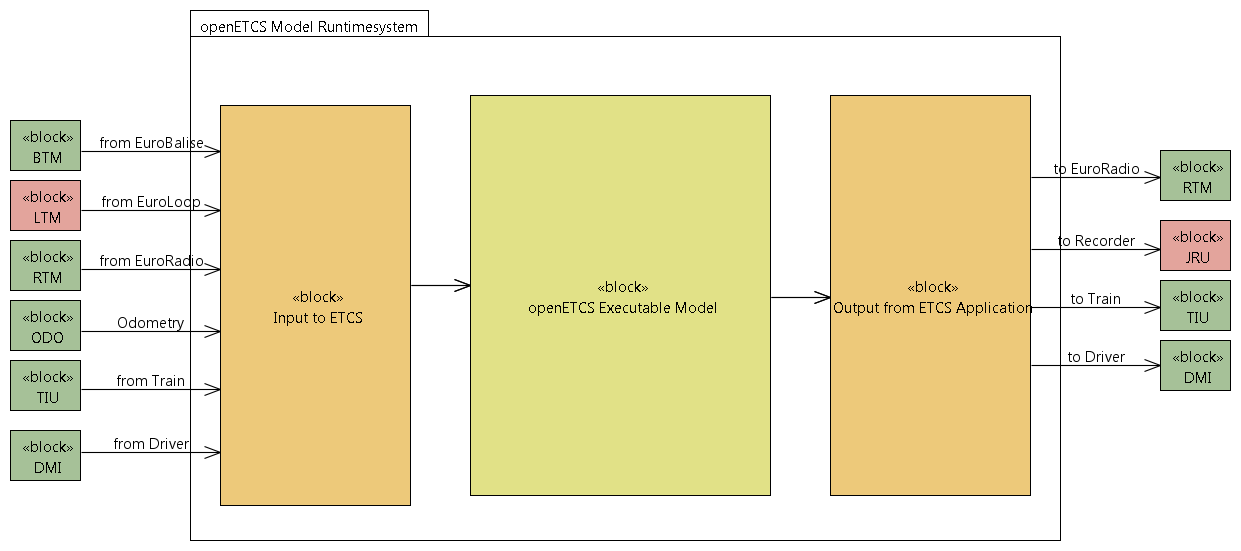
\includegraphics[width=\linewidth]{openETCSAPI.png}
\caption{openETCS API Highlevel View}
\label{fig:apiHighLevel}
\end{figure}

Figure \ref{fig:apiHighLevel} shows the structure of API with respect to the software architecture. Note that red input and output modules are were not yet implemented and thus are not part of the openETCS OBU model. The system covers functions for processing inputs from other units, functions for processing outputs to other functions and a basic runtime system. Inputs are used to feed the input to the executable model before calling it, outputs are used for collecting information provided by the executable model to be passed to the relevant interfaces after the execution cycle has finished.

\section{Principles for Interfaces (openETCS API)}

Information is exchanged via asynchronous \emph{messages}. A message is a set of information corresponding to an event of a particular unit, e.g.~a balise message received from the {BTM}. For possible types of messages please refer to Chapter~\ref{information-flows}.

The information is passed to the executable model as parameters to the synchronous call of a procedure (Interface to the executable model). Since the availability of input messages to the application is not guaranteed the parts of the interfaces are defined with a "present" flag. In addition, fields of input arrays quite often is of variable size. Implementation in the concrete interface in this use-case is the use of a "size" parameter and a "valid"-flag.


\section{openETCS Model Runtime System}
The openETCS model runtime system also provides:
\begin{description}

\item[Input Functions From other Units]
In this entity messages from other connected units are received.

\item[Output Functions to other Units]
The entity writes messages to other connected units.

\item[Conversation Functions for Messages (Bitwalker)]
The conversion function are triggered by Input and Ouput Functions. The main task is to convert input messages from an bit-packed format into logical ETCS messages (the ETCS language) and Output messages from Logical into a bit-packed format. The logical format of the messages is defined for all used types in the openETCS data dictonary.

Variable size elements in the Messages are converted to fixed length arrays with an used elements indicator. Optional elements are indicated with an valid flag.

The conversion routines are responsible for checking the data received is valid. If  faults are detected the information is passed to the openETCS executable model for further reaction. 

\item[Model Cycle]
The version management function is part of the message handling. This implies, conversions from other physical or logical layouts of messages are mapped onto a generic format used in the EVC. Information about the origin version of the message is part of the messages.
 
The executable model is called in cycles. In the cycle 
\begin{itemize}
\item First the received input messages are decoded
\item The input data is passed to the executable model in a predefined order. \textbf{(Details for the interface to be defined)}.
\item Output is encoded according to the {SRS} and passed to the  buffers to the units.
\end{itemize}
\end{description}


\section{Input Interfaces of the openETCS API From other Units of the OBU}
Interfaces are defined in the Scade project APITypes (package API\_Msg\_Pkg.xscade).

In the interfaces the following principles for indicating the quality of the information is used:


\tablefirsthead{
\hline 
\rowcolor{gray} 
Indicator & Type & Purpose \\\hline}
\begin{supertabular}{| p{2 cm} | p{2 cm} | p{8 cm} |}
present & bool & True indicates the component has been changed compared to the previous call of the routine
\\\hline 
valid & bool & True indicates the component is valid to be used. 
\\\hline 
\end{supertabular}

In the next table we can see the interfaces being used in the openETCS system. Details on the interfaces are defined further down.

\tablefirsthead{
\hline 
\rowcolor{gray} 
Unit & Name &  Processing Function  \\\hline}
%\begin{itemize}{| m{1.2cm} | m{1.5cm} | m{1.2cm} | m{3.7cm}  | m{3.7cm} |}
\begin{supertabular}{| c | c | c |}
{BTM} & Balise Telegram & Receive Messages  \\\hline
{DMI} & Driver Machine Interface & DMI Manager  \\\hline
EURORADIO & Communication Management & Communication Management  \\\hline
EURORADIO & Radio Messages & Receive Messages  \\\hline
{ODO} & Odometer & All Parts \\\hline
System TIME & Time system of the OBU & All Parts \\\hline
TIU & Train Data & All Parts \\\hline
\end{supertabular}

Information in the following sections gives an more detailed overview of the structure of the interfaces.


\section{Message based interface (BTM, RTM)}


Balise Message (Track to Train)

\tablefirsthead{
\hline 
\rowcolor{gray} 
Message Name & Optional Packets & Restrictions in the current scope \\\hline}
\begin{supertabular}{| p{4 cm} | p{6 cm} | p{4,5 cm} |}
Balise Telegram &
3: National Values \newline
41: Level Transition Order \newline
42: Session Management  \newline
45: Radio Network registration \newline
46: Conditional Level Transition Order \newline
65: Temporary Speed Restriction \newline
66: Revoke Temporary Speed Restriction \newline
72: Packet for sending plain text messages \newline
137: Stop if in Staff Responsible \newline
255: End of Information \newline
& Used in Scenario
\\\hline
Balise Telegram &
0, 2, 3, 5, 6, 12, 16, 21, 27, 39,
40, 41, 42, 44, 45, 46, 49, 51, 52, 65,
66, 67, 68, 69, 70, 71, 72, 76, 79, 80,
88, 90, 131, 132, 133, 134, 135, 136, 137, 138,
139, 141, 145, 180, 181, 254
&  Not Used in Scenario\\\hline
\end{supertabular}

Radio Messages (Track to Train)

\tablefirsthead{
\hline 
\rowcolor{gray} 
Message Name & Optional Packets & Restrictions in the current scope \\\hline}
\begin{supertabular}{| p{4 cm} | p{6 cm} | p{4,5 cm} |}
2: SR Authorisation & 63:\ List\ of\ Balises\ in\ SR Authority & Message Not Supported \\\hline
3: Movement Authority &
 21:\ Gradient\ Profile\newline
 27: International Static Speed Profile\newline
 49: List of balises for SH Area\newline
 80: Mode profile\newline
 plus common optional packets\newline
 & a \\\hline
9: Request To Shorten MA &
 49: List of balises for SH Area\newline
 80: Mode profile\newline 
& \\\hline
24: General Message &
From RBC:\newline
 21:\ Gradient\ Profile\newline
 27: International Static Speed Profile\newline
 plus common optional packets\newline
From RIU:\newline 44, 45, 143, 180, 254
& Messages from RIU are not supported \\\hline
28: SH authorised & 3, 44, 49
& \\\hline
33: MA with Shifted Location Reference &
 21:\ Gradient\ Profile\newline
 27: International Static Speed Profile\newline
 49: List of balises for SH Area\newline
 80: Mode profile\newline
 plus common optional packets\newline
& \\\hline
37: Infill MA &
5, 21, 27, 39, 40, 41, 44, 49, 51, 52, 65, 66, 68, 69, 70, 71, 80, 88, 138, 139 
 & Message Not Supported \\\hline
List of common optional parameters &
3, 5, 39, 40, 51, 41, 42, 44, 45, 52, 57, 58, 64, 65, 66, 68, 69, 70, 71, 72, 76, 79, 88, 131, 138, 139, 140, 180
& \\\hline
\end{supertabular}

The runtime system is in charge to transfer the messages from its stream mode first to  compressed message format. 

\section{Interfaces to the Time System}
The interface types are defined in the OBU\_Basic\_Types\_Pkg Package. The system time is defined in the basic software.

The system TIME is provided to the executable model at the begin of the cycle. It is not refreshed during the cycle. The time provided to the application is equal to 0 at power-up of the EVC (it is not a “UTC time” nor a “Local
Time”), then must increase at each cycle (unit = 1 msec), until it reaches its maximum value (i.e current EVC
limitation = 24 hours)

\begin{itemize}
\item TIME (T\_internal\_Type, 32-bit INT)\\
Standardized system time type used for all internal time calculations: in ms. The time is defined as a cyclic counter: When the maximum is exceeded the time starts from 0 again. 

\item CLOCK (to be implemented)\\
The clocking system is provided by the JRU. A GPS based clock is assumed to provide the local time.

\end{itemize}

\section{Interfaces to the Odometry System}
The interface types are defined in the OBU\_Basic\_Types\_Pkg Package. 
The odometer gives the current information of the positing system of the train. In this section the structure of the interfaces are only highlighted. Details, including the internal definitions for distances, locations speed and time are implemented in the package. 

\begin{itemize}
\item Odometer (odometry\_T)
\begin{itemize}
\item valid (bool)\\
valid flag, i.e., the information is provided by the ODO system and can be used.
\item timestamp (T\_internal\_Type)\\
of the system when the odometer information was collected. Please, see also general remarks on the time system. 
\item Coordinate (odometryLocation\_T)
\begin{itemize}
\item nominal (L\_internal\_Type) [cm]
\item min (L\_internal\_Type) [cm]
\item max (L\_internal\_Type) [cm]
\end{itemize}
The type used for length values is a 32 bit integer. 
Min and max value give the interval where the train is to be expected. The bounderies are determined by the inaccuracy of the positioning system. All values are set to 0 when the train starts.

\item speed (OdometrySpeeds\_T) [km/h]
\begin{itemize}
\item v\_safeNominal (speed internal type) [km/h]\\
The safe nominal estimation of the speed which will
be bounded between 98\% and 100\% of the upper
estimation
\item v\_rawNominal (speed internal type) [km/h]\\
The raw nominal estimation of the speed which will
be bounded between the lower and the upper
estimations
\item v\_lower (speed internal type) [km/h]\\
The lower estimation of the speed
\item v\_upper (speed internal type) [km/h]\\
The upper estimation of the speed
\end{itemize}
The type used for speed values is a 32 bit integer. 
Min and max value give the interval where the train is to be expected. The bounderies are determined by the inaccuracy of the positioning system. All values are set to 0 when the train starts.
\item acceleration (A\_internal\_Type)[0.01 m/s2],\\
Standardized acceleration type for all internal calculations : in 
\item motionState (Enumeration)\\
indicates whether the train is in motion or in no motion
\item motionDirection (Enumeration)\\
indicates the direction of the train, i.e., CAB-A first, CAB-B first or unknown.
\end{itemize}
\end{itemize}

\section{Interfaces to the Train Interfaces (TIU)}
The following infomration is based on the implementation of the Alstom API. The interface is organised in packets. The packets of the Alstom implementation are listed in the appendix to this document.

The description of interfaces needed for the current scope will be added according to the use.

\section{Output Interfaces of the openETCS API TO other Units of the OBU}

\tablefirsthead{
\hline 
\rowcolor{gray} 
From Function & Name &  To Unit & Description \\\hline}
%\begin{supertabular}{| m{1.2cm} | m{1.5cm} | m{1.2cm} | m{3.7cm}  | m{3.7cm} |}
\begin{supertabular}{| c | c | c | c  | c |}
 & Radio Output Message & \ EURORADIO & \\\hline
 & Communication Management  &  EURORADIO  & \\\hline
 & Driver Information & {DMI} & \\\hline
 & Train Data  & TIU &  
\\\hline
\end{supertabular}

Packets:
to be completed

Radio Messages
to be completed


%-----------------------------------------------------------------------
%\subsection{Runtime- APIl}
%-----------------------------------------------------------------------
%\tbc
%JakobGärtner


\chapter{System Architecture}
%set the master document for easy compilation
%!TEX root = ../D3_5_3.tex

The system architecture of the openETCS OBU is adopted from the system structure defined in ERA Subset-026, Chapter 2.5 \cite{subset-026}. Figure \ref{f:architecture_srs} shows which parts of the reference architecture are in the scope of the openETCS OBU model, cf.~dashed red line. Note that also specific parts of the ETCS trackside (e.g.~Eurobalise and RBC blocks) have been modeled to have an integrated test environment, cf.~dashed black line in Figure~\ref{f:architecture_srs}.

\begin{figure}[H]
\centering
\includegraphics[width=.8\textwidth]{images/ArchitectureSRS}
\caption[Scope of openETCS OBU model system according to ERA TSI Chapter 2.5.]{Scope of openETCS OBU model system according to ERA TSI Chapter 2.5. Functional blocks in the scope of openETCS have been marked by the dashed black line. The dashed red line shows the OBU blocks in the scope of openETCS.}
\label{f:architecture_srs}
\end{figure}


\section{Top Level Architecture and External Interfaces}

Figure~\ref{f:top_level} shows the top level architecture with external interfaces E1, E2,$\ldots$, E10. The external interfaces are used for the communication between the openETCS OBU (dashed red line) and systems out of the scope of the openETCS project and the ETCS Onboard Unit System. In the following we give  brief overview of the interfaces:
\begin{figure}
\centering
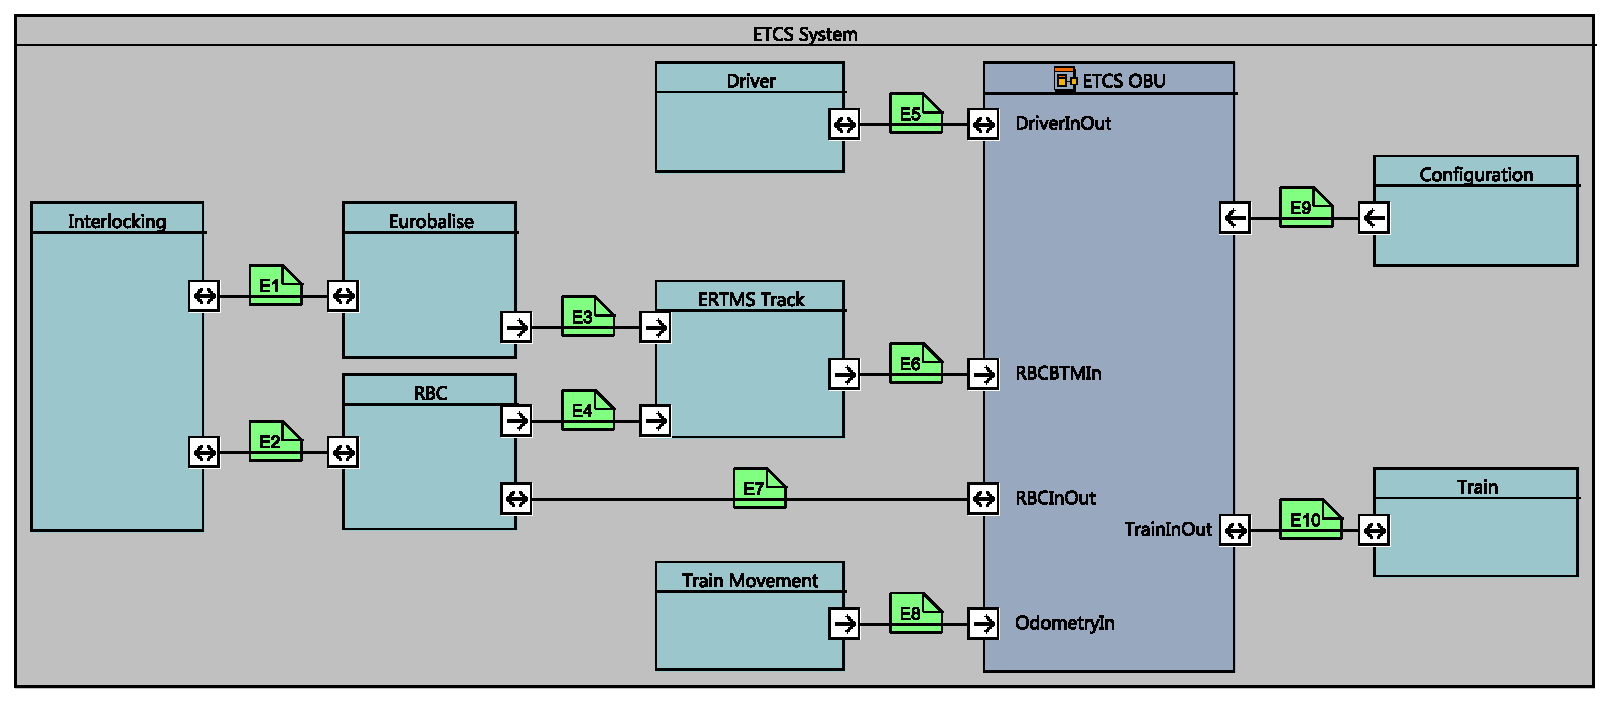
\includegraphics[width=\textwidth]{ETCS_system.pdf}
\caption{Top level architecture with external interfaces E1 to E10.}
\label{f:top_level}
\end{figure}

\todo[inline]{Descriptions should be improved}
\begin{description}
\item[E1:] In- and out flow between the Interlocking and the Eurobalise. Only relevant for controlled Eurobalises.

\item[E2:] Input and output interface between the Interlocking and Radio Block Center (RBC).

\item[E3:] Input interface from the Eurobalise to the ERTMS Track module.

\item[E4:] Input interface from the RBC to the ERTMS Track module.

\item[E5:] This interface is used for the interaction between the driver and the display (Driver Machine Interface, DMI).

\item[E6:] This interface is a compound structure and combines the interfaces E3 and E4 to send track side messages from Eurobalises or RBC to the ETCS OBU.

\item[E7:] Input and output interface between RBC and ETCS OBU. This interface is used for the management of radio communication, e.g.~session management, and sending radio messages from the ETCS OBU to the RBC. Note that the ETCS OBU receives radio messages via interface E6.

\item[E8:] Input interface to the odometry subsystem of the ETCS OBU. Used for sending information to the train if there is any movement outside the ETCS system, e.g.~"cold movement".

\item[E9:] Input interface to the ETCS OBU to set configuration data such as fixed values, system values, national values and train configuration.

\item[E10:] Input and output interface between the ETCS OBU and the train. This interface is used for the interaction between the train and the ETCS OBU such as brake control, traction control, door control, etc.
\end{description}


\section{Functional breakdown of the ETCS OBU}

Figure \ref{f:ETCS_OBU_decomposition} depicts the functional breakdown of the ETCS OBU block shown in Figure~\ref{f:top_level}. The ETCS OBU consits out of 7 functional modules. These are:
\begin{figure}
\centering
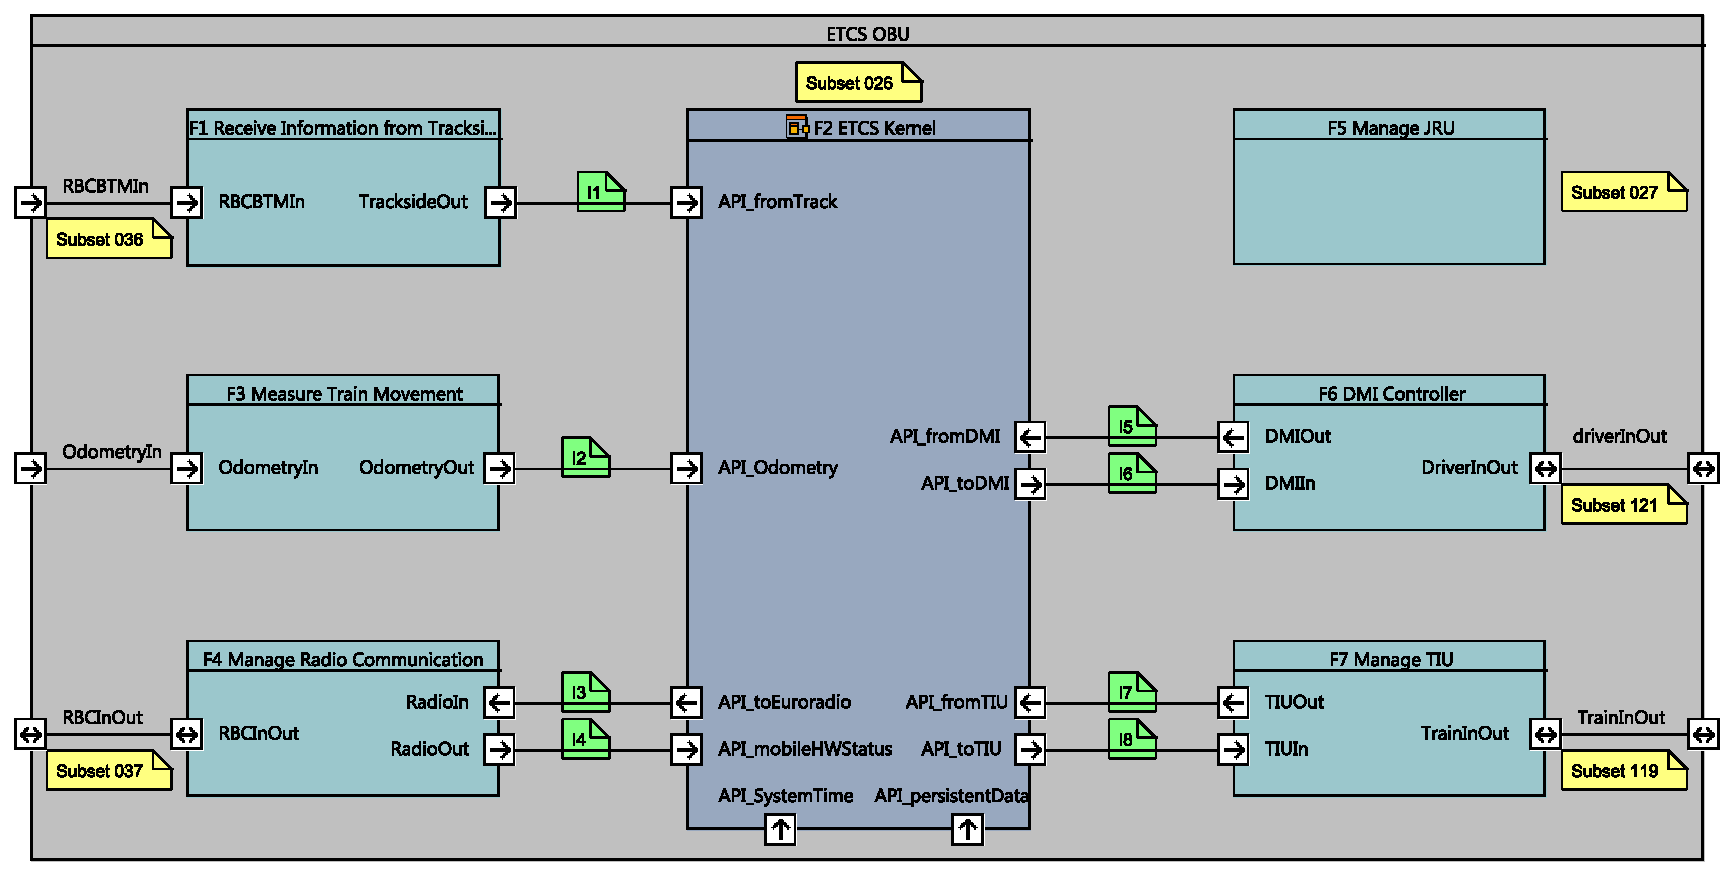
\includegraphics[width=\textwidth]{images/F2_ETCS_Kernel.pdf}
\caption{ETCS OBU system architecture view with internal interfaces I1 to I8.}
\label{f:ETCS_OBU_decomposition}
\end{figure}
\todo[inline]{Component descriptions need to be completed}
\begin{description}
\item[F1 Receive Information from Trackside] This module is responsible for receiving RBC and BTM messages and passing these to the F2 ETCS Kernel module. A detailed description is given in Chapter~\ref{s:F1}.
\item[F2 ETCS Kernel] This module represents core component of the openETCS OBU. A detailed description is given in Chapter~\ref{s:F2}.
\item[F3 Measure Train Movement] This module provides odometry data to the F2 ETCS Kernel module.
\item[F4 Manage Radio Communication]
\item[F5 Manage JRU] This component manages the juridical date. Note that this component is not included in the functional scope of the openETCS OBU respectively project currently.
\item[F6 DMI Controller]
\item[F7 Manage TIU]
\end{description}

These components are interacting via the internal interfaces I1 to I8. In the following we give a brief description of the interfaces.
\begin{description}
\item[I1:] Input interface that allows the F2 ETCS Kernel module to receive information from the Balise Transmission Module as well as the Radio Block Center.

\item[I2:] Input interface from the Odometry (ODO) to the F2 ETCS Kernel module.

\item[I3:] Output interface between the F4 Manage Radio Communication module and the F2 ETCS Kernel module. This interface is used for radio session management and sending radio messages from the OBU to the track side.

\item[I4:] Input interface between the F4 Manage Radio Communication module and the F2 ETCS Kernel module.

\item[I5:] Input interface between the F6 DMI Controller module and the F2 ETCS Kernel module.

\item[I6:] Output interface between the F6 DMI Controller module and the F2 ETCS Kernel module.

\item[I7:] Input interface between the F7 Manage TIU module and the F2 ETCS Kernel module.

\item[I8:] Output interface between the F7 Manage TIU module and the F2 ETCS Kernel module.
\end{description}









%\chapter{Software Architecture}
%t.b.d.\todo[fancyline]{has to be completed}



\part{Design Description}

\chapter{General Design Decisions}

\input{sections/general_design_decisions.tex}


\chapter{F1: Receive Information from Trackside}\label{s:F1}

\input{sections/trackside.tex}


\chapter{F2: ETCS Kernel}\label{s:F2}

In this chapter we describe the main components of the openETCS OBU model. Section~\ref{s:ETCS_Kernel_Overview} gives an overview of the external interfaces of this functional block and gives a brief overview of its components and their interaction. The following Sections~\ref{s:F2.1} to \ref{s:F2.13} give a detailed description for each of the components in F2: ETCS Kernel.

\section{ETCS Kernel Overview}\label{s:ETCS_Kernel_Overview}

The ETCS Kernel module consists of the 13 functional components, i.e. F2.1 to F2.13 as depicted in Figures~\ref{f:f2.1_overview} to \ref{f:f2.13_overview}. Note that due to the complexity of the Kernel module the SysML diagram has been splitted into 13 figures. Each of the figures shows one of the subcomponents F2.1 to F2.13 and its connections to the other components in F2 and the inputs respectively outputs of F2. In the following we briefly describe the functionality of these components.
\begin{description}
\item[F2.1: Manage\_TrackSideInformation\_Integration] This component is responsible for receiving Eurobalise telegrams and Euroradio messages from the API and performs several consistency checks on the inputs. The corresponding SysML diagram is shown in Figure~\ref{f:f2.1_overview}. For further details we refer to Section~\ref{s:F2.1}.

\item[F2.2: Manage\_ETCS\_Procedures] This component describes the Start of Mission procedure of the train until the current status will change to another mode, level or other procedure. The corresponding SysML diagram is shown in Figure~\ref{f:f2.2_overview}. For further details we refer to Section~\ref{s:F2.2}.

\item[F2.3: trainData] Implementation of the train data with the corresponding interfaces to track, driver and RBC. The corresponding SysML diagram is shown in Figure~\ref{f:f2.3_overview}. For further details we refer to Section~\ref{s:F2.3}.
\todo[inline]{descriptions needs to be improved}

\item[F2.4: TrackAtlas] t.b.d.  The corresponding SysML diagram is shown in Figure~\ref{f:f2.4_overview}. For further details we refer to Section~\ref{s:F2.4}.
\todo[inline]{to be completed}

\item[F2.5: ManageLevelAndMode] Defines the status of the ETCS regarding on-board functional status and track infrastructure. The corresponding SysML diagram is shown in Figure~\ref{f:f2.5_overview}. For further details we refer to Section~\ref{s:F2.5}.
\todo[inline]{descriptions needs to be improved}

\item[F2.6: calculateTrainPosition] The purpose of this component is to calculate the locations of linked and unlinked balise groups and the current train position while the train is running along the track. The corresponding SysML diagram is shown in Figure~\ref{f:f2.6_overview}. For further details we refer to Section~\ref{s:F2.6}.


\item[F2.7: SpeedSupervision\_Integration] This component monitors the current speed of the train and its location to ensure that the speed remains within the given speed and distance limits. The corresponding SysML diagram is shown in Figure~\ref{f:f2.7_overview}. For further details we refer to Section~\ref{s:F2.7}.


\item[F2.8: Provide\_Position\_Report] The component builds a position report for the RBC, i.e., message 132, and provides it as an output. The corresponding SysML diagram is shown in Figure~\ref{f:f2.8_overview}. For further details we refer to Section~\ref{s:F2.8}.


\item[F2.9: Manage\_Radio\_Communication] This component implements the onboard management of a single communication session with the track, i.e.~a single RBC. It controls the establishment, maintenance and termination process of a radio communication session and steers the underlying communication safety layer as well as the mobile device. Those and the data transfer itself are not part of this component. The corresponding SysML diagram is shown in Figure~\ref{f:f2.9_overview}. For further details we refer to Section~\ref{s:F2.9}.


\item[F2.10: manageDMI\_input] This component handles messages respectively data coming from the Driver Machine Interface (DMI) to the ETCS OBU. The corresponding SysML diagram is shown in Figure~\ref{f:f2.10_overview}. For further details we refer to Section~\ref{s:F2.10}.


\item[F2.11: manageDMI\_output] This component handles messages respectively data being send from the ETCS OBU to the DMI. The corresponding SysML diagram is shown in Figure~\ref{f:f2.11_overview}. For further details we refer to Section~\ref{s:F2.11}.


\item[F2.12: manageTIU\_input] This component handles messages respectively data coming from the Train Interface Unit (TIU) to the ETCS OBU. The corresponding SysML diagram is shown in Figure~\ref{f:f2.12_overview}. For further details we refer to Section~\ref{s:F2.12}.


\item[F2.13: manageTIU\_output] This component handles messages respectively data being send from the ETCS OBU to the TIU. The corresponding SysML diagram is shown in Figure~\ref{f:f2.13_overview}. For further details we refer to Section~\ref{s:F2.13}.
\end{description}

\begin{figure}
\center
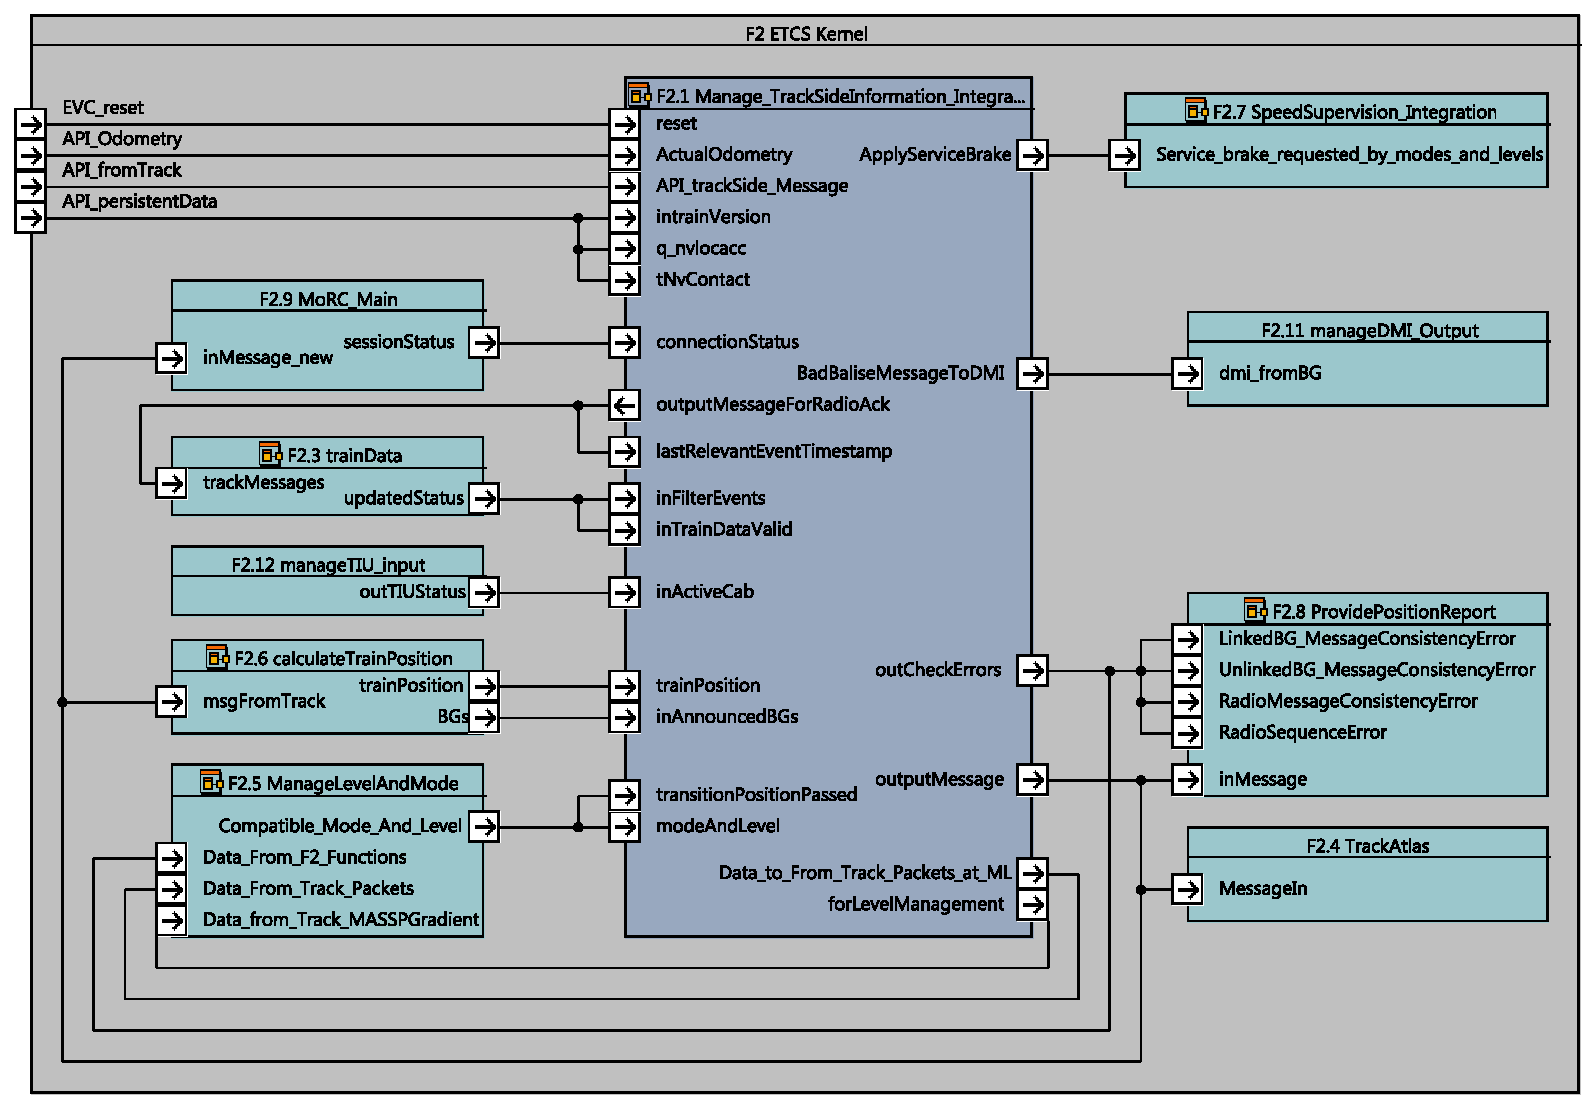
\includegraphics[width=\textwidth]{F2_F2_1.pdf}
\caption{F2: ETCS Kernel SysML diagram with focus on F2.1 Manage\_TrackSideInformation\_Integration component.}\label{f:f2.1_overview}
\end{figure}

\begin{figure}
\center
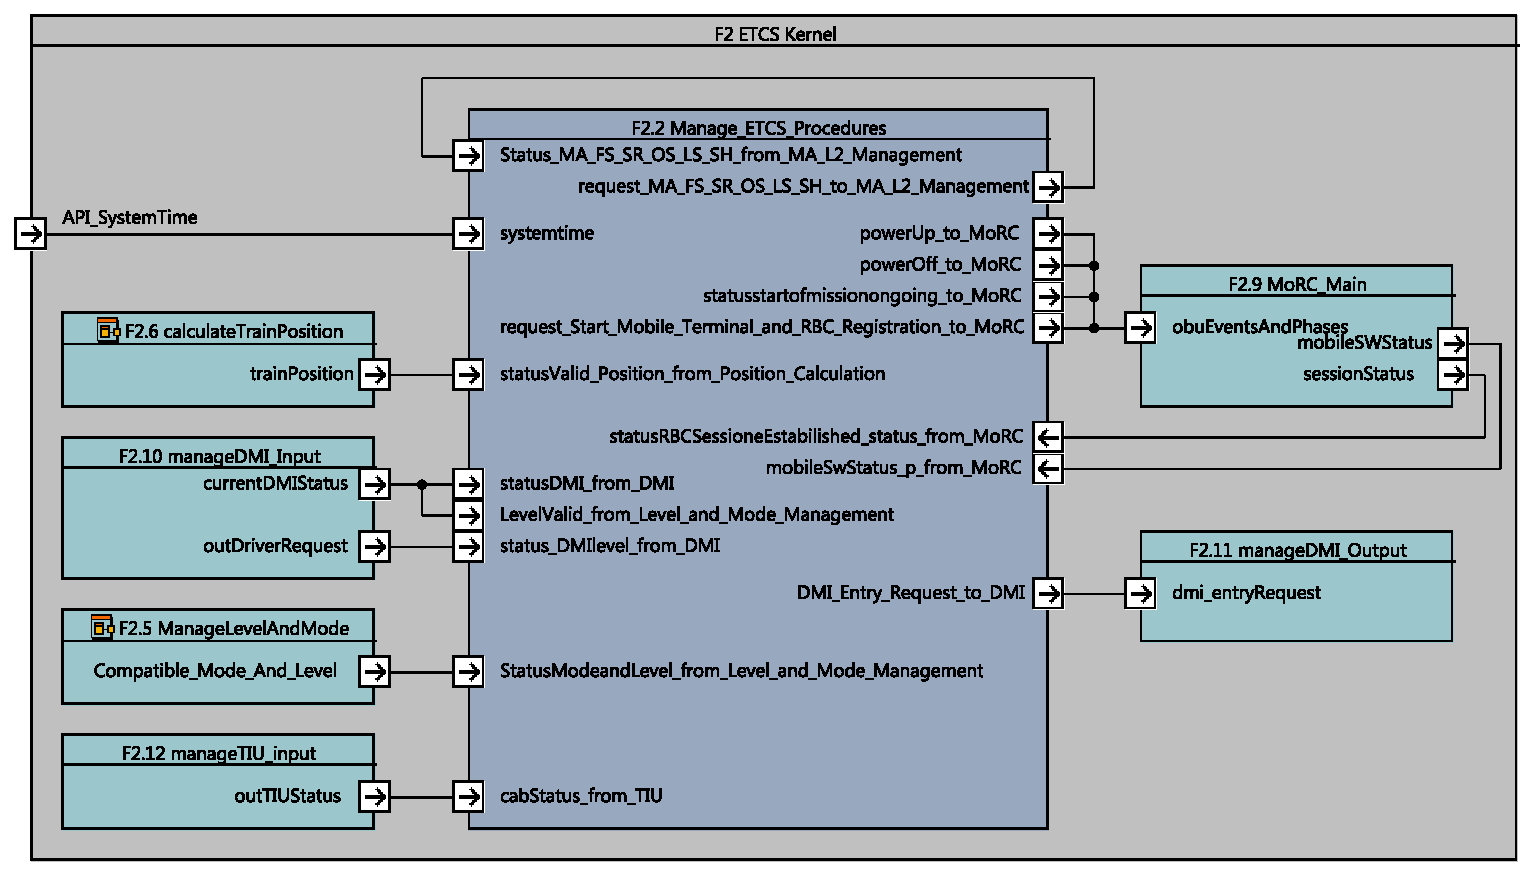
\includegraphics[width=\textwidth]{F2_F2_2.pdf}
\caption{F2: ETCS Kernel SysML diagram with focus on F2.2 Manage\_ETCS\_Procedures component.}\label{f:f2.2_overview}
\end{figure}

\begin{figure}
\center
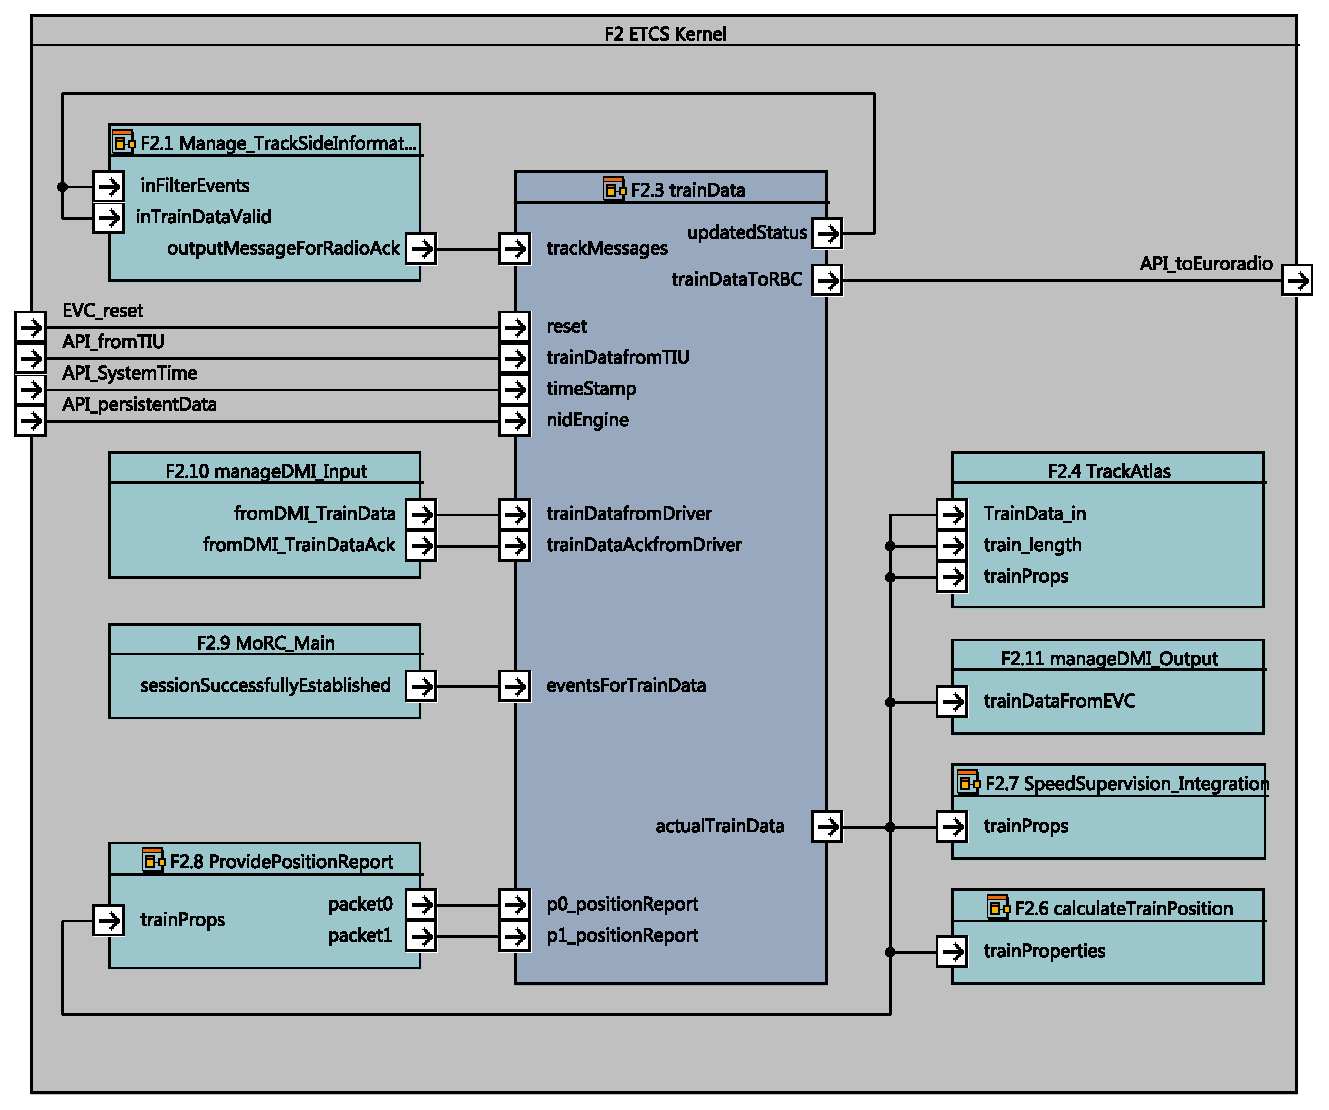
\includegraphics[width=\textwidth]{F2_F2_3.pdf}
\caption{F2: ETCS Kernel SysML diagram with focus on F2.3 trainData component.}\label{f:f2.3_overview}
\end{figure}

\begin{figure}
\center
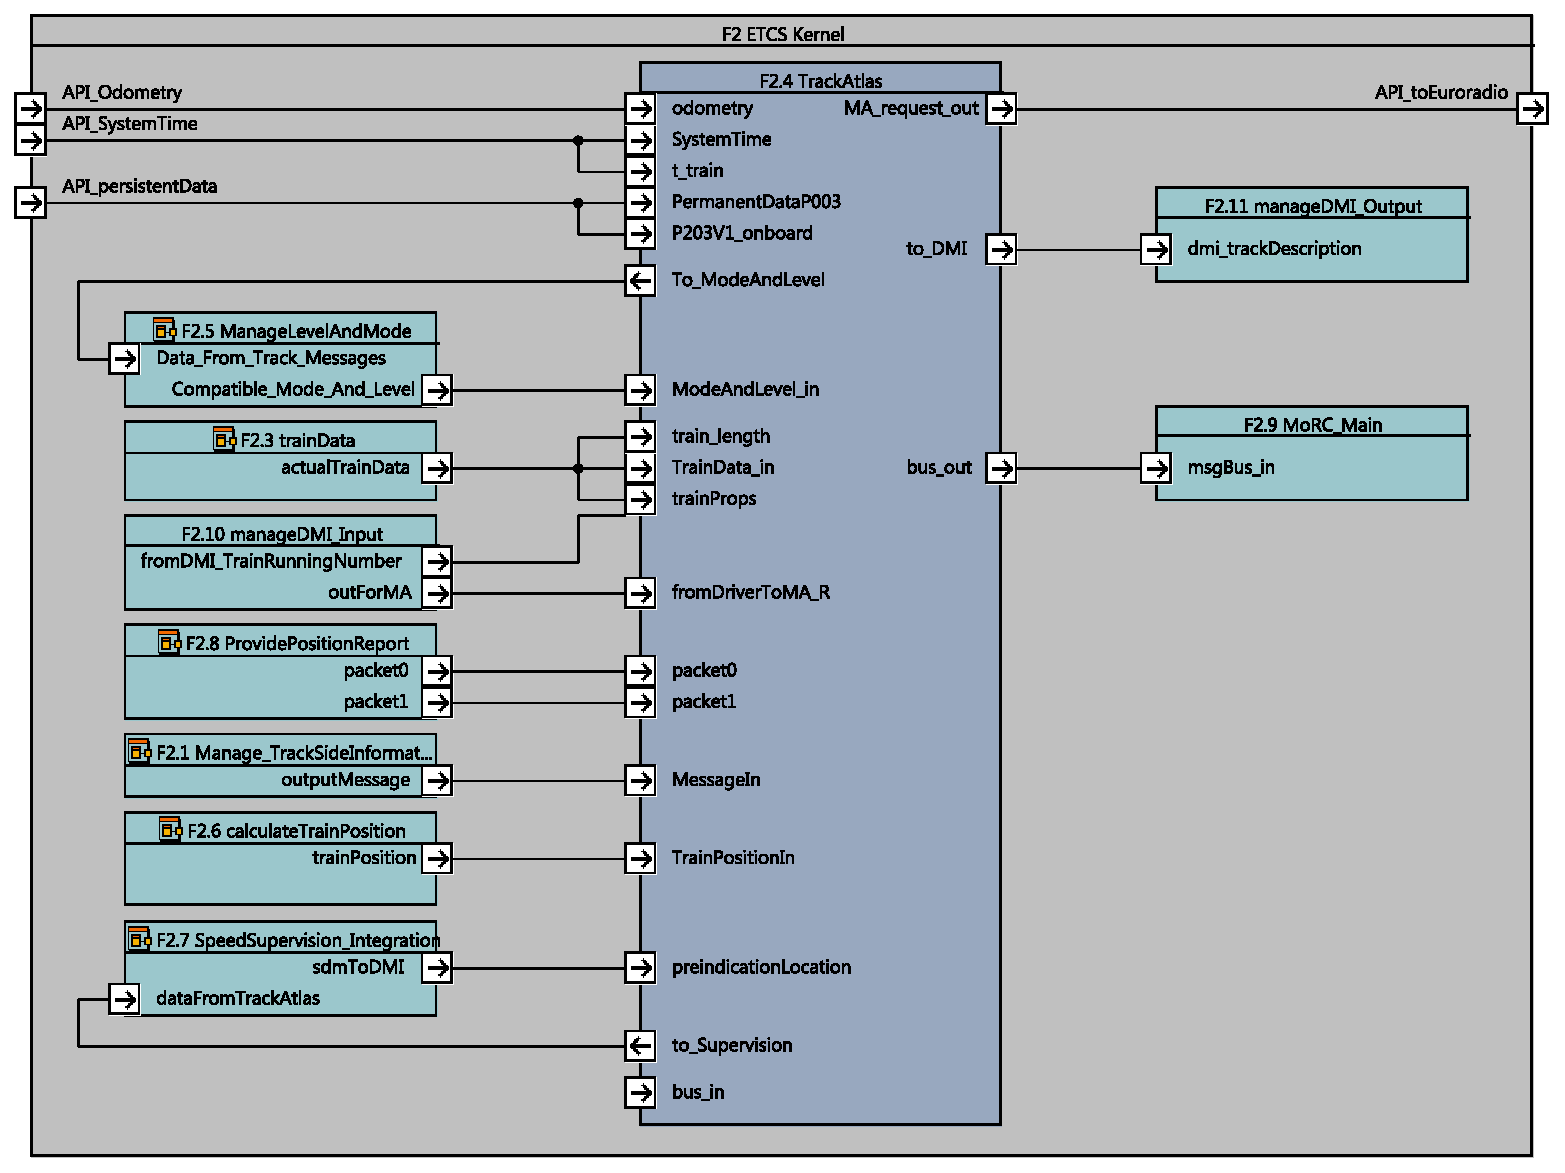
\includegraphics[width=\textwidth]{F2_F2_4.pdf}
\caption{F2: ETCS Kernel SysML diagram with focus on F2.4 TrackAtlas component.}\label{f:f2.4_overview}
\end{figure}

\begin{figure}
\center
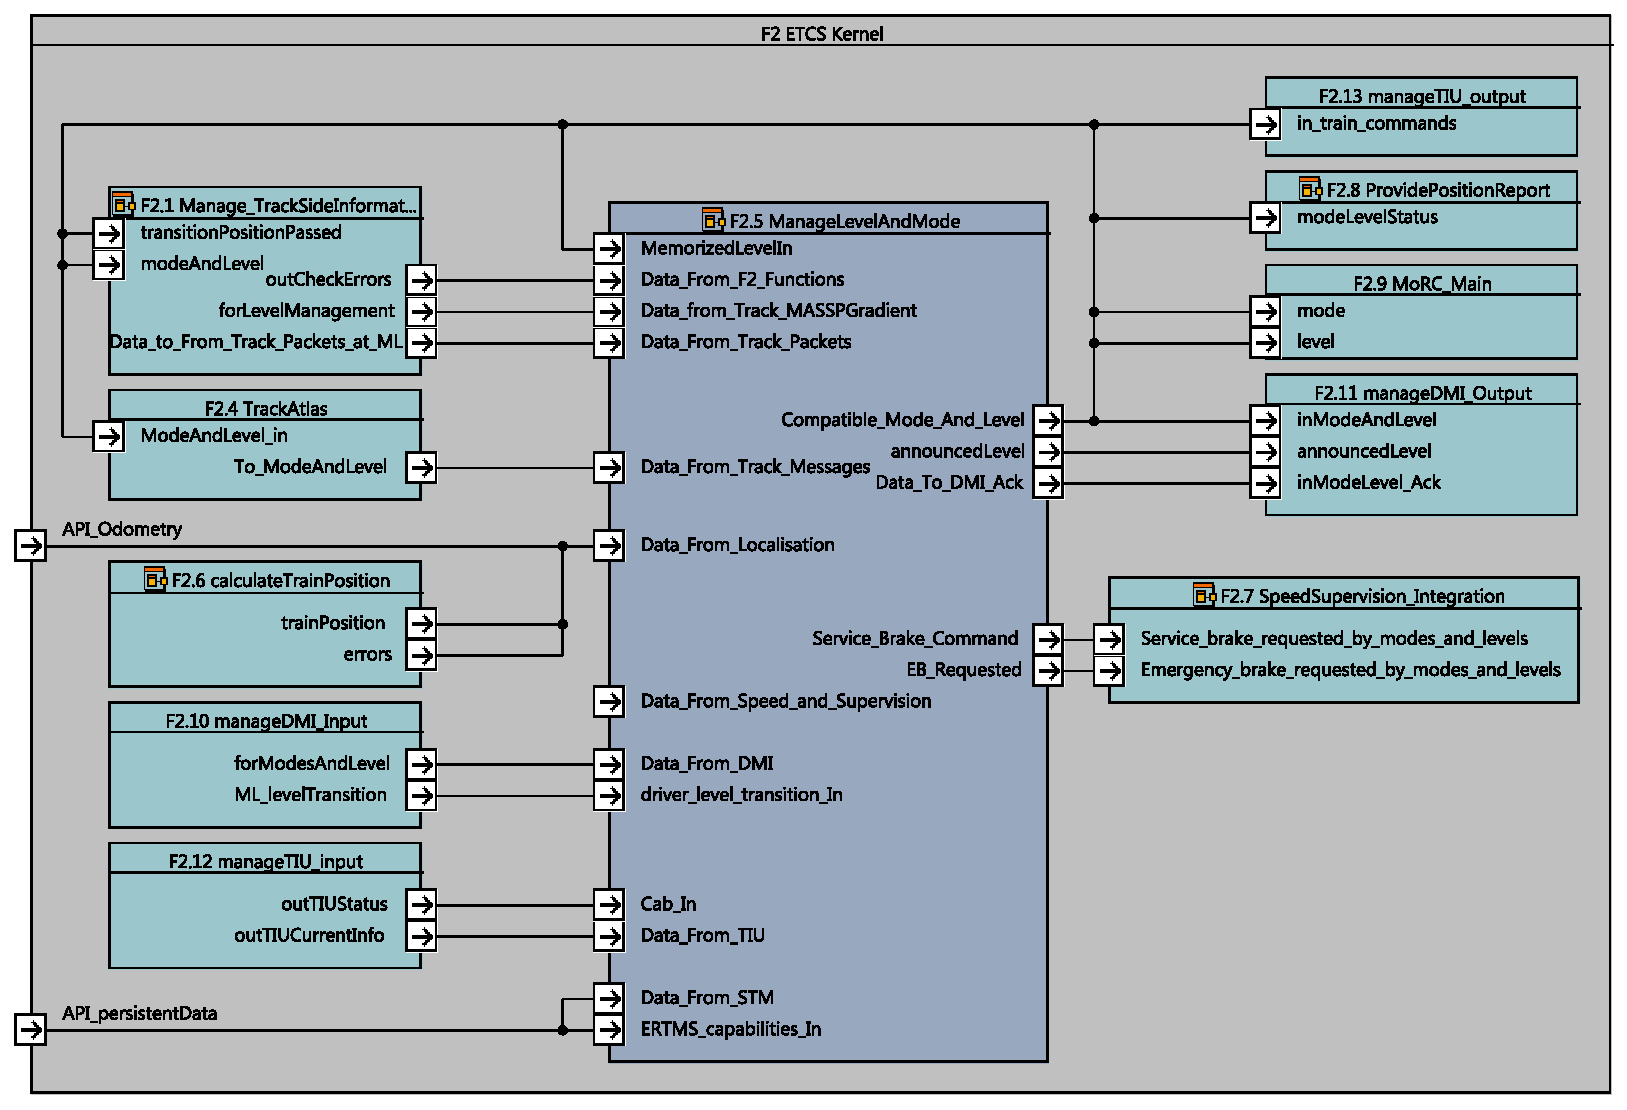
\includegraphics[width=\textwidth]{F2_F2_5.pdf}
\caption{F2: ETCS Kernel SysML diagram with focus on F2.5 Mode\_and\_Level component.}\label{f:f2.5_overview}
\end{figure}

\begin{figure}
\center
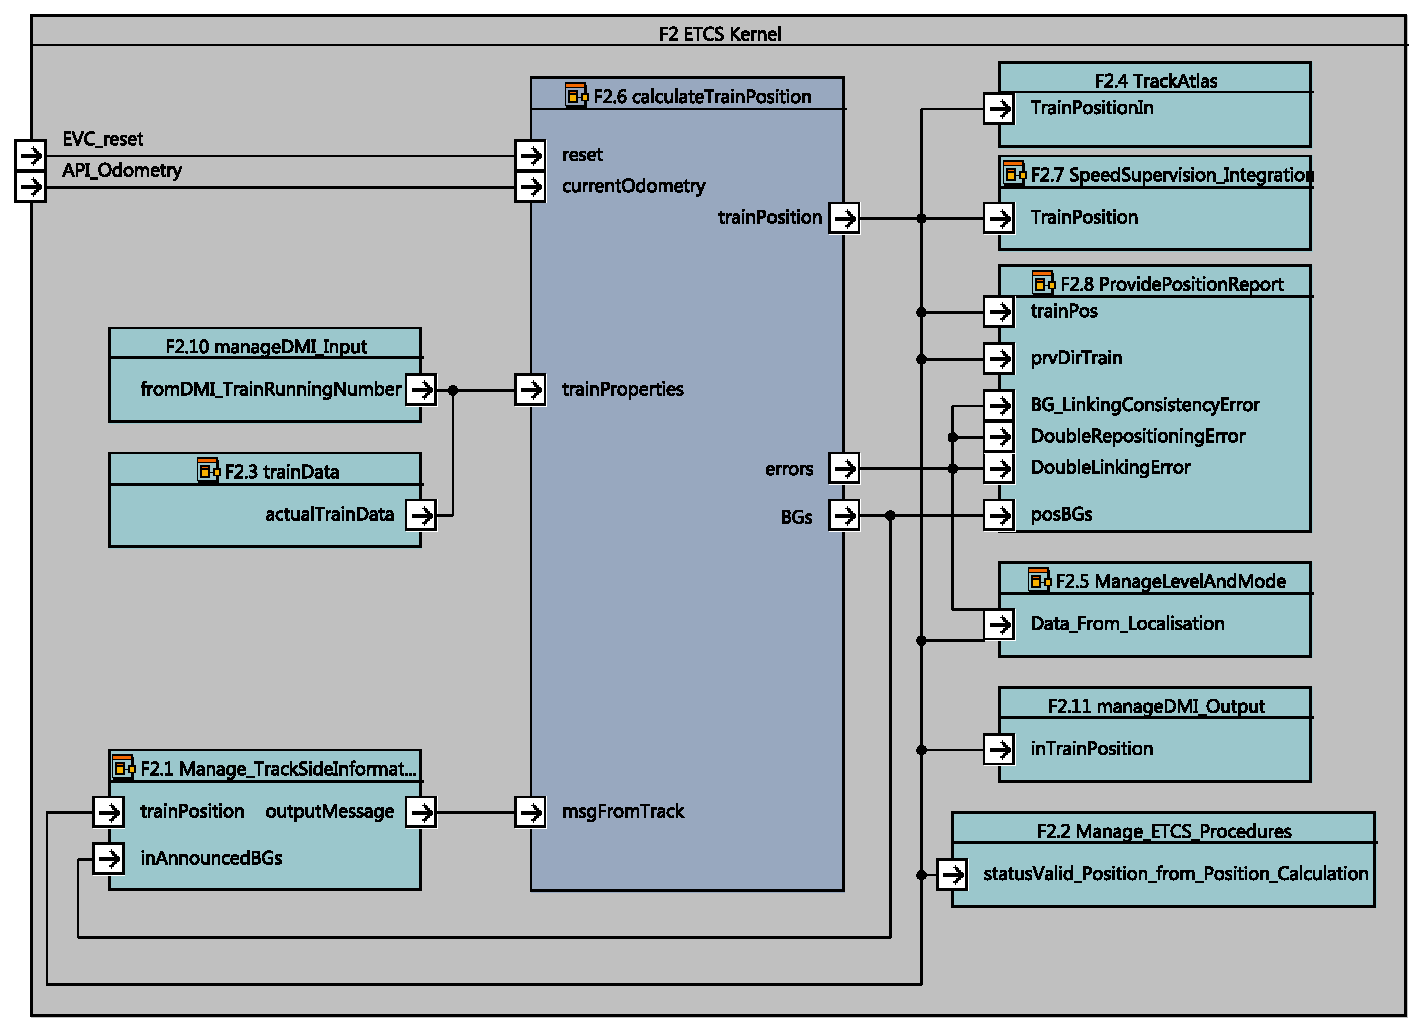
\includegraphics[width=\textwidth]{F2_F2_6.pdf}
\caption{F2: ETCS Kernel SysML diagram with focus on F2.6 calculateTrainPosition component.}\label{f:f2.6_overview}
\end{figure}

\begin{figure}
\center
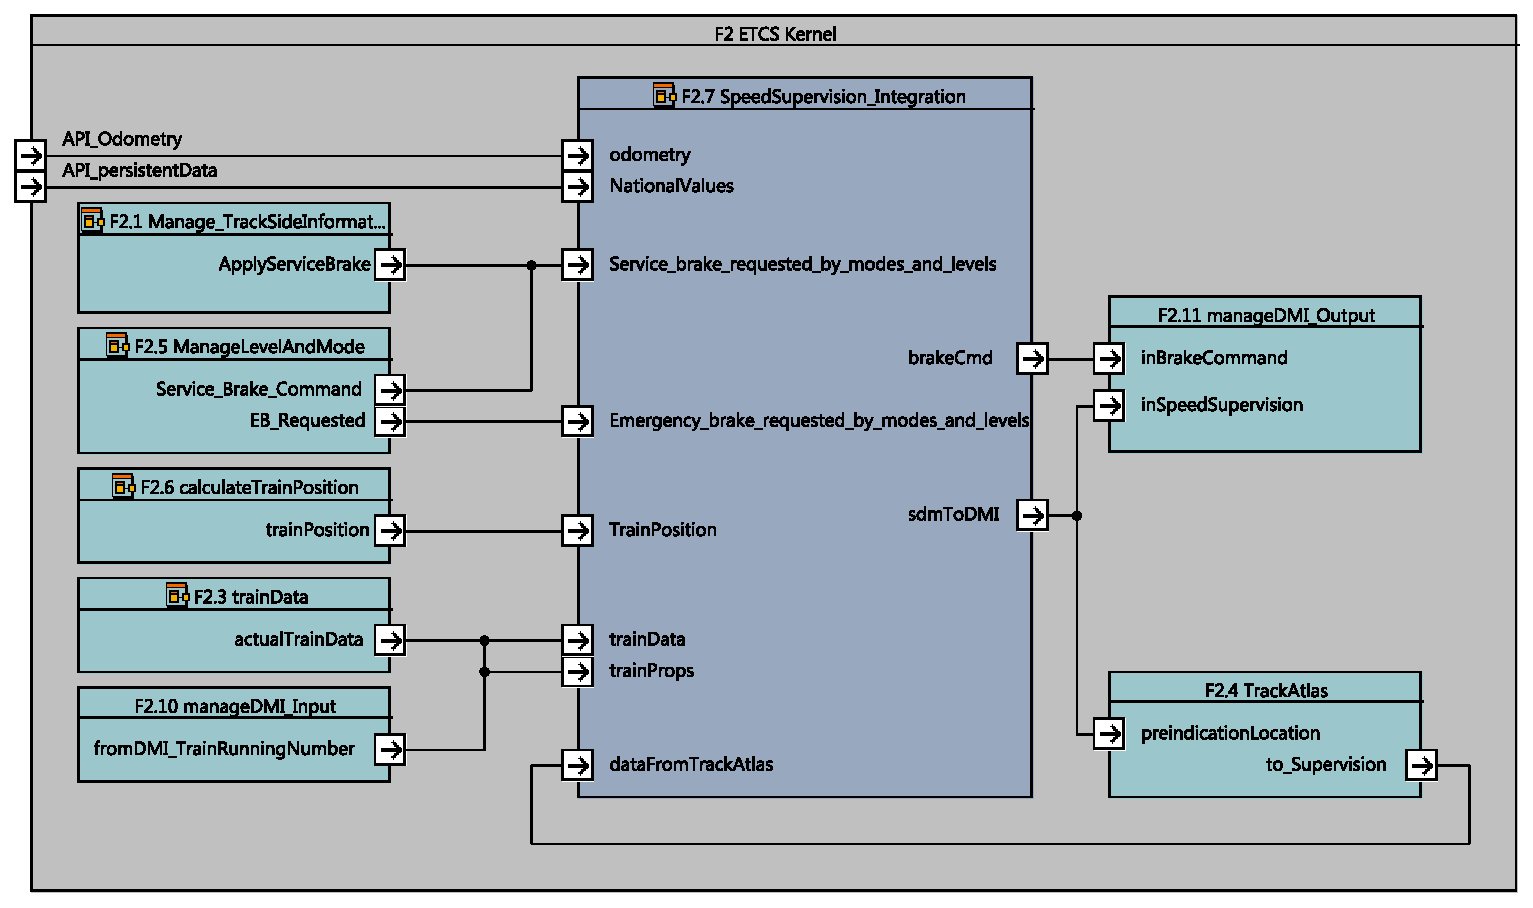
\includegraphics[width=\textwidth]{F2_F2_7.pdf}
\caption{F2: ETCS Kernel SysML diagram with focus on F2.7 SpeedSupervision\_Integration component.}\label{f:f2.7_overview}
\end{figure}

\begin{figure}
\center
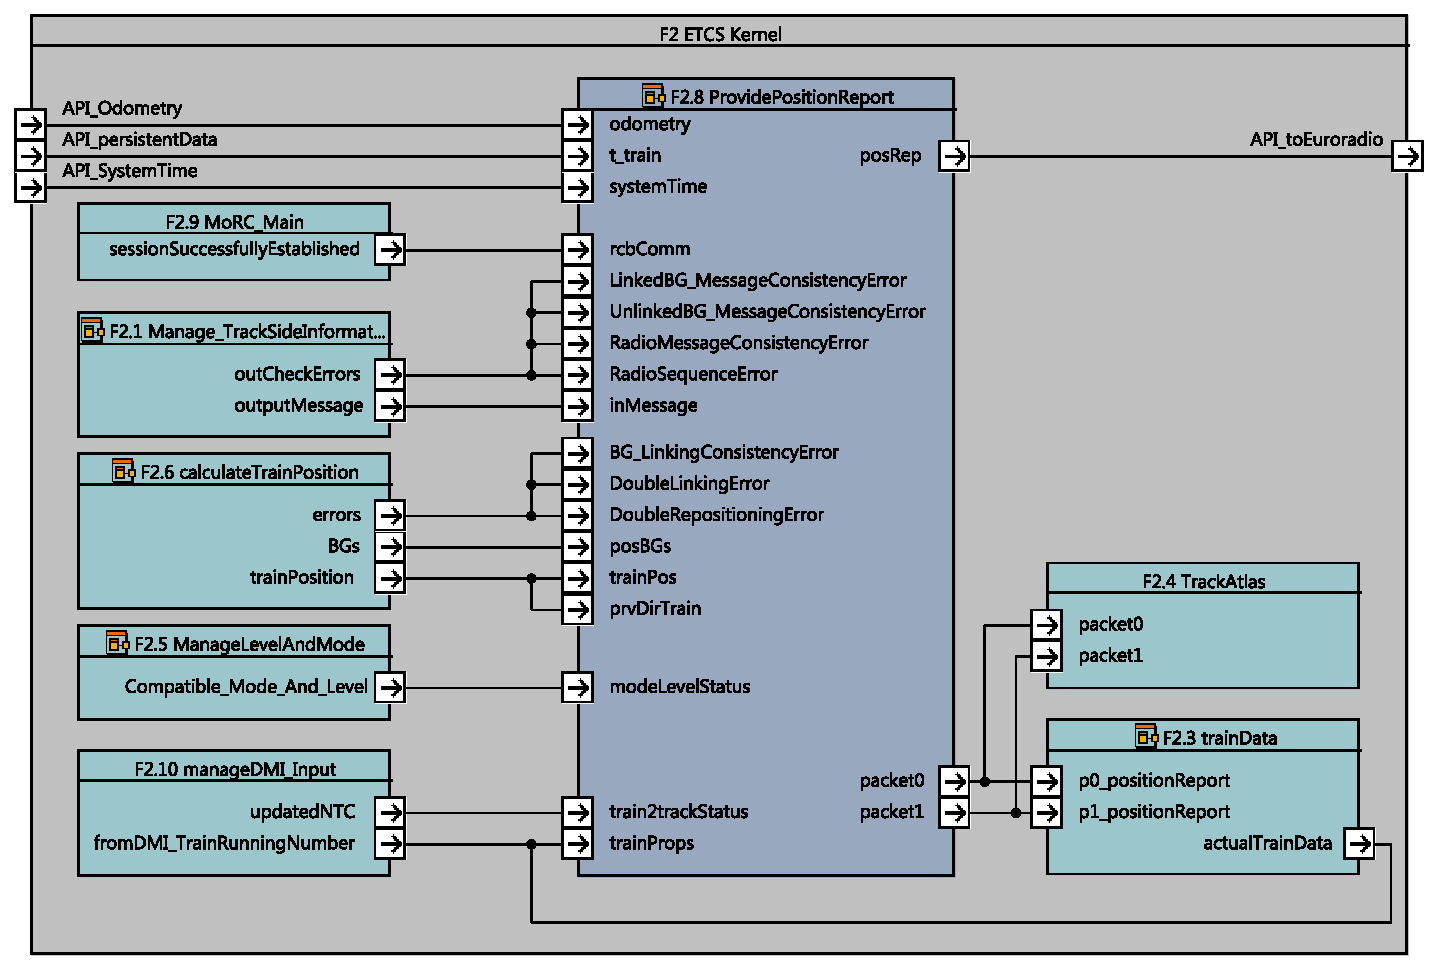
\includegraphics[width=\textwidth]{F2_F2_8.pdf}
\caption{F2: ETCS Kernel SysML diagram with focus on F2.8 Provide\_Position\_Report component.}\label{f:f2.8_overview}
\end{figure}

\begin{figure}
\center
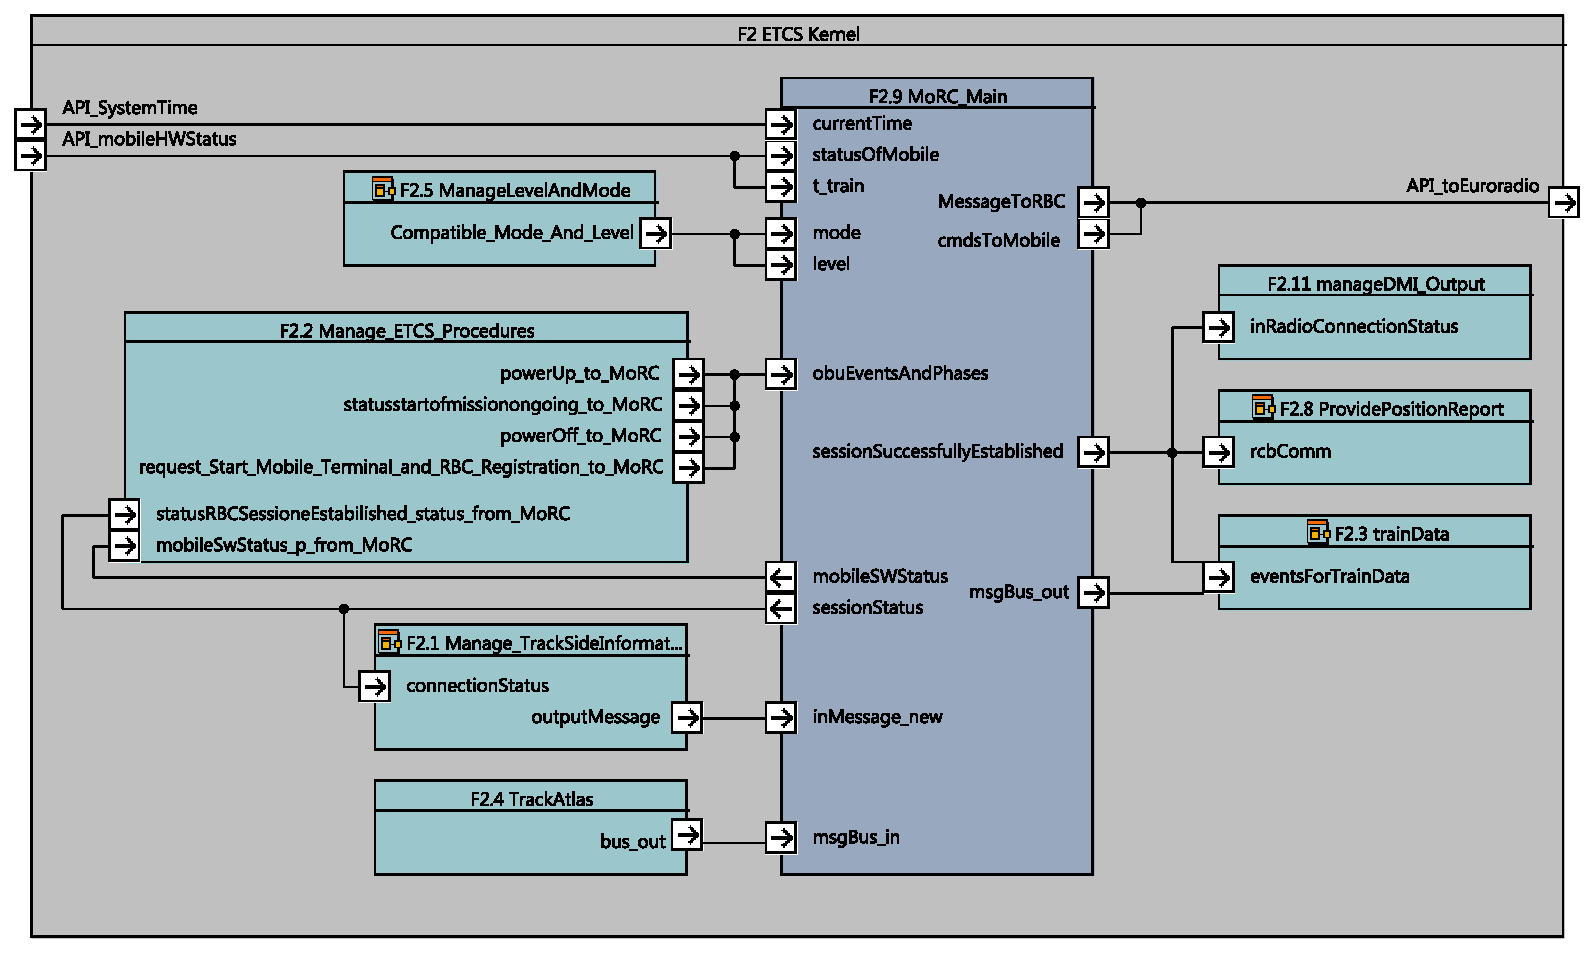
\includegraphics[width=\textwidth]{F2_F2_9.pdf}
\caption{F2: ETCS Kernel SysML diagram with focus on F2.9 Manage\_Radio\_Communication component.}\label{f:f2.9_overview}
\end{figure}

\begin{figure}
\center
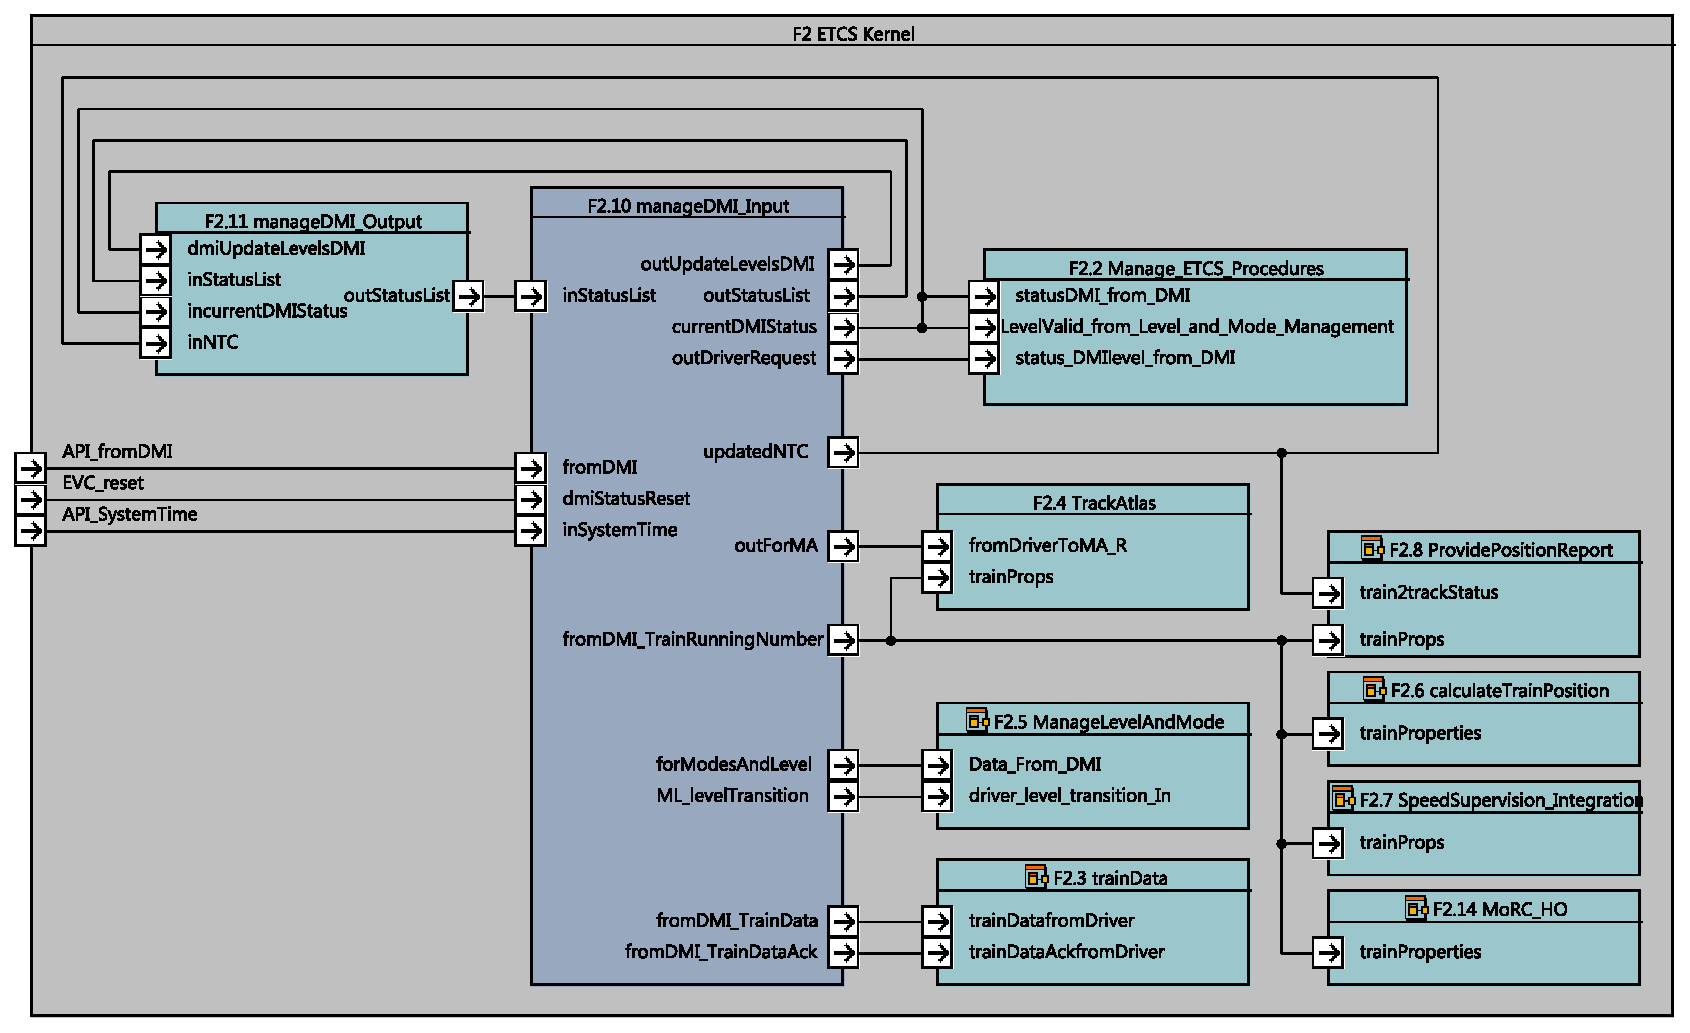
\includegraphics[width=\textwidth]{F2_F2_10.pdf}
\caption{F2: ETCS Kernel SysML diagram with focus on F2.10 ManageDMIInput component.}\label{f:f2.10_overview}
\end{figure}

\begin{figure}
\center
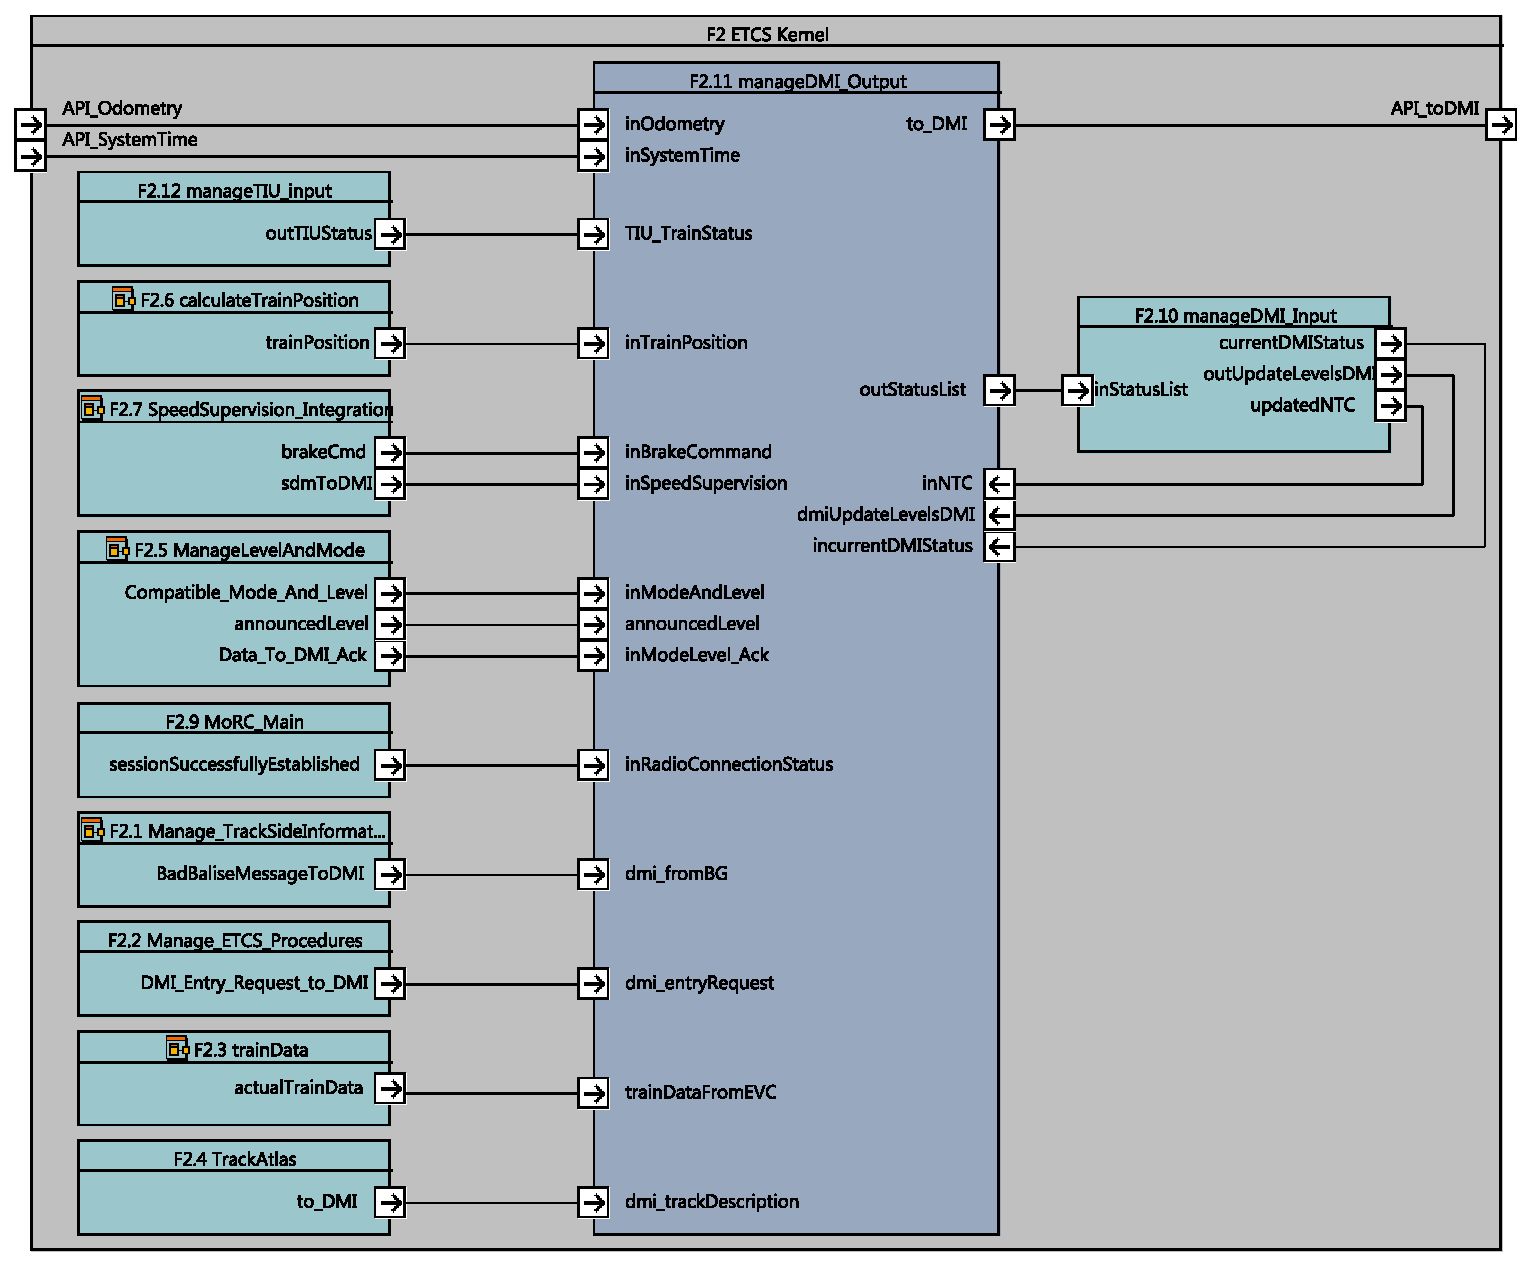
\includegraphics[width=\textwidth]{F2_F2_11.pdf}
\caption{F2: ETCS Kernel SysML diagram with focus on F2.11 ManageDMIOutput component.}\label{f:f2.11_overview}
\end{figure}

\begin{figure}
\center
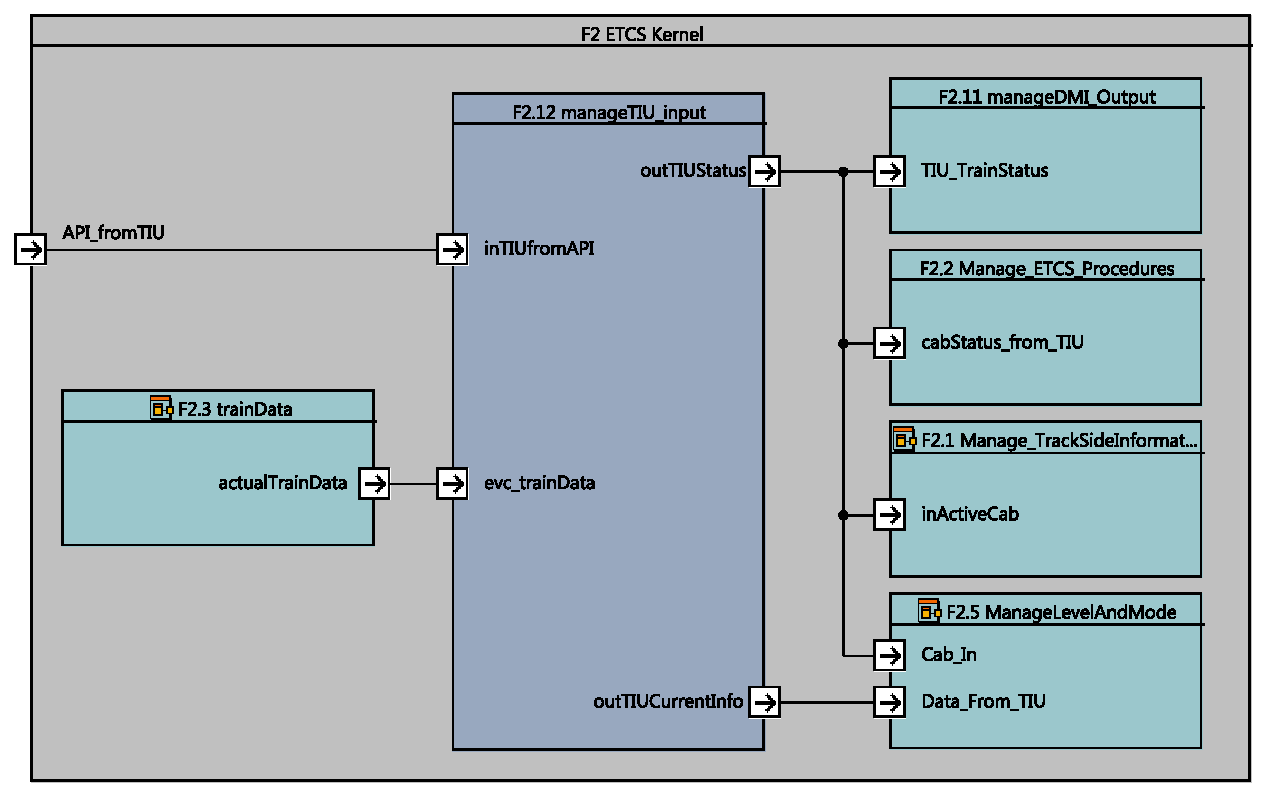
\includegraphics[width=\textwidth]{F2_F2_12.pdf}
\caption{F2: ETCS Kernel SysML diagram with focus on F2.12 ManageTIUInput component.}\label{f:f2.12_overview}
\end{figure}

\begin{figure}
\center
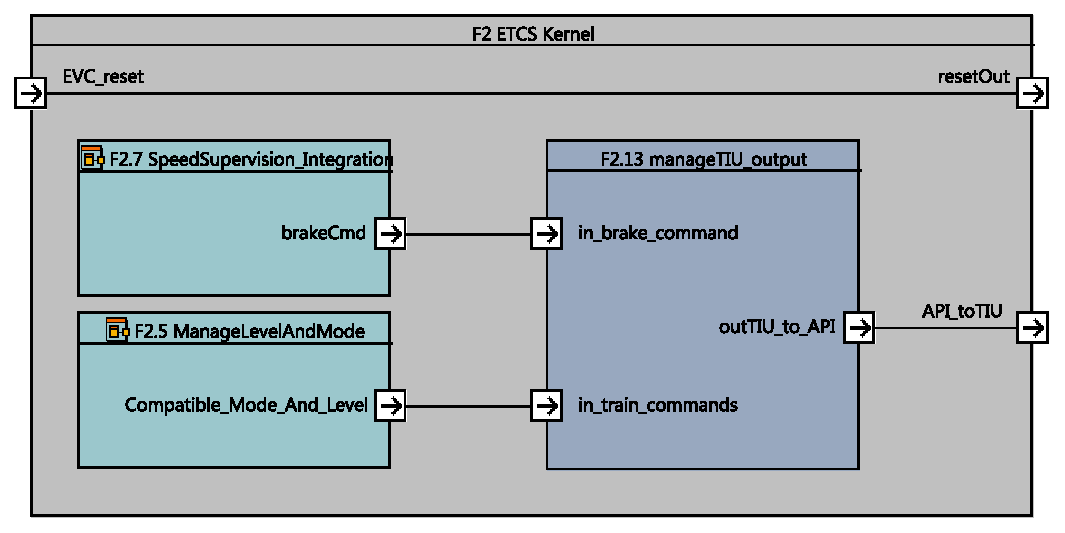
\includegraphics[width=\textwidth]{F2_F2_13.pdf}
\caption{F2: ETCS Kernel SysML diagram with focus on F2.13 ManageTIUOutput component.}\label{f:f2.13_overview}
\end{figure}
















\subsection{External Interfaces}
This section gives a detailed overview of the external inputs and outputs of module F2: ETCS Kernel.

\subsubsection{External Inputs}

\paragraph{EVC\_reset}

\begin{longtable}{p{.25\textwidth}p{.7\textwidth}}
\toprule
Input name				& EVC\_reset \\
\midrule
Description				&  The reset input is used to delete all data stored in the connected components inside F2 (e.g.~collected balise telegrams). If the input is set to true, all data kept in the components is deleted and no input is accepted. The reset option is to be used when the EVC is started or in system error scenarios. \\
\midrule
Source					& [Name of the source component] \\ 
\midrule
Type					& [Type of the input] \\
\midrule
Valid range of values	& [Complete list of valid values] \\
\midrule
Behaviour when value is at boundary	& [Description of components behaviour when input value is at boundary] \\
\midrule
Behaviour for values out of valid range	& [Description of components behaviour when input value is out of valid range] \\
\midrule
Behaviour when value is erroneous, absent or unwanted (i.e. spurious) & [Description of components behaviour when value is erroneous, absent or unwanted (i.e. spurious)] \\
\bottomrule
\end{longtable}

\paragraph{API\_Odometry}

\begin{longtable}{p{.25\textwidth}p{.7\textwidth}}
\toprule
Input name				& API\_Odometry \\
\midrule
Description				& Odometry data provided by the external odometry module of the train. \\
\midrule
Source					& API \\ 
\midrule
Type					& [Type of the input] \\
\midrule
Valid range of values	& [Complete list of valid values] \\
\midrule
Behaviour when value is at boundary	& [Description of components behaviour when input value is at boundary] \\
\midrule
Behaviour for values out of valid range	& [Description of components behaviour when input value is out of valid range] \\
\midrule
Behaviour when value is erroneous, absent or unwanted (i.e. spurious) & [Description of components behaviour when value is erroneous, absent or unwanted (i.e. spurious)] \\
\bottomrule
\end{longtable}

\paragraph{API\_SystemTime}

\begin{longtable}{p{.25\textwidth}p{.7\textwidth}}
\toprule
Input name				& API\_SystemTime \\
\midrule
Description				& [Brief description of the input] \\
\midrule
Source					& API \\ 
\midrule
Type					& [Type of the input] \\
\midrule
Valid range of values	& [Complete list of valid values] \\
\midrule
Behaviour when value is at boundary	& [Description of components behaviour when input value is at boundary] \\
\midrule
Behaviour for values out of valid range	& [Description of components behaviour when input value is out of valid range] \\
\midrule
Behaviour when value is erroneous, absent or unwanted (i.e. spurious) & [Description of components behaviour when value is erroneous, absent or unwanted (i.e. spurious)] \\
\bottomrule
\end{longtable}

\paragraph{API\_fromTrack}

\begin{longtable}{p{.25\textwidth}p{.7\textwidth}}
\toprule
Input name				& API\_fromTrack \\
\midrule
Description				& [Brief description of the input] \\
\midrule
Source					& API respectively F1 Receive Information from Trackside\\ 
\midrule
Type					& [Type of the input] \\
\midrule
Valid range of values	& [Complete list of valid values] \\
\midrule
Behaviour when value is at boundary	& [Description of components behaviour when input value is at boundary] \\
\midrule
Behaviour for values out of valid range	& [Description of components behaviour when input value is out of valid range] \\
\midrule
Behaviour when value is erroneous, absent or unwanted (i.e. spurious) & [Description of components behaviour when value is erroneous, absent or unwanted (i.e. spurious)] \\
\bottomrule
\end{longtable}

\paragraph{API\_fromDMI}

\begin{longtable}{p{.25\textwidth}p{.7\textwidth}}
\toprule
Input name				& API\_fromDMI \\
\midrule
Description				& [Brief description of the input] \\
\midrule
Source					& API respectively F6 DMI Controller\\ 
\midrule
Type					& [Type of the input] \\
\midrule
Valid range of values	& [Complete list of valid values] \\
\midrule
Behaviour when value is at boundary	& [Description of components behaviour when input value is at boundary] \\
\midrule
Behaviour for values out of valid range	& [Description of components behaviour when input value is out of valid range] \\
\midrule
Behaviour when value is erroneous, absent or unwanted (i.e. spurious) & [Description of components behaviour when value is erroneous, absent or unwanted (i.e. spurious)] \\
\bottomrule
\end{longtable}

\paragraph{API\_fromTIU}

\begin{longtable}{p{.25\textwidth}p{.7\textwidth}}
\toprule
Input name				& API\_fromTIU \\
\midrule
Description				& [Brief description of the input] \\
\midrule
Source					& API respectively F7 Manage TIU Interface \\ 
\midrule
Type					& [Type of the input] \\
\midrule
Valid range of values	& [Complete list of valid values] \\
\midrule
Behaviour when value is at boundary	& [Description of components behaviour when input value is at boundary] \\
\midrule
Behaviour for values out of valid range	& [Description of components behaviour when input value is out of valid range] \\
\midrule
Behaviour when value is erroneous, absent or unwanted (i.e. spurious) & [Description of components behaviour when value is erroneous, absent or unwanted (i.e. spurious)] \\
\bottomrule
\end{longtable}

\paragraph{API\_mobileHWStatus}

\begin{longtable}{p{.25\textwidth}p{.7\textwidth}}
\toprule
Input name				& API\_mobileHWStatus \\
\midrule
Description				& [Brief description of the input] \\
\midrule
Source					& [Name of the source component] \\ 
\midrule
Type					& [Type of the input] \\
\midrule
Valid range of values	& [Complete list of valid values] \\
\midrule
Behaviour when value is at boundary	& [Description of components behaviour when input value is at boundary] \\
\midrule
Behaviour for values out of valid range	& [Description of components behaviour when input value is out of valid range] \\
\midrule
Behaviour when value is erroneous, absent or unwanted (i.e. spurious) & [Description of components behaviour when value is erroneous, absent or unwanted (i.e. spurious)] \\
\bottomrule
\end{longtable}

\paragraph{API\_persistentData}

\begin{longtable}{p{.25\textwidth}p{.7\textwidth}}
\toprule
Input name				& API\_persistentData \\
\midrule
Description				& [Brief description of the input] \\
\midrule
Source					& [Name of the source component] \\ 
\midrule
Type					& [Type of the input] \\
\midrule
Valid range of values	& [Complete list of valid values] \\
\midrule
Behaviour when value is at boundary	& [Description of components behaviour when input value is at boundary] \\
\midrule
Behaviour for values out of valid range	& [Description of components behaviour when input value is out of valid range] \\
\midrule
Behaviour when value is erroneous, absent or unwanted (i.e. spurious) & [Description of components behaviour when value is erroneous, absent or unwanted (i.e. spurious)] \\
\bottomrule
\end{longtable}



\subsubsection{External Outputs}

\paragraph{resetOut}

\begin{longtable}{p{.25\textwidth}p{.7\textwidth}}
\toprule
Output name				& resetOut \\
\midrule
Description				& [Brief description of the output] \\
\midrule
Destination				& [Name of the destination component(s)] \\ 
\midrule
Type					& [Type of the output] \\
\midrule
Valid range of values	& [Complete list of valid values] \\
\midrule
Behaviour when value is at boundary	& [Description of components behaviour when output value is at boundary] \\
\midrule
Behaviour for values out of valid range	& [Description of components behaviour when output value is out of valid range] \\
\midrule
Behaviour when value is erroneous, absent or unwanted (i.e. spurious) & [Description of components behaviour when value is erroneous, absent or unwanted (i.e. spurious)] \\
\bottomrule
\end{longtable}


\paragraph{API\_toEuroradio}

\begin{longtable}{p{.25\textwidth}p{.7\textwidth}}
\toprule
Output name				& API\_toEuroradio \\
\midrule
Description				& [Brief description of the output] \\
\midrule
Destination				& [Name of the destination component(s)] \\ 
\midrule
Type					& [Type of the output] \\
\midrule
Valid range of values	& [Complete list of valid values] \\
\midrule
Behaviour when value is at boundary	& [Description of components behaviour when output value is at boundary] \\
\midrule
Behaviour for values out of valid range	& [Description of components behaviour when output value is out of valid range] \\
\midrule
Behaviour when value is erroneous, absent or unwanted (i.e. spurious) & [Description of components behaviour when value is erroneous, absent or unwanted (i.e. spurious)] \\
\bottomrule
\end{longtable}


\paragraph{API\_toDMI}

\begin{longtable}{p{.25\textwidth}p{.7\textwidth}}
\toprule
Output name				& API\_toDMI \\
\midrule
Description				& [Brief description of the output] \\
\midrule
Destination				& API respectively F6DMI Controller \\ 
\midrule
Type					& [Type of the output] \\
\midrule
Valid range of values	& [Complete list of valid values] \\
\midrule
Behaviour when value is at boundary	& [Description of components behaviour when output value is at boundary] \\
\midrule
Behaviour for values out of valid range	& [Description of components behaviour when output value is out of valid range] \\
\midrule
Behaviour when value is erroneous, absent or unwanted (i.e. spurious) & [Description of components behaviour when value is erroneous, absent or unwanted (i.e. spurious)] \\
\bottomrule
\end{longtable}

\paragraph{API\_toTIU}

\begin{longtable}{p{.25\textwidth}p{.7\textwidth}}
\toprule
Output name				& API\_toTIU \\
\midrule
Description				& [Brief description of the output] \\
\midrule
Destination				& API respectively F7 Manage TIU Interface \\ 
\midrule
Type					& [Type of the output] \\
\midrule
Valid range of values	& [Complete list of valid values] \\
\midrule
Behaviour when value is at boundary	& [Description of components behaviour when output value is at boundary] \\
\midrule
Behaviour for values out of valid range	& [Description of components behaviour when output value is out of valid range] \\
\midrule
Behaviour when value is erroneous, absent or unwanted (i.e. spurious) & [Description of components behaviour when value is erroneous, absent or unwanted (i.e. spurious)] \\
\bottomrule
\end{longtable}

%set the master document for easy compilation
%!TEX root = ../D3_5_3.tex

\section{F2.1: Manage\_TrackSideInformation\_Integration}\label{s:F2.1}

\subsection{Component Requirements}

\begin{longtable}{p{.25\textwidth}p{.7\textwidth}}
\toprule
Component name			& Manage\_TrackSideInformation\_Integration \\
\midrule
Link to SCADE model		& {\footnotesize \url{https://github.com/openETCS/modeling/blob/master/model/Scade/System/ObuFunctions/ManageLocationRelatedInformation/BaliseGroup/Manage_TrackSideInformation_Integration/Manage_TrackSideInformation_Integration.etp}} \\
\midrule
SCADE designer			& Bernd Hekele, DB Netz AG \\
\midrule
Description				& The functional block ``Manage\_TrackSideInformation\_Integration'' is responsible for receiving Eurobalise telegrams and Euroradio messages from the API and performs several consistency checks on the inputs.

The block collects the telegrams of balises in order to build balise group messages. Euroradio messages are always delivered as a whole message. On each message, a consistency check is performed, before the data is validated according to the driving direction of the train. In general, messages not designated for the current driving direction of the train are not forwarded for further processing. After applying consistency checks, the data direction is validated. Finally, the received message is handled in the InformationFilter subcomponent. The InformationFilter may, depending on level, mode and announced level transitions and radio handover scenarios, let information pass immediately, reject information, or buffer information for some cycles until certain conditions apply and the information will be passed. Information in this sense is packets in the context of messages.\\
\midrule
Input documents			& See subcomponents.\\
\midrule
Safety integrity level	& 4 \\
\midrule
Time constraints		& The component has to be able to receive balise telegrams and radio messages according to the ETCS performance requirements, c.f. \cite{subset-41}. In highspeed traffic, a group of 8 balises must be read in about 250 msec. In addition, 1 message per sec. on the radio interface is to be expected.\\
\midrule
API requirements 		& Interfaces to this unit are defined in the API sections [BTM], [EURORADIO], [ODO]. In these sections, also a detailed definition of the concepts implemented on those interfaces is documented.
\todo[inline]{reference sections correctly once these are completed}  \\
\bottomrule
\end{longtable}


\subsection{Interface}

An overview of the interface of component Manage\_TrackSideInformation\_Integration is shown in Figure~\ref{f:receiveAndCheckConsistencyArch}. The inputs and outputs are described in detail in Section~\ref{s:Manage_Trackside_inputs} respectively \ref{s:Manage_Trackside_outputs}. Subcomponents are described in Section~\ref{s:receivetrackdata_subcomponents}.

\begin{figure}[H]
\center
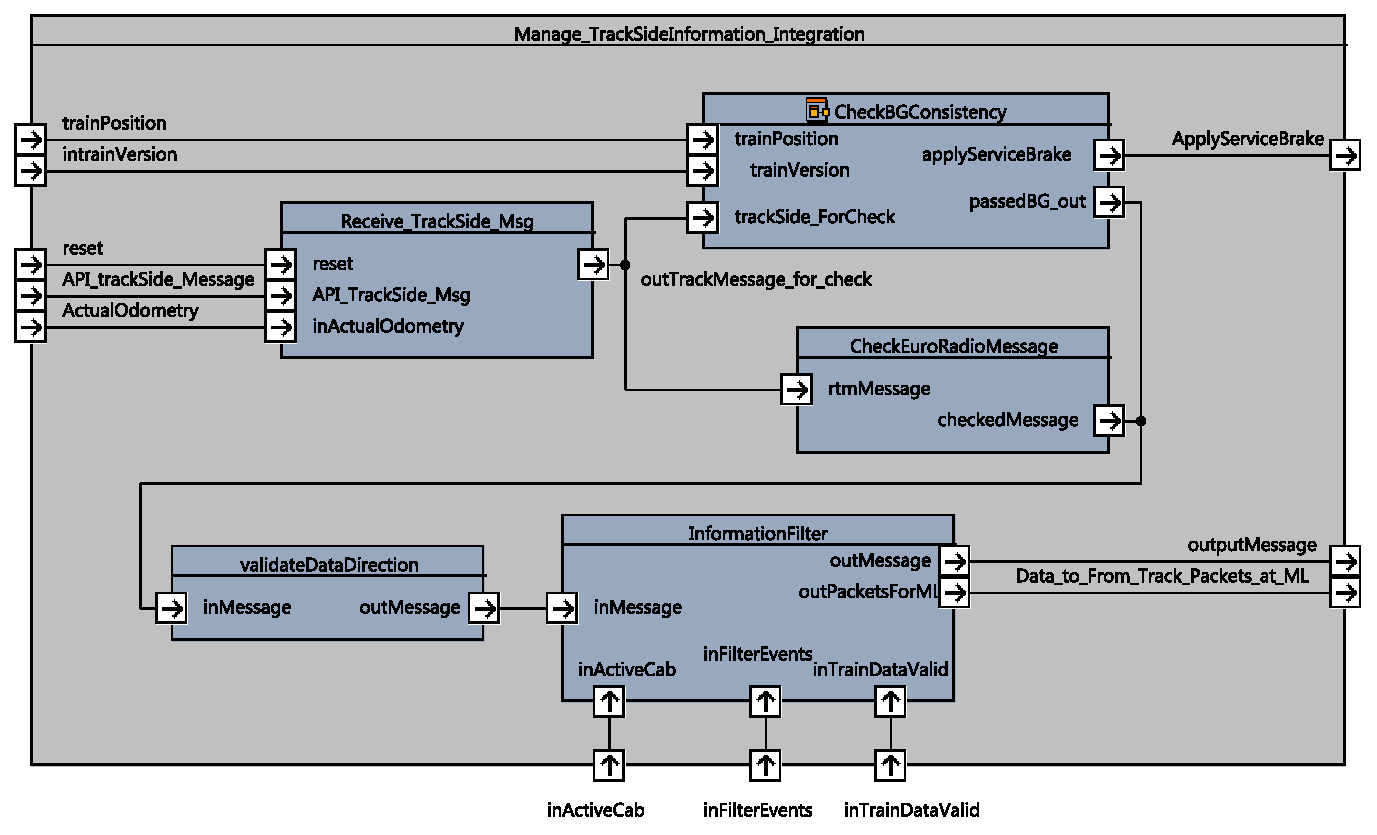
\includegraphics[width=\textwidth]{./images/F2_1_Manage_Trackside_Information_Integration_SysML.pdf}
\caption{Manage\_TrackSideInformation\_Integration component SysML diagram.}\label{f:receiveAndCheckConsistencyArch}
\end{figure}


\subsubsection{Inputs}\label{s:Manage_Trackside_inputs}

\paragraph{fullChecks}

\begin{longtable}{p{.25\textwidth}p{.7\textwidth}}
\toprule
Input name				& fullChecks \\
\midrule
Description				& Indicates, if all checks on the message should be performed. This parameter is for testing purposes only and has to be replaced by a constant in real operation.\\
\midrule
Source					& This item is only relevant in verification phases. In a real system checks are always activated. \\ 
\midrule
Type					& bool \\
\midrule
Valid range of values	& 
\begin{description}
\item[true] All checks are performed.
\item[false] Component InformationFilter is deactivated.
\end{description} \\
\midrule
Behaviour when value is at boundary	& n/a \\
\midrule
Behaviour for values out of valid range	& n/a \\
\midrule
Behaviour when value is erroneous, absent or unwanted (i.e. spurious) & n/a\\
\bottomrule
\end{longtable}


\paragraph{API\_trackSide\_Message}

\begin{longtable}{p{.25\textwidth}p{.7\textwidth}}
\toprule
Input name				& API\_trackSide\_Message \\
\midrule
Description				& Track side message received from the API. The API performs preprocessing of RTM and BTM messages and delivers a maximum of a single message per cycle. The structure of this message is defined in the API [BTM] and [EURORADIO] sections. The input consists of the following main components:\\
&
\begin{description}
\item[valid](bool) Indicates the information has been refreshed in the cycle.
\begin{description}
\item[true]: Information is updated in this cycle.
\item[false]: Information is unchanged.
\end{description}
\end{description}\\
&
\begin{description}
\item[systemTimeMsgReceived](Obu\_BasicTypes\_Pkg::T\_internal\_Type): Timestamp when the system (i.e. the train) has received the message. The parameter is set either by RTM or by BTM modules.
\end{description}\\
&
\begin{description}
\item[msg\_type](Common\_Types\_Pkg::MsgSource\_T) source of this information. 
\begin{description}
\item[msrc\_undefined] indicates the information is not defined. This input is expected when valid flag is false.
\item[msrc\_Euroradio] indicates the information is a euroradio message.
\item[msrc\_Eurobalise] indicates the information is a balise telegram.
\end{description}
Other values of this enumeration are not expected in this model.
\end{description}\\
&
\begin{description}
\item[btm\_msg](API\_Msg\_Pkg::API\_TelegramHeader\_T) Telegram header with some additional information provided by the btm-module. The header is structured as follows:
\begin{description}
\item[present](bool) Telegram information has been received via BTM and the information of this telegram is present. 
\item[checkResult](bool) The telegram is checked after reception at the BTM. Typical checks are checksum-tests or checks at conversion of the types from bit-layout to the presentation in the evc. If checkResult is false the information may not be used. The information is evaluated in the checkBGConsistency component of this model.
\item[api\_bad\_balise\_received](bool) The telegram reception was disturbed. Again, the information related to this telegram may not be used in the EVC.
\item[api\_header](API\_Msg\_Pkg::API\_TelegramHeader\_T) Header of the telegram similar to Subset 026, Section 8.4.2.1. The information in the telegram is not packed on bit-boundaries.
\item[centerOfBalisePosition](BG\_Types\_Pkg::\newline centerOfBalisePosition\_T) Location of the balise as determined by the antenna of the train. The information is extended with inaccuracies of the measurement given by the BTM.
\end{description}
\end{description}\\
&
\begin{description}
\item[rtm\_msg](API\_Msg\_Pkg::API\_RadioMsgHeader\_T) Radio message header with some additional information added by the RTM module. The information is structured as follows:
\begin{description}
\item[present](bool) Radio message has been received via rtm and the information of this message is present. 
\item[apiConsistencyError](bool) The message is checked after reception at the btm. Typical checks are checksum-tests or checks at conversion of the types from bit-layout to the presentation in the evc. If apiConsistencyError is false the information may not be used. The information is evaluated in the checkRadioMessage component of this model.
\item[Radio\_Common\_Header](Radio\_Types\_Pkg::\newline Radio\_TrackTrain\_Header\_T) Header of the radio-message as defined in Subset-026, Section 8.4.4.6.1. In the SRS, depending on the concrete message, some optional variables are defined. In our implementation all optional variables are foreseen. In order to indicate the availability of variables the component radioMetadata is used (see below).
\item[radioMetadata](Common\_Types\_Pkg::RadioMetadata\_T) Metadata for optional variables in the common radio message header. For each optional component a presence indicator of type bool is in the list.  
\item[sendingRBC\_Id](Common\_Types\_Pkg::RBC\_Id\_T) Identifies the RBC as it is known at the RTM. Information is added to the interface in the RTM.
\begin{description}
\item[packets](Common\_Types\_Pkg::CompressedPackets\_T) Packets as received as a part of the telegram or radio message. The structure is set-up and can be accessed by library routines of the trackMessages component of the system. In the manage\_trackside\_Messages component packets may be changed to being absent (e.g., by the function validateDataDirection or by the InformationFilter.). If packets have to be treated only this valid indicator is changed. No other parts of the packets are accessed.
\end{description}
\end{description}
\end{description}
\\
\midrule
Source					& F2 input API\_fromTrack 
\\ 
\midrule
Type					& API\_Msg\_Pkg::API\_TrackSideInput\_T \\
\midrule
Valid range of values	& Access to the information has to be guarded by the valid flag and similar flags deeper in the structure of the interface. Checks on individual values of message components, telegrams and packets are part of the decoding function. We assume information to be valid in this part of the system.\\
\midrule
Behaviour when value is at boundary	& n/a (structure)\\
\midrule
Behaviour for values out of valid range	& n/a\\
\midrule
Behaviour when value is erroneous, absent or unwanted (i.e. spurious) &n/a\\
\bottomrule
\end{longtable}


\paragraph{ActualOdometry}

\begin{longtable}{p{.25\textwidth}p{.7\textwidth}}
\toprule
Input name				& ActualOdometry \\
\midrule
Description				& Odometry data provided by the external odometry module of the train. It contains relative location information with inaccuracies. In this model only information related to the position of the train is used (ODO component). A valid flag of the odometer input indicates the hardware is working and the parameter may be used.\\
\midrule
Source					& F2 input API\_Odometery \\ 
\midrule
Type					& Obu\_BasicTypes\_Pkg::odometry\_T \\
\midrule
Valid range of values	& From the ODO component the nominal position is used. No plausibility checks on the component are done. Any integer value is allowed. \\
\midrule
Behaviour when value is at boundary	& Boundary value may lead to jump of the calculation in negative ranges. As a result the train may not being able to complete the reading of a balise group. In consequence, this results in a balise group error and in a service brake reaction of the train.\\
\midrule
Behaviour for values out of valid range	& Same as description at boundary.\\
\midrule
Behaviour when value is erroneous, absent or unwanted (i.e. spurious) & Same as description at boundary.\\

\bottomrule
\end{longtable}

\paragraph{reset}

\begin{longtable}{p{.25\textwidth}p{.7\textwidth}}
\toprule
Input name				& reset \\
\midrule
Description				& The reset input is used to delete all data stored in the module (e.g.~collected balise telegrams, which do not yet form a complete message). If the input is set to true, all data kept in the module is deleted and no input is accepted. The reset option is to be used when the EVC is started or in system error scenarios.\\
\midrule
Source					& F2 input EVC\_reset
\\ \midrule
Type					& bool \\
\midrule
Valid range of values	& 
\begin{description}
\item[true] All data kept in the module is deleted and no input is accepted.
\item[false] No action. Data at input is accepted.
\end{description} \\
\midrule
Behaviour when value is at boundary	& n/a\\
\midrule
Behaviour for values out of valid range	& n/a\\
\midrule
Behaviour when value is erroneous, absent or unwanted (i.e. spurious) & n/a\\
\bottomrule
\end{longtable}
\newpage
\paragraph{trainPosition}

\begin{longtable}{p{.25\textwidth}p{.7\textwidth}}
\toprule
Input name				& trainPosition \\
\midrule
Description				& Contains the current position of the train. This input is used for validation of the direction of packets and for checks of balise groups. Most important information in this input is the LRBG and the prevLRBG component. This identifies the last two balise group passed by the train.\\
\midrule
Source					& F2.6 calculateTrainPosition \\ 
\midrule
Type					& TrainPosition\_Types\_Pck::trainPosition\_T \\
\midrule
Valid range of values	& A valid flag is used in this input to indicate data is provided correctly.\\
\midrule
Behaviour when value is at boundary	& n/a\\
\midrule
Behaviour for values out of valid range	& n/a\\
\midrule
Behaviour when value is erroneous, absent or unwanted (i.e. spurious) & n/a\\
\bottomrule
\end{longtable}

\paragraph{modeAndLevel}

\begin{longtable}{p{.25\textwidth}p{.7\textwidth}}
\toprule
Input name				& modeAndLevel \\
\midrule
Description				& Provides the current level and mode of the EVC. Mode and Level are used by the InformationFilter subcomponent.\\
\midrule
Source					& F2.5 ManageLevelAndMode \\ 
\midrule
Type					& BG\_Types\_Pkg::ModeAndLevelStatus\_T \\
\midrule
Valid range of values	& n/a\\
\midrule
Behaviour when value is at boundary	& n/a\\
\midrule
Behaviour for values out of valid range	& n/a\\
\midrule
Behaviour when value is erroneous, absent or unwanted (i.e. spurious) & n/a\\
\bottomrule
\end{longtable}


\paragraph{tNvContact}

\begin{longtable}{p{.25\textwidth}p{.7\textwidth}}
\toprule
Input name				& tNvContact \\
\midrule
Description				& For monitoring the safe radio connection, this national value is needed as an input. This parameter is used in the radioCheck component of this model. \\
\midrule
Source					& F2 input API\_persistentData\\ 
\midrule
Type					& Obu\_BasicTypes\_Pkg::T\_internal\_Type \\
\midrule
Valid range of values	& Positive integer. \\
\midrule
Behaviour when value is at boundary	& When boundary is reached the input will jump to 0.\\
\midrule
Behaviour for values out of valid range	& If negative, this parameter will result in a radio message sequence error. Connection to the rbc will be closed.\\
\midrule
Behaviour when value is erroneous, absent or unwanted (i.e. spurious) & See above.\\
\bottomrule
\end{longtable}

\paragraph{intrainVersion}

\begin{longtable}{p{.25\textwidth}p{.7\textwidth}}
\toprule
Input name				& intrainVersion \\
\midrule
Description				& For monitoring the safe radio connection, this national value is needed as an input. This parameter is used in the radioCheck component of this model. \\
\midrule
Source					& F2 input API\_persistentData\\ 
\midrule
Type					& M\_VERSION \\
\midrule
Valid range of values	& Enumerated values.\\
\midrule
Behaviour when value is at boundary	& Value check will reject radio message resp. balise telegram. In the consequence train will stop respectively the session will be rejected. \\
\midrule
Behaviour for values out of valid range	& Value check will reject radio message resp. balise telegram. In the consequence train will stop respectively the session will be rejected.\\
\midrule
Behaviour when value is erroneous, absent or unwanted (i.e. spurious) & See above. \\
\bottomrule
\end{longtable}


\paragraph{lastRelevantEventTimestamp}

\begin{longtable}{p{.25\textwidth}p{.7\textwidth}}
\toprule
Input name				& lastRelevantEventTimestamp \\
\midrule
Description				& For monitoring the safe radio connection, it is necessary that the time between two packets is less than the value of {T\_NVCONTACT}.\newline
In situations like level changes or announced radio holes, not the timestamp of the last message is relevant for comparison, but the timestamp of the last relevant event. This can for example be the timestamp of the level change or the timestamp of the moment, when the train was passing the end of the radiohole.

For performing this check, the timestamp of the last relevant event is provided to the model as an {T\_internal\_Type}-type. \\
\midrule
Source					& F2.1 Manage\_TracksideInformation\_Integration\\ 
\midrule
Type					& Obu\_BasicTypes\_Pkg::T\_internal\_Type \\
\midrule
Valid range of values	& Positive integer.\\
\midrule
Behaviour when value is at boundary	& Once the largest possible timestamp is exceeded, the next timestamps will start from 0 again. This may result in calculations of durations with negative result. As a consequence, the train will react with the loss of the communication session.\\
\midrule
Behaviour for values out of valid range	& See above.\\
\midrule
Behaviour when value is erroneous, absent or unwanted (i.e. spurious) & See above.\\
\bottomrule
\end{longtable}


\paragraph{connectionStatus}

\begin{longtable}{p{.25\textwidth}p{.7\textwidth}}
\toprule
Input name				& connectionStatus \\
\midrule
Description				& Status information about the radio connection. The information is needed to perform the timing check, which depends on the connection state in the radioCheck component. \\
\midrule
Source					& F2.9 MoRC\_Main \\ 
\midrule
Type					& Radio\_Types\_Pkg::sessionStatus\_Type \\
\midrule
Valid range of values	& 
\begin{description}
\item[DISCONNECTED] The OBU is currently not connected to a RBC.
\item[CONNECTING] The OBU is currently connecting to the RBC. Received messages belong to the process of establishing a connection.
\item[CONNECTION\_ESTABLISHED] The connection to the RBC is established.
\end{description} \\
\midrule
Behaviour when value is at boundary	& n/a\\
\midrule
Behaviour for values out of valid range	& n/a\\
\midrule
Behaviour when value is erroneous, absent or unwanted (i.e. spurious) & n/a\\
\bottomrule
\end{longtable}


\paragraph{inSupervisingRbcId}

\begin{longtable}{p{.25\textwidth}p{.7\textwidth}}
\toprule
Input name				& inSupervisingRbcId \\
\midrule
Description				& For the InformationFilter subcomponent, the information which radio messages are sent by the supervising RBC is needed. To recognize these messages, the identifier of the supervising RBC is needed. \\
\midrule
Source					& F2.9 MoRC\_Main\\ 
\midrule
Type					& int \\
\midrule
Valid range of values	& 0, 1, 2
 \\
\midrule
Behaviour when value is at boundary	& n/a\\
\midrule
Behaviour for values out of valid range	&  Is interpreted as non valid radio connection.\\
\midrule
Behaviour when value is erroneous, absent or unwanted (i.e. spurious) & Is interpreted as non valid radio connection.\\
\bottomrule
\end{longtable}


\paragraph{inAnnouncedBGs}

\begin{longtable}{p{.25\textwidth}p{.7\textwidth}}
\toprule
Input name				& inAnnouncedBGs \\
\midrule
Description				& Provides information about balise groups as known in the EVC. This information is generated by the CalculateTrainPosition component based on the linking information received from track side and on the balise groups passed by the train.\\
\midrule
Source					& F2.6 calculateTrainPosition \\ 
\midrule
Type					& TrainPosition\_Types\_Pck::positionedBGs\_T \\
\midrule
Valid range of values	& Each balise group netry is identified by an valid flag. \\
\midrule
Behaviour when value is at boundary	& n/a\\
\midrule
Behaviour for values out of valid range	& n/a\\
\midrule
Behaviour when value is erroneous, absent or unwanted (i.e. spurious) & n/a\\
\bottomrule
\end{longtable}


\paragraph{q\_nvlocacc}

\begin{longtable}{p{.25\textwidth}p{.7\textwidth}}
\toprule
Input name				& q\_nvlocacc \\
\midrule
Description				& This national value determines the location accuracy. Needed as input for checkBGConsistency.  \\
\midrule
Source					& F2 input API\_persistentData\\ 
\midrule
Type					& Q\_NVLOCACC \\
\midrule
Valid range of values	& Integers in the range 0, \ldots, 63\\
\midrule
Behaviour when value is at boundary	& No impact.\\
\midrule
Behaviour for values out of valid range	& Will result in wrong calculation of inaccuracy of the train.\\
\midrule
Behaviour when value is erroneous, absent or unwanted (i.e. spurious) & See above.\\
\bottomrule
\end{longtable}


\paragraph{inActiveCab}

\begin{longtable}{p{.25\textwidth}p{.7\textwidth}}
\toprule
Input name				& inActiveCab \\
\midrule
Description				& Indicates the cab is active. This input is used by the InformationFilter subcomponent. \\
\midrule
Source					& F2.12 manageTIU\_input\\ 
\midrule
Type					& bool\\
\midrule
Valid range of values	& 
\begin{description}
\item[true] Cab is active.
\item[false] Cab is inactive.
\end{description}\\
\midrule
Behaviour when value is at boundary	& n/a\\
\midrule
Behaviour for values out of valid range	& n/a\\
\midrule
Behaviour when value is erroneous, absent or unwanted (i.e. spurious) & n/a\\
\bottomrule
\end{longtable}

\paragraph{inTrainDataValid}

\begin{longtable}{p{.25\textwidth}p{.7\textwidth}}
\toprule
Input name			& inTrainDataValid \\
\midrule
Description			& Indicates train data have been validated by the RBC. This input is used by the InformationFilter subcomponent. \\
\midrule
Source				& F2.3 trainData\\ 
\midrule
Type				& bool \\
\midrule
Valid range of values		& 
\begin{description}
\item[true] Train data has been validated.
\item[false] Train data has not been validated.
\end{description}\\
\midrule
Behaviour when value is at boundary	& n/a\\
\midrule
Behaviour for values out of valid range	& n/a\\
\midrule
Behaviour when value is erroneous, absent or unwanted (i.e. spurious) & n/a\\
\bottomrule
\end{longtable}

\paragraph{inFilterEvents}

\begin{longtable}{p{.25\textwidth}p{.7\textwidth}}
\toprule
Input name			& inFilterEvents \\
\midrule
Description			& A set of events needed for controlling the InformationFilter subcomponent. For details see valid range of values row in this table.\\
\midrule
Source				& F2.3 trainData
%ModeAndLevels, MoRC
\\  
\midrule
Type					& Common\_Types\_Pkg::filterRelatedEvents\_T\\
\midrule
Valid range of values	& This input is a complex structure consisting out of the following components:
\begin{description}
\item[pendingL1Transition](bool) Indicates if an announced LEVEL 1 transition is present. Used for Level filter exception [1]. The information is indicating the status.
Note: this indication can be evaluated based on information available in the InformationFilter. The input is not used from outside the main component Manage\_TrackSide\_Information.
\item[pendingL2L3Transition](bool) Indicates if an announced LEVEL 2 or Level 3 transition is present. Used for Level Filter exception [2]. The information is indicating the status.
Note: this indication can be evaluated based on information available in the InformationFilter. The input is not used from outside the main component Manage\_TrackSide\_Information.
\item[pendingAckOfTrainDataFromRBC](bool) Indicates if the acknowledgement of train data is pending. Used for Level filter exception [3].
\item[emergencyStopAccepted](bool): Indicate if the train performs an emergency brake. Used for Level filter exception [5].
\item[lastAckTextMessageId](int) The ID of the last acknowledged text message ID. Used for Level filter exception [12]. The SRS requires text messages to restrict from double sending to the DMI when handled in the filter. This function is currently not implemented. 
\item[pendingNTCTransition](bool) Indication if an announced LEVEL NTC transition is present. Used for Level filter exception [6,7].
\item[SPPAndGradientOnBoard](bool) Speed Profile and Gradient Profile received and available on board. This information may be part of the actual incoming message.
\item[MACoverNotFullLength](bool) MA does not cover full length of the trip. Information from trackAtlas.
\end{description}\\
\midrule
Behaviour when value is at boundary	& n/a\\
\midrule
Behaviour for values out of valid range	& n/a\\
\midrule
Behaviour when value is erroneous, absent or unwanted (i.e. spurious) & n/a\\
\bottomrule
\end{longtable}

\paragraph{transitionPositionPassed}

\begin{longtable}{p{.25\textwidth}p{.7\textwidth}}
\toprule
Input name				& transitionPositionPassed \\
\midrule
Description				& The position of the requested level transition has been passed. This information is used by InformationFilter subcomponent to clean data after level management reactions.
\\
\midrule
Source					& F2.5 ManageLevelAndMode\\ 
\midrule
Type					& bool\\
\midrule
Valid range of values	& 
\begin{description}
\item[true] The position of the requested level transition has been passed.
\item[false] The position of the requested level transition has not been passed.
\end{description}\\
\midrule
Behaviour when value is at boundary	& n/a\\
\midrule
Behaviour for values out of valid range	& n/a\\
\midrule
Behaviour when value is erroneous, absent or unwanted (i.e. spurious) & n/a\\
\bottomrule
\end{longtable}



\subsubsection{Outputs}\label{s:Manage_Trackside_outputs}

\paragraph{outputMessage}

\begin{longtable}{p{.25\textwidth}p{.7\textwidth}}
\toprule
Output name				& outputMessage \\
\midrule
Description				& Combines both balise and radio messages to one common datatype. This datatype contains all variables and packets, which are possible for the given scenario. In each cycle at most one valid message is put to the output. The InformationFilter subcomponent might take the last processed one or a message from stack - depending on the information stored and on the status of the evc. The component consists of the following building blocks:\\
&
\begin{description}
\item[valid] Information about the status of this message.
\begin{description}
\item[true] The information is valid, a new message is now visible at the output. The valid flag (and the message as such) will only be present for one cycle.
\item[false] No valid message is available.
\end{description}
\end{description}\\
&
\begin{description}
\item[source](Common\_Types\_Pkg::MsgSource\_T) Source of this information. 
\begin{description}
\item[msrc\_undefined] Indicates the information is not defined. This input is expected when valid flag is false.
\item[msrc\_Euroradio] Indicates the information is a euroradio message.
\item[msrc\_Eurobalise] Indicates the information is a balise telegram.
\end{description}
Other values of this enumeration are not expected in this model.
\item[radioMetadata](Common\_Types\_Pkg::RadioMetadata\_T) Metadata for optional variables in the common radio message header. For each optional component a presence indicator of type bool is in the list.  
\item[BG\_Common\_Header](BG\_Types\_Pkg::BG\_Header\_T) Balise group message header with some additional information. This header collects information from the balise telegram headers together with the location and orientation of the balise group related to the driving direction.

\item[Radio\_Common\_Header](Radio\_Types\_Pkg::\newline Radio\_TrackTrain\_Header\_T) Radio message header with some additional information added by the RTM module. Variables of messages which are not present in all messages are available in the header, but controlled by the radio metadata.
\item[packets](Common\_Types\_Pkg::CompressedPackets\_T) Packets as received as a part of the telegram or radio message. The structure is set-up and can be accessed by library routines of the trackMessages component of the system. In the manage\_trackside\_Messages component packets my be changed to being absent (e.g., by the function validateDataDirection or by the InformationFilter.). If packets have to be treated only this valid indicator is changed. No other parts of the packets are changed.
\end{description}
\\
\midrule
Destination				& F2.4 TrackAtlas\newline
F2.6 calculateTrainPosition\newline
F2.8 ProvidePositionReport\newline
F2.9 MoRC\_Main
\\ 
\midrule
Type					& Common\_Types\_Pkg::ReceivedMessage\_T \\
\midrule
Valid range of values	& n/a\\
\midrule
Behaviour when value is at boundary	& n/a\\
\midrule
Behaviour for values out of valid range	& n/a\\
\midrule
Behaviour when value is erroneous, absent or unwanted (i.e. spurious) & n/a\\
\bottomrule
\end{longtable}


\paragraph{ApplyServiceBrake}

\begin{longtable}{p{.25\textwidth}p{.7\textwidth}}
\toprule
Output name				& ApplyServiceBrake \\
\midrule
Description				&  Indicates if the balise group the train just passed could not be processed correctly. The check results in the request for a service break. \\
\midrule
Destination				& F2.7 SpeedSupervision\_Integration\\ 
\midrule
Type					& bool \\
\midrule
Valid range of values	& 
\begin{description}
\item[true] Request for service break.
\item[false] No request for service break.
\end{description}\\
\midrule
Behaviour when value is at boundary	& n/a\\
\midrule
Behaviour for values out of valid range	& n/a\\
\midrule
Behaviour when value is erroneous, absent or unwanted (i.e. spurious) & n/a\\
\bottomrule
\end{longtable}


\paragraph{BadBaliseMessageToDMI}

\begin{longtable}{p{.25\textwidth}p{.7\textwidth}}
\toprule
Output name				& BadBaliseMessageToDMI \\
\midrule
Description				& Information to be passed to the DMI to indicate the reception of a ``bad balise'' to the driver. \\
\midrule
Destination				& F2.11 manageDMI\_output
\\
\midrule
Type					& bool \\
\midrule
Valid range of values	& 
\begin{description}
\item[true] Reception of ``bad balise'' should be indicated to the driver.
\item[false] Reception of ``bad balise'' should not be indicated to the driver.
\end{description}\\
\midrule
Behaviour when value is at boundary	& n/a\\
\midrule
Behaviour for values out of valid range	&  n/a\\
\midrule
Behaviour when value is erroneous, absent or unwanted (i.e. spurious) &  n/a\\
\bottomrule
\end{longtable}


\paragraph{outCheckErrors}

\begin{longtable}{p{.25\textwidth}p{.7\textwidth}}
\toprule
Output name				& outCheckErrors \\
\midrule
Description				& Error flags for errors found during the message check procedures. For details see valid range of values row of this table.\\
\midrule
Destination				& F2.5 ManageModeAndLevel\newline
F2.8 ProvidePositionReport\\ 
\midrule
Type					& Common\_Types\_Pkg::MSG\_Errors\_T\\
\midrule
Valid range of values	& This output is a complex structure mainly consisting out of boolean values. The boolean variables are set true if an error in the particular parameter has been detected and false otherwise.
\begin{description}
\item[linkedBGError](bool) Reported by checkBGConsistency. Error in a linked BGH - Message has been detected.
\item[unlinkedBGError](bool) Reported by checkBGConsistency. Error in an unlinked BGH - Message has been detected.
\item[BG\_versionIncompatible](bool) Reported by checkBGConsistency. Version of received Balises is not compliant with the train. Balises cannot be used.
\item[radioSequenceError](bool) Reported by checkEuroRadioMessage. The sequence of messages in the input channel is not correct. This check is based in t\_train of the incoming radio messages.
\item[tNvContactError](bool) Reported by checkEuroRadioMessage. The time for receiving the next radio message has been exceeded. This indicates lost radio messages.
\item[otherTimingError](bool) Reported by checkEuroRadioMessage. Other timing errors.
\item[radioMessageConsistencyError](bool) Reported by checkEuroRadioMessage. Inconsistencies in the contents of radio messages have been detected.
\item[nid\_c](NID\_C) Reported by checkBGConsistency. If known id of the erroneous balise group.
\item[nid\_errorbg](NID\_ERRORBG) Reported by checkBGConsistency. If known id of the erroneous balise group.
\end{description}
\\
\midrule
Behaviour when value is at boundary	& n/a\\
\midrule
Behaviour for values out of valid range	& n/a\\
\midrule
Behaviour when value is erroneous, absent or unwanted (i.e. spurious) & n/a\\
\bottomrule
\end{longtable}


\paragraph{forLevelManagement}

\begin{longtable}{p{.25\textwidth}p{.7\textwidth}}
\toprule
Output name				& forLevelManagement \\
\midrule
Description				& The InformationFilter subcomponent has to provide information to the EVC components according to the actual level and radio state. In order to trigger the level change level management needs to know about avaialblity of track profiles and other components in order to select the correct mode and level. This output provides information relevant to trigger level transitions. The data will be accumulated in the InformationFilter until the position for the level change has been reached. The output structure consists of the following components:
\begin{description}
\item[P41](Packet\_Types\_Pkg::P41\_LevelTransistionOrders\_T) Packet 41 (level transition order). 
\item[P46](Packet\_Types\_Pkg::P46\_LevelTransistionOrders\_T) Packet 46 (conditional level transition order). 
\item[LRBG](NID\_LRBG) Reference LRBG for the level transition order..
\item[referenceLocation](Obu\_BasicTypes\_Pkg::L\_internal\_Type) Location of the reference LRBG. This location has to be used as reference for calculating the level transition position. 
\item[P12\_received](bool) Packet 12 (Level 1 Movement Authority) has been received at the InfomationFilter subcomponent in the context of this level transition. 
\item[P15\_received](bool) Packet 15 (Level 2/3 Movement Authority) has been received at the InfomationFilter subcomponent in the context of this level transition. 
\item[P21\_received](bool) Packet 21 Gradient Profile) has been received at the InfomationFilter subcomponent in the context of this level transition. 
\item[P27\_received](bool) Packet 27 (International Static Speed Profile) has been received at the InfomationFilter subcomponent in the context of this level transition. 
\end{description}

\\
\midrule
Destination				& F2.5 ModesAndLevels
\\ 
\midrule
Type					& Level\_And\_Mode\_Types\_Pkg::T\_Data\_From\_TrackForLevelChange\\
\midrule
Valid range of values	& \begin{description}
\item[true] An error in a unlinked balise group was detected.
\item[false] No error in a unlinked balise group was detected.
\end{description} \\
\midrule
Behaviour when value is at boundary	& n/a\\
\midrule
Behaviour for values out of valid range	& n/a\\
\midrule
Behaviour when value is erroneous, absent or unwanted (i.e. spurious) & n/a\\
\bottomrule
\end{longtable}


\paragraph{outputMessageForRadioAck}

\begin{longtable}{p{.25\textwidth}p{.7\textwidth}}
\toprule
Output name				& outputMessageForRadioAck \\
\midrule
Description				& Even if an imcoming radio message is rejected or kept for some time in the buffer of the InformationFilter subcomponent, some information needs to be made available for maintaining the communication session with the RBC, e.g., the timestamp of the received message and acknowledgment of message reception based on the ACK flag. No other information of this message is to be used in the EVC. This concept might be improved when radio management functions are rearranged.
\\
\midrule
Destination				& F2.3 trainData\\ 
\midrule
Type					& Common\_Types\_Pkg::ReceivedMessage\_T \\
\midrule
Valid range of values	& \begin{description}
\item[true] An error in a unlinked balise group was detected.
\item[false] No error in a unlinked balise group was detected.
\end{description} \\
\midrule
Behaviour when value is at boundary	& n/a\\
\midrule
Behaviour for values out of valid range	& n/a\\
\midrule
Behaviour when value is erroneous, absent or unwanted (i.e. spurious) & n/a\\
\bottomrule
\end{longtable}

% Description of sub components
\subsection{Subcomponents}\label{s:receivetrackdata_subcomponents}

\subsubsection{Receive\_TrackSide\_Msg}
%set the master document for easy compilation
%!TEX root = ../D3_5_3.tex

\paragraph{Component Requirements}
\begin{longtable}{p{.25\textwidth}p{.7\textwidth}}
\toprule
Component name			& Receive\_TrackSide\_Msg \\
\midrule
Link to SCADE model		& {\footnotesize \url{https://github.com/openETCS/modeling/tree/master/model/Scade/System/ObuFunctions/ManageLocationRelatedInformation/BaliseGroup/Receive_TrackSide_Msg}} \\
\midrule
SCADE designer			& Bernd Hekele, DB Netz AG \\
\midrule
Description				& This function defines the interface of the OBU model to the openETCS generic API for Eurobalise  and Euroradio messages. On the interface, either a valid telegram/message is provided or a telegram/message is indicated which could not be received correct when passing the balise or receiving the radio message. The function passes a balise telegram without major changes of the information to the next entity for collecting the balise group information. This entity collects telegrams received via the interface into Balise Group Information. In case of a radio message, the message is converted to an internal format for further processing and passed without changing the information contained.
\begin{itemize}
\item The decoding of balises is done at the API. Also, packets received via the interface are already transformed into a usable shape.
\item Only packets used inside the current model are passed via the interface.
\item Treatment of Packet 5: Linking Information.
Linking Information is added to the linking array starting from index 0 without gaps. Used elements are marked as valid. Elements are sorted according to the order given by the telegram sequence.
\item Telegrams received as invalid are passed to the ``Check-Function'' to process errors in communication with the track side according to the requirements and in a single place.
Telegrams are added to the telegram array starting from index 0 without gaps. Used elements are marked as valid. Elements are stored according to the order given by the telegram sequence.
\item This function does not process information from the packets. The information is passed to the check without further processing of the values. 
\end{itemize} \\
\midrule
Input documents	&
  Subset-026, Chapter 7 and 8: Definition of the Balise Telegram\newline
  Subset-026, Chapter 4.2.2, 4.2.4, 4.2.9: Interface to the BTM\newline
  Subset-026, Chapter 3.4.1 - 3.4.3, 3.16.2: Handling of Balise Telegrams\newline
  Subset-026, Chapter 3.16.2: Check of the balise group\newline
  Subset-026, Chapter 3.4.2: Determining the orientation\newline
  Subset-026, Chapter 4.5.2: Active Functions Table\newline
  Subset-026, Chapter 8.4.4: Rules for Euroradio messages \\
\midrule
Safety integrity level		& 4 \\
\midrule
Time constraints		& n/a \\
\midrule
API requirements 		& n/a \\
\bottomrule
\end{longtable}


\paragraph{Interface}

For an overview of the interface of this internal component we refer to the SCADE model (cf.~link above) respectively the SCADE generated documentation.

\subsubsection{CheckBGConsistency}
%set the master document for easy compilation
%!TEX root = ../D3_5_3.tex

\paragraph{Component Requirements}

\begin{longtable}{p{.25\textwidth}p{.7\textwidth}}
\toprule
Component name			& CheckBGConsistency \\
\midrule
Link to SCADE model		& {\footnotesize \url{https://github.com/openETCS/modeling/tree/master/model/Scade/System/ObuFunctions/ManageLocationRelatedInformation/BaliseGroup/CheckBGConsistency}} \\
\midrule
SCADE designer			& Peyman Farhangi, DB Netz AG \\
\midrule
Description				& The function "Receive\_TrackSide\_Msg" collects the telegrams in an
array. If one or more telegrams are received multiple times, either the whole array or single telegram should be deleted.(e.g.if the train moves back.) The balises in a group are to be expected in a certain distance from each other. The function "Receive\_TrackSide\_Msg" checks if the telegrams has been received in due time and at the right expected location.
\\
&
The function "CheckBGConsistency" verifies the completeness and correctness of the received telegrams from balise groups and composes the balise message from the received telegram array (input from "Receive\_TrackSide\_Msg"). A balise message is built from at least one telegram and a maximum of 8 telegrams. When linking information is used on-board, only balise groups marked as linked and included in the linking information and balise groups marked as unlinked shall be taken into account.
\\
&
\begin{itemize}
\item A message is still complete and correct, if a telegram is missing (or not decoded or incompletely decoded), and this telegram is duplicated within the balise group and the duplicating one is correctly read.

\item In case of multiple telegrams, the order of N\_PIG of telegrams must be either ascending (nominal) or descending (reverse). And the all telegrams must have the same NID\_BG and NID\_C.

\item A message is not correct, if a message counters (M\_MCOUNT) equals 254 (that means: The telegram never fits any message of the group). A message counter can  equal 255 (that means: The telegram fits with all telegrams of the same balise group) and all other values must be the same.
\end{itemize}

The orientation of the BG and the running direction of the train are calculated in this block.When linking information is used on-board, the check, if the message of linked balise group has been received in due time and at the expected location, will be performed in "Calculate Train Position". The checks on the validity of the data in the packets and the validity with respect to the direction of motion
will be performed in other modules, e.g. "ValidateDataDirection".\\
\midrule
Input documents	& 
Subset-026, Chapter 7 and 8: Definition of the Balise Telegram\newline
Subset-026, Chapter 3.4.1-3, 3.16.2: Handling of Balise Telegrams\newline
Subset-026, Chapter 3.16.2: Check of the balise group\newline
Subset-026, Chapter 4.5.2: Active Functions Table\\
\midrule
Safety integrity level	& 4 \\
\midrule
Time constraints		& n/a \\
\midrule
API requirements 		& n/a \\
\bottomrule
\end{longtable}


\paragraph{Interface}

For an overview of the interface of this internal component we refer to the SCADE model (cf.~link above) respectively the SCADE generated documentation.


\subsubsection{CheckEuroradioMessage}
%set the master document for easy compilation
%!TEX root = ../D3_5_3.tex

\paragraph{Component Requirements}

\begin{longtable}{p{.25\textwidth}p{.7\textwidth}}
\toprule
Component name			& CheckEuroradioMessage \\
\midrule
Link to SCADE model		& {\footnotesize \url{https://github.com/openETCS/modeling/tree/b9c31ce6fdf702b412bbeab3032a8a4dc7c92e5c/model/Scade/System/ObuFunctions/ManageLocationRelatedInformation/BaliseGroup/CheckEuroRadioMessage}} \\
\midrule
SCADE designer			& Stefan Karg, LEA Railergy \\
\midrule
Description				& The component ``CheckEuroradioMessage'' performs consistency and timing checks on the received radio message. These checks are:
\begin{itemize}
 \item Checking the message sequence.
 \item Check if the message violates timing constraints (T\_NVCONTACT).
 \item Check if all mandatory elements are included.
 \item Check if no elements are included, which are forbidden for the given message id.
\end{itemize}
Messages, which violate one or more of these criteria are marked as invalid in the message header and the component signals the reason for the invalidation via different flags as described in the SCADE model. \\
\midrule
Input documents	& 
  Subset-026, Chapter 3.16\newline
  Subset-026, Chapter 8.4.4\\
\midrule
Safety integrity level		& 4 \\
\midrule
Time constraints		& n/a \\
\midrule
API requirements 		& n/a \\
\bottomrule
\end{longtable}


\paragraph{Interface}

For an overview of the interface of this internal component we refer to the SCADE model (cf.~link above) respectively the SCADE generated documentation.

\subsubsection{ValidateDataDirection}
%set the master document for easy compilation
%!TEX root = ../D3_5_3.tex

\paragraph{Component Requirements}

\begin{longtable}{p{.25\textwidth}p{.7\textwidth}}
\toprule
Component name			& ValidateDataDirection \\
\midrule
Link to SCADE model		& {\footnotesize \url{https://github.com/openETCS/modeling/tree/master/model/Scade/System/ObuFunctions/ManageLocationRelatedInformation/BaliseGroup/ValidateDataDirection}} \\
\midrule
SCADE designer			& Stefan Karg, LEA Railergy \\
\midrule
Description				& The component filters an input message in order to mark all elements as invalid, which are not designated for the current driving direction of the train.
\\
&
\begin{itemize}
 \item The operator contains two processing paths for different message types. Radio messages and balise group messages are handeled in a different way. For validating the data direction of a radio message, the check is performed using the balise group referenced in the radio message header as relevant balise group. For balise group message, the LRBG is used.
 \item The metadata of packets, which are recognized as not valid for the current driving direction, is invalidated.
\end{itemize} \\
\midrule
Input documents	& 
  Subset-026, Chapter 3.6.3 \\
\midrule
Safety integrity level	& 4 \\
\midrule
Time constraints		& n/a \\
\midrule
API requirements 		& n/a \\
\bottomrule
\end{longtable}


\paragraph{Interface}

For an overview of the interface of this internal component we refer to the SCADE model (cf.~link above) respectively the SCADE generated documentation.

\subsubsection{InformationFilter}
%set the master document for easy compilation
%!TEX root = ../D3_5_3.tex

\paragraph{Component Requirements}
\todo[inline]{Information filter component description needs to be checked, i.e. is the description still up to date? Should more documentation provided for this component in the ADD (please check with Bernd Hekele)?}

\begin{longtable}{p{.25\textwidth}p{.7\textwidth}}
\toprule
Component name			& InformationFilter \\
\midrule
Link to SCADE model		& {\footnotesize \url{https://github.com/openETCS/modeling/tree/master/model/Scade/System/ObuFunctions/ManageLocationRelatedInformation/BaliseGroup/InformationFilter}} \\
\midrule
SCADE designer			& Christian Stahl, TWT\newline
Alexander Stante, FhG \\
\midrule
Description				& The filter receives track information (balise and radio) and filters them depending of the mode, level and source of the message. Only messages that pass the filter are valid and should be considered by other ETCS subsystems. The filter  consists of four subcomponents: FirstFilter, SecondFilter, ThirdFilter and TransitionBuffer.

\begin{description}
\item[FirstFilter] This filter performs filtering of messages
based on the current ETCS level. The decisions taken process is
described via a big decision table which contains rows for every
packet and columns for every ETCS level. This table encodes also if
certain additional information is necessary to filter a message like
pending ETCS Level transitions. Based on this filter packets of an
incoming message is either rejected, accepted or the whole message is
put in the TransitionBuffer. Messages are put in the TransitionBuffer
if there is an announced level transition and the received message is
only valid for the upcoming level.

\item[SecondFilter] The SecondFilter mainly considers messages
that are received via Euroradio. Certain messages are directly
rejected while other may be stored in the TransitionBuffer. The buffer
is used to store messages that are received from non supervising RBCs,
but will be reevaluated after a RBC transition.

\item[ThirdFilter] The last filter is functionally very similar
the the FirstFilter, however it filters depending on the mode. It also
contains a decision table with rows for every packet but the columns
are modes.

\item[TransitionBuffer] The InformationFilter uses two
TransitionBuffers. One is used to store up to three messages for the
ETCS level transition and the other buffer is used for RBC
transitions. The buffer is designed as a ring buffer and message are
read in FIFO order.
\end{description} \\
\midrule
Input documents	& 
  Subset-026, Chapter 4.8 \\
\midrule
Safety integrity level	& 4 \\
\midrule
Time constraints		& n/a \\
\midrule
API requirements 		& n/a \\
\bottomrule
\end{longtable}


\paragraph{Interface}

For an overview of the interface of this internal component we refer to the SCADE model (cf.~link above) respectively the SCADE generated documentation.


%set the master document for easy compilation
%!TEX root = ../D3_5_3.tex

\section{F2.2: Manage\_ETCS\_Procedures}\label{s:F2.2}

\todo[inline]{Section has to be completed}

\subsection{Component Requirements}

\begin{longtable}{p{.25\textwidth}p{.7\textwidth}}
\toprule
Component name			& Manage\_ETCS\_Procedures \\
\midrule
Link to SCADE model		& {\footnotesize \url{https://github.com/openETCS/modeling/tree/master/model/Scade/System/ObuFunctions/Procedures}} \\
\midrule
SCADE designer			&  Baseliyos Jacob, DB Netz AG\\
\midrule
Description				& This function describes the Start of Mission procedure of the train until the current status will change to another mode, level or other procedure. \\
\midrule
Input documents	& 
Subset-026, Chapter 5.4\\
\midrule
Safety integrity level		& 4 \\
\midrule
Time constraints		& n/a \\
\midrule
API requirements 		& n/a \\
\bottomrule
\end{longtable}


\subsection{Interface}

An overview of the interface of component Manage\_ETCS\_Procedures is shown in Figure~\ref{f:etcs_procedures_interface}. The inputs and outputs are described in detail in Section~\ref{s:etcs_procedures_inputs} respectively \ref{s:etcs_procedures_outputs}. Subcomponents are described in Section~\ref{s:etcs_procedures_subcomponents}.

\begin{figure}
\center
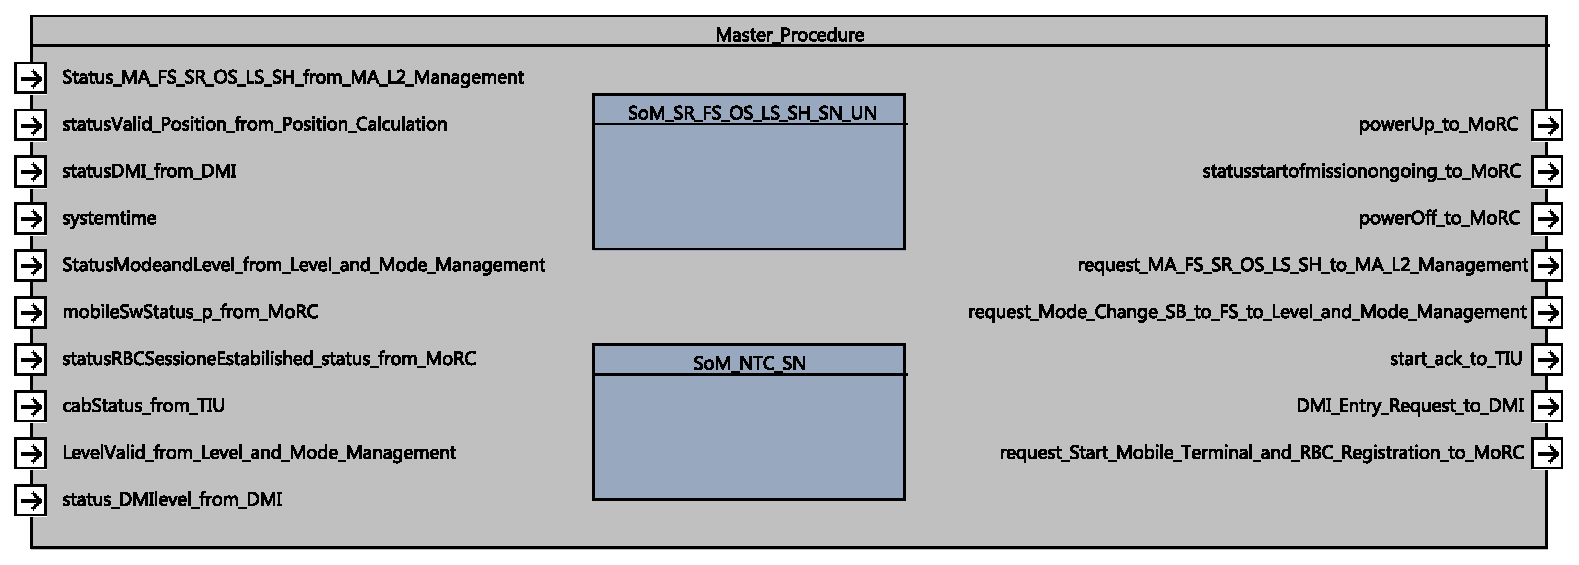
\includegraphics[width=\textwidth]{images/F2_2_Manage_ETCS_Procedures.pdf}
\caption{Manage\_ETCS\_Procedures component SysML diagram.}\label{f:etcs_procedures_interface}
\end{figure}


\subsubsection{Inputs}\label{s:etcs_procedures_inputs}

\paragraph{statusDMI\_from\_DMI}

\begin{longtable}{p{.25\textwidth}p{.7\textwidth}}
\toprule
Input name				& statusDMI\_from\_DMI \\
\midrule
Description				& Input interface of DMI Controller status. \\
\midrule
Source					& F2.10 manageDMI\_input  \\ 
\midrule
Type					& DMI\_Types\_Pkg::DMI\_EVC\_status\_T \\
\midrule
Valid range of values	& \todo[inline]{To be completed} \\
\midrule
Behaviour when value is at boundary	& n/a \\
\midrule
Behaviour for values out of valid range	& Function will not be triggered. \\
\midrule
Behaviour when value is erroneous, absent or unwanted (i.e. spurious) & Function will not be triggered. \\
\bottomrule
\end{longtable}


\paragraph{Status\_MA\_FS\_SR\_OS\_LS\_SH\_from\_MA\_L2\_Management}

\begin{longtable}{p{.25\textwidth}p{.7\textwidth}}
\toprule
Input name				& Status\_MA\_FS\_SR\_OS\_LS\_SH\_from\_MA\_L2\_Management \\
\midrule
Description				& Status of MA, Mode and Level from Level and Mode Management. \\
\midrule
Source					& F2.2 Manage\_ETCS\_Procedures \\ 
\midrule
Type					& bool \\
\midrule
Valid range of values	& \begin{description}
\item[true]Movement Authority for Level 2 FS is valid
\item[false]Movement Authority for Level 2 FS is not valid
\end{description} \\
\midrule
Behaviour when value is at boundary	& n/a \\
\midrule
Behaviour for values out of valid range	& n/a \\
\midrule
Behaviour when value is erroneous, absent or unwanted (i.e. spurious) & n/a \\
\bottomrule
\end{longtable}

\paragraph{systemtime}

\begin{longtable}{p{.25\textwidth}p{.7\textwidth}}
\toprule
Input name				& systemtime \\
\midrule
Description				& Standardized system time used for all internal calculations. \\
\midrule
Source					& F2 input API\_Systemtime \\ 
\midrule
Type					& Obu\_BasicTypes\_Pkg::T\_internal\_Type \\
\midrule
Valid range of values	& 
$[0,\text{maximum positive int value of target platform}]$ \\
\midrule
Behaviour when value is at boundary	& System time is assumed to be valid. \\
\midrule
Behaviour for values out of valid range	& System time is assumed to be valid. \\
\midrule
Behaviour when value is erroneous, absent or unwanted (i.e. spurious) & System time is assumed to be valid. \\
\bottomrule
\end{longtable}

\paragraph{StatusModeandLevel\_from\_Level\_and\_Mode\_Management}

\begin{longtable}{p{.25\textwidth}p{.7\textwidth}}
\toprule
Input name				& StatusModeandLevel\_from\_Level\_and\_Mode\_Management  \\
\midrule
Description				& Status of Mode and Level. \\
\midrule
Source					& F2.10 ManageLevelAndMode \\ 
\midrule
Type					& Level\_And\_Mode\_Types\_Pkg::T\_Mode\_Level \\
\midrule
Valid range of values	& 
\todo[inline]{To be completed} \\
\midrule
Behaviour when value is at boundary	& \todo[inline]{To be completed} \\
\midrule
Behaviour for values out of valid range	& \todo[inline]{To be completed} \\
\midrule
Behaviour when value is erroneous, absent or unwanted (i.e. spurious) & \todo[inline]{To be completed} \\
\bottomrule
\end{longtable}

\paragraph{mobileSwStatus\_p\_from\_MoRC}

\begin{longtable}{p{.25\textwidth}p{.7\textwidth}}
\toprule
Input name				& mobileSwStatus\_p\_from\_MoRC  \\
\midrule
Description				& Information about SW status from Management of Radio Communication function. \\
\midrule
Source					& F2.9 MoRC\_Main\\ 
\midrule
Type					& MoRC\_Pck::mobileSWStatus\_Type \\
\midrule
Valid range of values	& \todo[inline]{To be completed} \\
\midrule
Behaviour when value is at boundary	& \todo[inline]{To be completed} \\
\midrule
Behaviour for values out of valid range	& \todo[inline]{To be completed} \\
\midrule
Behaviour when value is erroneous, absent or unwanted (i.e. spurious) & \todo[inline]{To be completed} \\
\bottomrule
\end{longtable}

\paragraph{statusRBCSessioneEstabilished\_status\_from\_MoRC}

\begin{longtable}{p{.25\textwidth}p{.7\textwidth}}
\toprule
Input name				& statusRBCSessioneEstabilished\_status\_from\_MoRC  \\
\midrule
Description				& Information about RBC Session status from the Management of Radio Communication function. \\
\midrule
Source					&  F2.9 MoRC\_Main\\ 
\midrule
Type					& Radio\_Types\_Pkg::sessionStatus\_Type \\
\midrule
Valid range of values	& \todo[inline]{To be completed} \\
\midrule
Behaviour when value is at boundary	& \todo[inline]{To be completed} \\
\midrule
Behaviour for values out of valid range	& \todo[inline]{To be completed} \\
\midrule
Behaviour when value is erroneous, absent or unwanted (i.e. spurious) & \todo[inline]{To be completed} \\
\bottomrule
\end{longtable}

\paragraph{cabStatus\_from\_TIU}

\begin{longtable}{p{.25\textwidth}p{.7\textwidth}}
\toprule
Input name				& cabStatus\_from\_TIU  \\
\midrule
Description				& Information about cab desk status from Train Interface Unit function. \\
\midrule
Source					& F2.12 manageTIU\_input\\ 
\midrule
Type					& TIU\_Types\_Pkg::TIU\_trainStatus\_T \\
\midrule
Valid range of values	& \todo[inline]{To be completed} \\
\midrule
Behaviour when value is at boundary	& \todo[inline]{To be completed} \\
\midrule
Behaviour for values out of valid range	& \todo[inline]{To be completed} \\
\midrule
Behaviour when value is erroneous, absent or unwanted (i.e. spurious) & \todo[inline]{To be completed} \\
\bottomrule
\end{longtable}

\paragraph{statusValid\_Position\_from\_Position\_Calculation}

\begin{longtable}{p{.25\textwidth}p{.7\textwidth}}
\toprule
Input name				& statusValid\_Position\_from\_Position\_Calculation  \\
\midrule
Description				& Information about validity status of the train position calculation. \\
\midrule
Source					& F2.6 calculateTrainPosition\\ 
\midrule
Type					& bool \\
\midrule
Valid range of values	& \begin{description}
\item[true]Calculated train position is valid.
\item[false]Calculated train position is not valid.
\end{description} \\
\midrule
Behaviour when value is at boundary	& n/a \\
\midrule
Behaviour for values out of valid range	& n/a\\
\midrule
Behaviour when value is erroneous, absent or unwanted (i.e. spurious) & n/a \\
\bottomrule
\end{longtable}

\paragraph{status\_DMIlevel\_from\_DMI}

\begin{longtable}{p{.25\textwidth}p{.7\textwidth}}
\toprule
Input name				& status\_DMIlevel\_from\_DMI  \\
\midrule
Description				& Information about the status of DMI menu and level request from DMIController function. \\
\midrule
Source					& F2.10 manageDMI\_input\\ 
\midrule
Type					& DMI\_Messages\_DMI\_to\_EVC\_Pkg::DMI\_Driver\_Request\_T \\
\midrule
Valid range of values	& \todo[inline]{To be completed} \\
\midrule
Behaviour when value is at boundary	& \todo[inline]{To be completed} \\
\midrule
Behaviour for values out of valid range	& \todo[inline]{To be completed} \\
\midrule
Behaviour when value is erroneous, absent or unwanted (i.e. spurious) & \todo[inline]{To be completed} \\
\bottomrule
\end{longtable}

\paragraph{LevelValid\_from\_Level\_and\_Mode\_Management}

\begin{longtable}{p{.25\textwidth}p{.7\textwidth}}
\toprule
Input name				& LevelValid\_from\_Level\_and\_Mode\_Management  \\
\midrule
Description				& Information about the validty status of  the StatusModeandLevel\_from\_Level\_and\_Mode\_Management input. \\
\midrule
Source					& F2.5 ManageModeAndLevel \\
\midrule
Type					& bool \\
\midrule
Valid range of values	& \begin{description}
\item[true]Level and Mode information are valid.
\item[false]Level and Mode information are not valid.
\end{description} \\
\midrule
Behaviour when value is at boundary	& n/a \\
\midrule
Behaviour for values out of valid range	& n/a\\
\midrule
Behaviour when value is erroneous, absent or unwanted (i.e. spurious) & n/a \\
\bottomrule
\end{longtable}

\subsubsection{Outputs}\label{s:etcs_procedures_outputs}

\paragraph{DMI\_Entry\_Request\_to\_DMI}

\begin{longtable}{p{.25\textwidth}p{.7\textwidth}}
\toprule
Output name				& DMI\_Entry\_Request\_to\_DMI \\
\midrule
Description				& Information about input request to the driver. \\
\midrule
Destination				& F2.11 manageDMI\_output \\ 
\midrule
Type					& DMI\_Messages\_EVC\_to\_DMI\_Pkg::DMI\_Entry\_Request\_T \\
\midrule
Valid range of values	& \todo[inline]{To be completed} \\
\midrule
Behaviour when value is at boundary	& \todo[inline]{To be completed} \\
\midrule
Behaviour for values out of valid range	& \todo[inline]{To be completed} \\
\midrule
Behaviour when value is erroneous, absent or unwanted (i.e. spurious) & \todo[inline]{To be completed} \\
\bottomrule
\end{longtable}

\paragraph{request\_Start\_Mobile\_Terminal\_and\_RBC\_Registration\_to\_MoRC}

\begin{longtable}{p{.25\textwidth}p{.7\textwidth}}
\toprule
Output name				& request\_Start\_Mobile\_Terminal\_and\_RBC\_Registration\_to\_MoRC \\
\midrule
Description				& This output is a trigger to start the mobile terminal and RBC session registration within the Management of Radio Communication function. \\
\midrule
Destination				& F2.9 MoRC\_Main \\
\midrule
Type					& Common\_Types\_Pkg::radioManagementMessage\_T \\
\midrule
Valid range of values	& \todo[inline]{To be completed} \\
\midrule
Behaviour when value is at boundary	& \todo[inline]{To be completed} \\
\midrule
Behaviour for values out of valid range	& \todo[inline]{To be completed} \\
\midrule
Behaviour when value is erroneous, absent or unwanted (i.e. spurious) & \todo[inline]{To be completed} \\
\bottomrule
\end{longtable}

\paragraph{powerUp\_to\_MoRC}

\begin{longtable}{p{.25\textwidth}p{.7\textwidth}}
\toprule
Output name				& powerUp\_to\_MoRC \\
\midrule
Description				& This output is the trigger to activate the Management of Radio Communication function. \\
\midrule
Destination				& F2.9 MoRC\_Main \\ 
\midrule
Type					& bool \\
\midrule
Valid range of values	& \begin{description}
\item[true]MoRC will be activated. 
\item[false]No action.
\end{description} \\
\midrule
Behaviour when value is at boundary	& n/a \\
\midrule
Behaviour for values out of valid range	& n/a \\
\midrule
Behaviour when value is erroneous, absent or unwanted (i.e. spurious) & n/a \\
\bottomrule
\end{longtable}

\paragraph{statusstartofmissionongoing\_to\_MoRC}

\begin{longtable}{p{.25\textwidth}p{.7\textwidth}}
\toprule
Output name				& statusstartofmissionongoing\_to\_MoRC \\
\midrule
Description				& This output gives the information about the start of mission status procedure to the Management of Radio Communication function. \\
\midrule
Destination				& F2.9 MoRC\_Main \\ 
\midrule
Type					& bool \\
\midrule
Valid range of values	& \begin{description}
\item[true]Start of mission procedure is currently ongoing.
\item[false]Start of mission procedure is currently not ongoing.
\end{description} \\
\midrule
Behaviour when value is at boundary	& n/a \\
\midrule
Behaviour for values out of valid range	& n/a \\
\midrule
Behaviour when value is erroneous, absent or unwanted (i.e. spurious) & n/a \\
\bottomrule
\end{longtable}

\paragraph{powerOff\_to\_MoRC}

\begin{longtable}{p{.25\textwidth}p{.7\textwidth}}
\toprule
Output name				& powerOff\_to\_MoRC \\
\midrule
Description				& This output is the trigger to de-activate the Management of Radio Communication function. \\
\midrule
Destination				& F2.9 MoRC\_Main \\ 
\midrule
Type					& bool \\
\midrule
Valid range of values	& \begin{description}
\item[true]MoRC will be deactivated. 
\item[false]no action.
\end{description} \\
\midrule
Behaviour when value is at boundary	& n/a \\
\midrule
Behaviour for values out of valid range	& n/a \\
\midrule
Behaviour when value is erroneous, absent or unwanted (i.e. spurious) & n/a \\
\bottomrule
\end{longtable}

\paragraph{start\_ack\_to\_TIU}

\begin{longtable}{p{.25\textwidth}p{.7\textwidth}}
\toprule
Output name				& start\_ack\_to\_TIU \\
\midrule
Description				& This output indicates that the start of mission procedure is completed. \\
\midrule
Destination				& Output is currently not used in the model. \\ 
\midrule
Type					& bool \\
\midrule
Valid range of values	&  \begin{description}
\item[true]Start of mission procedure is completed.
\item[false]Not defined. 
\todo[inline]{Can we state "start of mission not completed" in case of "false" here?}
\end{description} \\
\midrule
Behaviour when value is at boundary	& n/a \\
\midrule
Behaviour for values out of valid range	& n/a \\
\midrule
Behaviour when value is erroneous, absent or unwanted (i.e. spurious) & n/a \\
\bottomrule
\end{longtable}


\subsection{Subcomponents}\label{s:etcs_procedures_subcomponents}

\subsubsection{Awakness\_of\_Train}
\input{sections/awakening_of_train.tex}

\subsubsection{NP}
\input{sections/NP.tex}

\subsubsection{SoM\_L2\_3\_FS\_SR\_OS\_LS\_SH}
\input{sections/SoM_L2_3_FS_SR_OS_LS_SH.tex}

\subsubsection{SoM\_NTC\_SN}
\input{sections/SoM_NTC_SN.tex}




%set the master document for easy compilation
%!TEX root = ../D3_5_3.tex

\section{F2.3: trainData}\label{s:F2.3}

\subsection{Component Requirements}

\begin{longtable}{p{.25\textwidth}p{.7\textwidth}}
\toprule
Component name			& trainData \\
\midrule
Link to SCADE model		& {\footnotesize \url{https://github.com/openETCS/modeling/blob/master/model/Scade/System/ObuFunctions/manageData/trainData/trainData.etp}} \\
\midrule
SCADE designer			& Bernd Hekele, DB Netz AG \\
\midrule
Description				& Implementation of the train data with the corresponding interfaces to track, driver and RBC.

This component provides the storage of train data and the procedures necessary for updating data and controlling interfaces for validating train data at the DMI and to the RBC. 

The scope of train data is defined in Section 3.18.3 of the SRS. Train data are qualifying some safety relevant properties of the train like the length of the train, maximal speed and brake behaviour. 

During startup of the EVC a first definition of the train data is received from the train interface unit (TIU). During Start of Mission the data is updated respectively validated by the driver via the Driver Machine Interface (DMI).  The driver may also change some of the data and has to confirm the set of data before being able to push the start button.
 
When setting up a radio session to an RBC the EVC has to send the actual train data to the RBC for validation. here, the message flow is as follows:
\begin{itemize}
\item sending Message 129 (Validated Train Data)
\item receiving Message 8 (Acknowledment of Train Data) is processed as apart of the validation procedure with the RBC.
\item sending Message 146 (Acknolwedement) in the context of this message flow. T\_TRAIN parameter of the messages is used to confirm the association of the messages.
\end{itemize}

The trainData component uses a dedicated state for controlling the reception of the acknowledgement.\\
\midrule
Input documents	& Subset-026, Chapter 3.18.3\\
\midrule
Safety integrity level	& 4 \\
\midrule
Time constraints		& n/a \\
\midrule
API requirements 		& Train Data needs system time for stamping messages, access to input from the track messages and access to the output of RBC messages.\\
\bottomrule
\end{longtable}


\subsection{Interface}

An overview of the interface of component trainData is shown in Figure~\ref{f:traindata_interface}. The inputs and outputs are described in detail in Section~\ref{s:traindata_inputs} respectively \ref{s:traindata_outputs}. Subcomponents are described in Section~\ref{s:traindata_subcomponents}.

\begin{figure}
\center
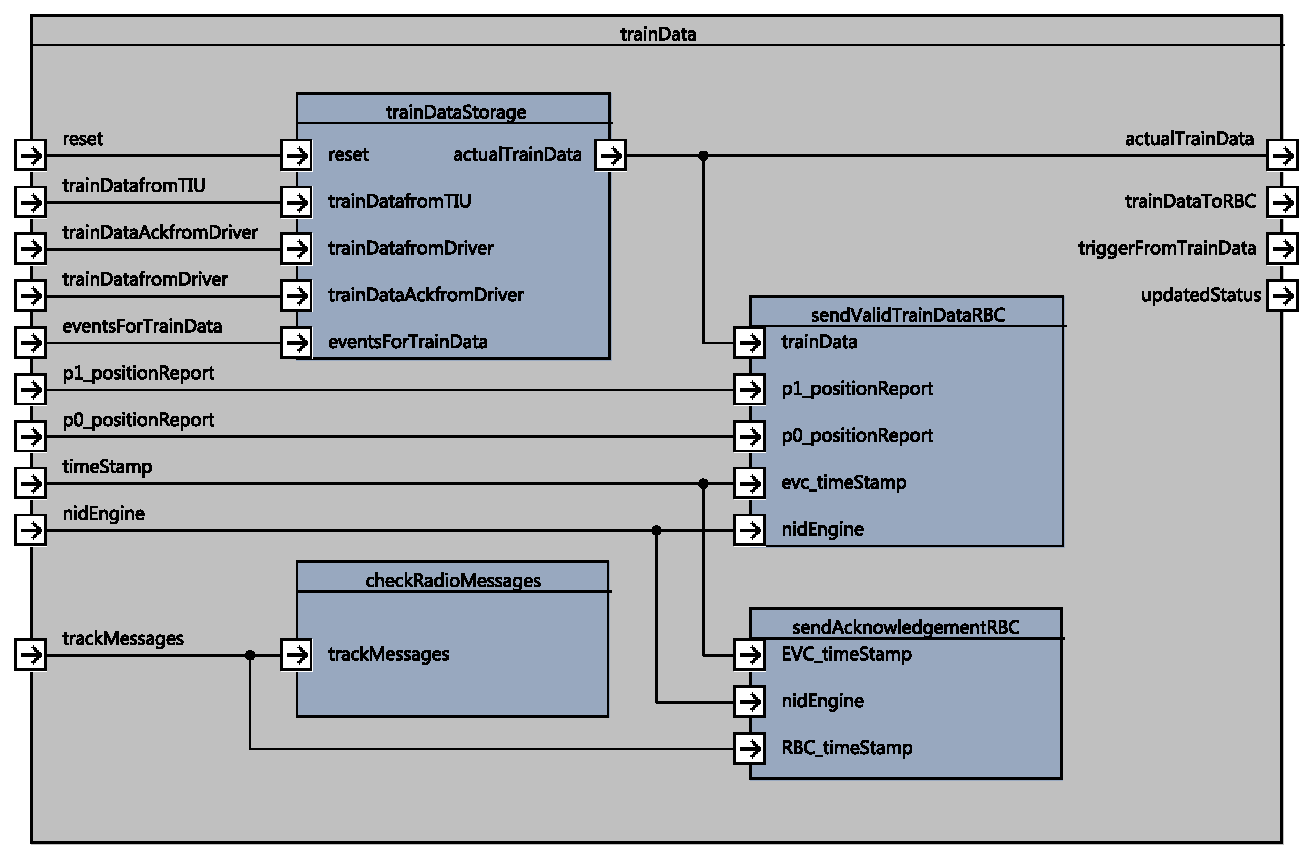
\includegraphics[width=\textwidth]{./images/F2_3_trainData_SysML.pdf}
\caption{trainData component SysML diagram.}\label{f:traindata_interface}
\end{figure}


\subsubsection{Inputs}\label{s:traindata_inputs}

\paragraph{reset}

\begin{longtable}{p{.25\textwidth}p{.7\textwidth}}
\toprule
Input name				& reset \\
\midrule
Description				& Triggers the reset of the train data and the train data status data.\\
\midrule
Source					& Persistent data status management.
\todo[inline]{Can't we reference a component of the model or input of F2 here?}\\ 
\midrule
Type					& bool \\
\midrule
Valid range of values	& 
\begin{description}
\item[true] Perform reset of train data and train data status.
\item[false] No reset of data in this cycle.
\end{description}
\\
\midrule
Behaviour when value is at boundary	& n/a \\
\midrule
Behaviour for values out of valid range	& n/a \\
\midrule
Behaviour when value is erroneous, absent or unwanted (i.e. spurious) & n/a \\
\bottomrule
\end{longtable}

\paragraph{trainDatafromTIU}

\begin{longtable}{p{.25\textwidth}p{.7\textwidth}}
\toprule
Input name				& trainDatafromTIU \\
\midrule
Description				& Train data received via TIU. The availability of data is indicated with the valid flag. This data is expected to be received in the first place. In the current implementation it is not supported to change data after a mission has been started.  The structure covers the following components:
\begin{description}
\item[valid](bool): valid indicator for this component. In this structure valid means the data has been received from train. Addition states like validated by driver or validated by RBC are maintained in the status structure for train data.
\item[other components]:  Other components are defined according to Section 3.18.3.2 of Subset-026. 
\end{description} \\
\midrule
Source					& Train Interface Unit (TIU)
\todo[inline]{Can't we reference a component of the model or input of F2 here?}\\ 
\midrule
Type					& TIU\_Types\_Pkg::trainData\_T \\
\midrule
Valid range of values	& Input with valid information is indicated with the valid flag set to true. 
\\
\midrule
Behaviour when value is at boundary	& n/a\\
\midrule
Behaviour for values out of valid range	& When valid flag indicates false the data to be used is assumed to be default values. The component is not used when valid flag is false.\\
\midrule
Behaviour when value is erroneous, absent or unwanted (i.e. spurious) & Information is only expected during the Start of Mission Procedure. Once the information is successfully received it is not considered any more. Change of train data by train during mission is not supported by this version of the openETCS OBU model.\\
\bottomrule
\end{longtable}

\paragraph{trainDatafromDriver}

\begin{longtable}{p{.25\textwidth}p{.7\textwidth}}
\toprule
Input name				& trainDatafromDriver \\
\midrule
Description				& Train data received via DMI from the driver. The availability of data is indicated with the valid flag. The data is expected as a mandatory parameter during start of mission. In the current implementation it is not supported to change data after a mission has been started. The structure consists of the following components:
\begin{description}
\item[valid](bool): valid indicator for this component. The data has been received from DMI. The flag is set to TRUE for a single cycle. 
\item[systemTime](Obu\_BasicTypes\_Pkg::T\_internal\_Type): timestamp set by the DMI. The component is not used by trainData.
\item[trainCtategory](NC\_TRAIN): Train category used for the static speed profile calculation.
Thanks to NC\_TRAIN, the train knows the SSP it must obey. Each bit represents one category. A train can belong to various categories.
\item[l\_train](Obu\_BasicTypes\_Pkg::L\_internal\_Type): Length of the train [cm].
\item[m\_brakeperct](int): brake percentage. range from 0 to 300.
\todo[inline]{If this is a percentage, then the range would probably be 0\ldots 100. Maybe we should replace percentage here?}
\item[v\_maxtrain](Obu\_BasicTypes\_Pkg::V\_internal\_Type): maximum speed of the train in km/h.
\todo[inline]{needs to be changed to cm/sec}
\item[m\_axleLoad](M\_AXLELOADCAT): axle load category according to Subset-026, Section 3.18.3.2.
\item[m\_airTight](M\_AIRTIGHT): airtight system presence according to Subset-026, Section 3.18.3.2.
\item[m\_loadingGauge](M\_LOADINGGAUGE): loading gauge category according to Subset-026, Section 3.18.3.2.
\end{description} \\

\midrule
Source				& Driver Machine Interface (DMI) 
\todo[inline]{Can't we reference a component of the model or input of F2 here?}\\ 
\midrule
Type					& DMI\_Messages\_Bothways\_Pkg::DMI\_Train\_Data\_T \\
\midrule
Valid range of values	& Input with valid information is indicated with the valid flag. \\
\midrule
Behaviour when value is at boundary	& n/a\\
\midrule
Behaviour for values out of valid range	& When valid flag indicates false the data to be used is assumed to be default values. The component is not used when valid flag is false.\\
\midrule
Behaviour when value is erroneous, absent or unwanted (i.e. spurious) & No checks on individual values is done in this part of the openETCS EVC. We assume - if necessary - appropriate checks are part of the interface layer (e.g., CRC checks) This type of checks is not in the scope of the openETCS project.\\
\bottomrule

\end{longtable}

\paragraph{trainDataAckfromDriver}

\begin{longtable}{p{.25\textwidth}p{.7\textwidth}}
\toprule
Input name				& trainDataAckfromDriver \\
\midrule
Description				& During start of mission the driver has to validate the train data. The confirmation is visible  based on this input. The structure looks like:
\begin{description}
\item[valid](bool): valid indicator for this component. The data has been received from DMI. The flag is set to TRUE for a single cycle. 
\item[systemTime](Obu\_BasicTypes\_Pkg::T\_internal\_Type): timestamp set by the DMI. The component is not used by trainData.
\item[acknowledged](bool): Result of the driver's acknoledgment.
\end{description} \\
\midrule
Source					& Driver Machine Interface (DMI) 
\todo[inline]{Can't we reference a component of the model or input of F2 here?}\\ 
\midrule
Type					& DMI\_Messages\_DMI\_to\_EVC\_Pkg::DMI\_Train\_Data\_Ack\_T \\
\midrule
Valid range of values	& Input with valid information is indicated with the valid flag. In addition, the ack parameter has to be evaluated in order to recognise the decision of the driver.\\
\midrule
Behaviour when value is at boundary	& n/a\\
\midrule
Behaviour for values out of valid range	& When valid flag is false the component will not be used and default values will be used instead.
\todo[inline]{This description was ambiguous. I tried to be more precise. Please check if this is still correct.}\\
\midrule
Behaviour when value is erroneous, absent or unwanted (i.e. spurious) & No checking on individual values is done in this part of the openETCS EVC. We assume - if necessary - appropriate checks are part of the interface layer (e.g., CRC checks) This type of checks is not in the scope of the openETCS project.\\

\bottomrule
\end{longtable}
\paragraph{trackMessages}

\begin{longtable}{p{.25\textwidth}p{.7\textwidth}}
\toprule
Input name				& trackMessages \\
\midrule
Description				& Information carries the message received from RBC. Information is only used when the valid flag is true and the message source is Radio. Other information is not relevant. Information is evaluated as long as the validation procedure is not completed and a valdiation request with the RBC is pending. \\
\midrule
Source					& Radio Transmission Module (RTM)
\todo[inline]{Can't we reference a component of the model or input of F2 here?}\\ 
\midrule
Type					& Common\_Types\_Pkg::ReceivedMessage\_T \\
\midrule
Valid range of values	& Input with valid information is indicated with the valid flag.\\
\midrule
Behaviour when value is at boundary	& n/a\\
\midrule
Behaviour for values out of valid range	& 
When valid flag indicates false the data to be used is assumed to be default values. The component is not used when valid flag is false.\\
\midrule
Behaviour when value is erroneous, absent or unwanted (i.e. spurious) & 
No checking on individual values is done in this part of the openETCS EVC. We assume - if necessary - appropriate checks are part of the interface layer (e.g., CRC checks) This type of checks is not in the scope of the openETCS project.\\

\bottomrule
\end{longtable}

\paragraph{timeStamp}

\begin{longtable}{p{.25\textwidth}p{.7\textwidth}}
\toprule
Input name				& timeStamp \\
\midrule
Description				& Timestamp for messaging to the RBC.\\
\midrule
Source					& Derived from train time.
\todo[inline]{Should we reference the corresponding input of F2 here?}\\ 
\midrule
Type						& T\_TRAIN\\
\midrule
Valid range of values			& Positive non-zero real\\
\midrule
Behaviour when value is at boundary	& Parameter is not used for computation or addressing. No impact in this model.\\
\midrule
Behaviour for values out of valid range	& No impact in the EVC. Communication to the RBC will be broken.\\
\midrule
Behaviour when value is erroneous, absent or unwanted (i.e. spurious) & Communication to the RBC will be broken. No safety issue in the EVC since RBC connection errors are covered by the EVC function.
\\
\bottomrule
\end{longtable}


\paragraph{eventsForTrainData}

\begin{longtable}{p{.25\textwidth}p{.7\textwidth}}
\toprule
Input name				& eventsForTrainData\\
\midrule
Description				& Timestamp for messaging to the RBC. Information of the EVC relevant for train data handling according to Section 3.18.3. In the current state of implementation the following events are evaluated:
\begin{itemize}
\item train stand-still
\item communication Session established
\end{itemize}
The MoRC ready input is used to indicate the evc:morc function is ready with acknowledgment of the communication session.\\
\midrule
Source					& EVC model.
\todo[inline]{Can't we reference a component of the model or input of F2 here?}\\ 
\midrule
Type						& trainData\_Types\_pkg::trainData\_Events\_T\\
\midrule
Valid range of values	& Structure of a set of bool. Each component may be true or false.\\
\midrule
Behaviour when value is at boundary	& n/a\\
\midrule
Behaviour for values out of valid range	& n/a\\
\midrule
Behaviour when value is erroneous, absent or unwanted (i.e. spurious) & n/a\\

\bottomrule
\end{longtable}

\paragraph{nidEngine}

\begin{longtable}{p{.25\textwidth}p{.7\textwidth}}
\toprule
Input name				& nidEngine\\
\midrule
Description				& ID of the engine. This ID is used in communication with the RBC in order to uniquely identify the engine.\\
\midrule
Source					& Configuration
\todo[inline]{Can't we reference a component of the model or input of F2 here?}\\ 
\\ 
\midrule
Type					& NID\_ENGINE\\
\midrule
Valid range of values	& Structure of a set of bool. Each component may be true or false.\\
\midrule
Behaviour when value is at boundary	& n/a\\
\midrule
Behaviour for values out of valid range	& n/a\\
\midrule
Behaviour when value is erroneous, absent or unwanted (i.e. spurious) & n/a\\

\bottomrule
\end{longtable}
\paragraph{p0\_positionReport}

\begin{longtable}{p{.25\textwidth}p{.7\textwidth}}
\toprule
Input name				& p0\_positionReport\\
\midrule
Description				& Actual Position Report (packet 0) for communication with the RBC.
\\
\midrule
Source					& EVC model.
\todo[inline]{Can't we reference a component of the model or input of F2 here?}\\ 
\midrule
Type					& Packet\_TrainTypes\_Pkg::PT0\_PositionReport\_T\\
\midrule
Valid range of values	& This packet is administered by a valid flag.\\
\midrule
Behaviour when value is at boundary	& n/a\\
\midrule
Behaviour for values out of valid range	& n/a\\
\midrule
Behaviour when value is erroneous, absent or unwanted (i.e. spurious) & n/a\\
\bottomrule
\end{longtable}

\paragraph{p1\_positionReport}

\begin{longtable}{p{.25\textwidth}p{.7\textwidth}}
\toprule
Input name				& p1\_positionReport\\
\midrule
Description				& Actual Position Report (packet 1) for communication with the RBC.
\\
\midrule
Source					& EVC model.
\todo[inline]{Can't we reference a component of the model or input of F2 here?}\\  
\midrule
Type						& Packet\_TrainTypes\_Pkg::PT1\_PositionReport\_2BG\_T\\
\midrule
Valid range of values	& This packet is administered by a valid flag.\\
\midrule
Behaviour when value is at boundary	& n/a\\
\midrule
Behaviour for values out of valid range	& n/a\\
\midrule
Behaviour when value is erroneous, absent or unwanted (i.e. spurious) & n/a\\
\bottomrule
\end{longtable}

\subsubsection{Outputs}\label{s:traindata_outputs}

\paragraph{actualTrainData}

\begin{longtable}{p{.25\textwidth}p{.7\textwidth}}
\toprule
Output name				& actualTrainData \\
\midrule
Description				& Actual train data of the evc. Train data received via DMI from the driver. The availability of data is indicated with the valid flag. The data is expected as a mandatory parameter during start of mission. In the current implementation it is not supported to change data after a mission has been started. The structure consists of the following components:
\begin{description}
\item[valid](bool): valid indicator for this component. Valid indicates the data are updated after start-up of the system. The actual status of trainData is stored in the updatedStatus information. 
\item[acknowledgedByDriver](bool): Indicates this component has been validated by the driver.
\todo[inline]{redundant information to status. Needs cleaning}
\item[trainCtategory](NC\_TRAIN): Train category used for the static speed profile calculation.
\item[cantDeficientcy](NC\_CDTRAIN): Cant deficiency train category
\item[trainLength](Obu\_BasicTypes\_Pkg::L\_internal\_Type): Length of the train [cm].
\item[brakePercentage](int): brake percentage. range from 0 to 300.
\item[maxTrainSpeed](Obu\_BasicTypes\_Pkg::V\_internal\_Type): maximum speed of the train in km/h.
\todo[inline]{needs to be changed to cm/sec}
\item[loadingGauge](M\_LOADINGGAUGE): loading gauge category according to 3.18.3.2
\item[axleLoadCategory](M\_AXLELOADCAT): axle load category according to Subset-026, Section 3.18.3.2.
\item[airTightSystem](M\_AIRTIGHT): airtight system presence according to Subset-026, Section 3.18.3.2.
\item[axleNumber]int): axle number according to Subset-026, Section 3.18.3.2.
\item[numberNationalSystems](int): The number of national systems available in the train.
\item[nationalSystems](Packet\_TrainTypes\_Pkg::aNID\_NTC\_T): National Systems available in the train. The elements 0 .. numberNationalSystems - 1 are carrying the relevant data.
\item[numberTractionSystems](int): The number of traction systems available in the train.
\item[tractionSystems](Packet\_TrainTypes\_Pkg::aTractionIdentity\_T): Traction Systems available in the train. The elements 0 \ldots numberTractionSystems - 1 are carrying the relevant data.
\end{description} \\


\midrule
Destination				& ???  
\todo[inline]{we have to reference a component of the model or input of F2 here}\\ 
\\ 
\midrule
Type						& TIU\_Types\_Pkg::trainData\_T \\
\midrule
Valid range of values			& n/a \\
\midrule
Behaviour when value is at boundary	& n/a \\
\midrule
Behaviour for values out of valid range	& n/a \\
\midrule
Behaviour when value is erroneous, absent or unwanted (i.e. spurious) &n/a \\
\bottomrule
\end{longtable}

\paragraph{trainDataToRBC}

\begin{longtable}{p{.25\textwidth}p{.7\textwidth}}
\toprule
Output name				& trainDataToRBC \\
\midrule
Description				& Messages for communicating with the RBC. Messages 129 (Validated Train Data) and 146 (Acknowledgement) are sent by this function. The presence of the message is indicated by a valid flag.\\
\midrule
Destination				& Radio Output 
\todo[inline]{Can't we reference a component of the model or input of F2 here?}\\ 
\\ 
\midrule
Type					& Radio\_Types\_Pkg::Radio\_TrainTrack\_Message\_T \\
\midrule
Valid range of values	& indicated by valid flag. \\
\midrule
Behaviour when value is at boundary	& n/a\\
\midrule
Behaviour for values out of valid range	& n/a \\
\midrule
Behaviour when value is erroneous, absent or unwanted (i.e. spurious) & n/a\\
\bottomrule
\end{longtable}

\paragraph{triggerFromTrainData}

\begin{longtable}{p{.25\textwidth}p{.7\textwidth}}
\toprule
Output name				& triggerFromTrainData \\
\midrule
Description				& For a full implementation of ETCS trainDAta has additional tasks described in the standard but not implemented in openETCS. For those extensions the triggers are pre-defined. \\
\midrule
Destination				& evc \\ 
\midrule
Type					& trainData\_Types\_pkg::trainData\_Trigger\_T
 \\
\midrule
Valid range of values	& n/a \\
\midrule
Behaviour when value is at boundary	& n/a\\
\midrule
Behaviour for values out of valid range	& n/a \\
\midrule
Behaviour when value is erroneous, absent or unwanted (i.e. spurious) & n/a\\
\bottomrule
\end{longtable}

\paragraph{updatedStatus}

\begin{longtable}{p{.25\textwidth}p{.7\textwidth}}
\toprule
Output name				& updatedStatus \\
\midrule
Description				& Detailed definition of the trainData status. The following components are defined:
\begin{description}
\item[valid](bool): Data is initialised based on data received from the TIU.
\item[validatedByDriver](bool): Data has been validated by the Driver.
\item[validatedbyRBC](bool): Data has been validated by the RBC.
\item[waitingForRBCResponse](bool): 3.18.3.4.1 Train is waiting for ack to validation command.
\item[driverIsModificationTrainData](bool):3.18.3.3.1 Driver is Modifying / Revalidating train data.
\item[timeStampValidateToRBC](T\_TRAIN): 8.7.4 This label is used in communication with the RBC to identify the communication entity. Train data is acknowledged.
\end{description} 
\\
\midrule
Destination				& evc
\todo[inline]{Can't we reference a component of the model or input of F2 here?}\\  
\midrule
Type					& trainData\_Types\_pkg::trainDataStatus\_T \\
\midrule
Valid range of values	& indicated by valid flag. \\
\midrule
Behaviour when value is at boundary	& n/a\\
\midrule
Behaviour for values out of valid range	& n/a \\
\midrule
Behaviour when value is erroneous, absent or unwanted (i.e. spurious) & n/a\\
\bottomrule
\end{longtable}

\subsection{Subcomponents}\label{s:traindata_subcomponents}

\todo[inline]{section needs to be completed}

\subsubsection{trainDataStorage}
%set the master document for easy compilation
%!TEX root = ../D3_5_3.tex

\paragraph{Component Requirements}

\begin{longtable}{p{.25\textwidth}p{.7\textwidth}}
\toprule
Component name			& trainDataStorage \\
\midrule
Link to SCADE model		& {\footnotesize {\url{https://github.com/openETCS/modeling/blob/master/model/Scade/System/ObuFunctions/manageData/trainData/trainData.etp}}} \\
\midrule
SCADE designer			& Bernd Hekele, DB Netz AG \\
\midrule
Description				& Storage of trainData information. The format of the data kept is described above. Data can be stored or merged depending on the source of data. A reset function is forseen for initialisation of data. \\
\midrule
Input documents	& 
Subset-026, Chapter 3.18.3\\
\midrule
Safety integrity level	& 4 \\
\midrule
Time constraints		& n/a \\
\midrule
API requirements 		& n/a \\
\bottomrule
\end{longtable}


\paragraph{Interface}

For an overview of the interface of this internal component we refer to the SCADE model (cf.~link above) respectively the SCADE generated documentation.

\subsubsection{checkRadioMessages}
%set the master document for easy compilation
%!TEX root = ../D3_5_3.tex

\paragraph{Component Requirements}

\begin{longtable}{p{.25\textwidth}p{.7\textwidth}}
\toprule
Component name			& checkRadioMessages \\
\midrule
Link to SCADE model		& {\footnotesize {\url{https://github.com/openETCS/modeling/blob/master/model/Scade/System/ObuFunctions/manageData/trainData/trainData.etp}}} \\
\midrule
SCADE designer			& Bernd Hekele, DB Netz AG \\
\midrule
Description				& The function checks an incoming radio message for relevance in the trainData context. Result is whether the message requests an acknowledgement and whether the radio message is a response to an outstanding validation request.\\
\midrule
Input documents	& 
Subset-026, Chapter 3.18.3\\
\midrule
Safety integrity level	& 4 \\
\midrule
Time constraints		& n/a \\
\midrule
API requirements 		& n/a \\
\bottomrule
\end{longtable}


\paragraph{Interface}

For an overview of the interface of this internal component we refer to the SCADE model (cf.~link above) respectively the SCADE generated documentation.

\subsubsection{sendValidTrainDataRBC}
%set the master document for easy compilation
%!TEX root = ../D3_5_3.tex

\paragraph{Component Requirements}

\begin{longtable}{p{.25\textwidth}p{.7\textwidth}}
\toprule
Component name			& sendValidTrainDataRBC \\
\midrule
Link to SCADE model		& {\footnotesize {\url{https://github.com/openETCS/modeling/blob/master/model/Scade/System/ObuFunctions/manageData/trainData/trainData.etp}}} \\
\midrule
SCADE designer			& Bernd Hekele, DB Netz AG \\
\midrule
Description				& This function send the validate data request ot the RBC an updates trainData States with the relevant information.\\
\midrule
Input documents	& 
Subset-026, Chapter 3.18.3\\
\midrule
Safety integrity level	& 4 \\
\midrule
Time constraints		& n/a \\
\midrule
API requirements 		& n/a \\
\bottomrule
\end{longtable}


\paragraph{Interface}

For an overview of the interface of this internal component we refer to the SCADE model (cf.~link above) respectively the SCADE generated documentation.

\subsubsection{sendAcknowledgementRBC}
%set the master document for easy compilation
%!TEX root = ../D3_5_3.tex

\paragraph{Component Requirements}

\begin{longtable}{p{.25\textwidth}p{.7\textwidth}}
\toprule
Component name			& sendAcknowledgementRBC \\
\midrule
Link to SCADE model		& {\footnotesize {\url{https://github.com/openETCS/modeling/blob/master/model/Scade/System/ObuFunctions/manageData/trainData/trainData.etp}}} \\
\midrule
SCADE designer			& Bernd Hekele, DB Netz AG \\
\midrule
Description				& This function prepares the Information foracknowledgement message. It is assumed it used with an boolean activator. \\
\midrule
Input documents	& 
Subset-026, Chapter 3.18.3\\
\midrule
Safety integrity level	& 4 \\
\midrule
Time constraints		& n/a \\
\midrule
API requirements 		& n/a \\
\bottomrule
\end{longtable}


\paragraph{Interface}

For an overview of the interface of this internal component we refer to the SCADE model (cf.~link above) respectively the SCADE generated documentation.

\subsubsection{checkAcknowledgementGeneral}
%set the master document for easy compilation
%!TEX root = ../D3_5_3.tex

\paragraph{Component Requirements}

\begin{longtable}{p{.25\textwidth}p{.7\textwidth}}
\toprule
Component name			& checkAcknowledgementGeneral \\
\midrule
Link to SCADE model		& {\footnotesize {\url{https://github.com/openETCS/modeling/blob/master/model/Scade/System/ObuFunctions/manageData/trainData/trainData.etp}}} \\
\midrule
SCADE designer			& Bernd Hekele, DB Netz AG \\
\midrule
Description				& This function implements the acknowledment to ma request and general message. It is actually an extension of the trainData function and needs to be moved to radio management functions.\\
\midrule
Input documents	& 
Subset-026, Chapter 3.18.3\\
\midrule
Safety integrity level	& 4 \\
\midrule
Time constraints		& n/a \\
\midrule
API requirements 		& n/a \\
\bottomrule
\end{longtable}


\paragraph{Interface}

For an overview of the interface of this internal component we refer to the SCADE model (cf.~link above) respectively the SCADE generated documentation.





%set the master document for easy compilation
%!TEX root = ../D3_5_3.tex

\section{F2.4: TrackAtlas}\label{s:F2.4}
\todo[inline]{Section needs to be completed}

\subsection{Component Requirements}

\begin{longtable}{p{.25\textwidth}p{.7\textwidth}}
\toprule
Component name			& TrackAtlas \\
\midrule
Link to SCADE model		& {\footnotesize \url{???}} \\
\midrule
SCADE designer			& Jakob G\"artner, LEA \\
\midrule
Description				& ??? \\
\midrule
Input documents	& 
Subset-026, Chapter ???\\
\midrule
Safety integrity level	& 4 \\
\midrule
Time constraints		& [If applicable description of time constraints, otherwise n/a] \\
\midrule
API requirements 		& [If applicable description of API requirements, otherwise n/a] \\
\bottomrule
\end{longtable}


\subsection{Interface}

An overview of the interface of component TrackAtlas is shown in Figure~\ref{f:manage_track_data_interface}. The inputs and outputs are described in detail in Section~\ref{s:manage_track_data_inputs} respectively \ref{s:manage_track_data_outputs}. Subcomponents are described in Section~\ref{s:manage_track_data_subcomponents}.

\begin{figure}
\center
\missingfigure{[Put SysML diagram of component here]}
\caption{TrackAtlas component SysML diagram}\label{f:manage_track_data_interface}
\end{figure}


\subsubsection{Inputs}\label{s:manage_track_data_inputs}

\paragraph{[Input 1 name]}

\begin{longtable}{p{.25\textwidth}p{.7\textwidth}}
\toprule
Input name				& [Name of the input] \\
\midrule
Description				& [Brief description of the input] \\
\midrule
Source					& [Name of the source component] \\ 
\midrule
Type					& [Type of the input] \\
\midrule
Valid range of values	& [Complete list of valid values] \\
\midrule
Behaviour when value is at boundary	& [Description of components behaviour when input value is at boundary] \\
\midrule
Behaviour for values out of valid range	& [Description of components behaviour when input value is out of valid range] \\
\midrule
Behaviour when value is erroneous, absent or unwanted (i.e. spurious) & [Description of components behaviour when value is erroneous, absent or unwanted (i.e. spurious)] \\
\bottomrule
\end{longtable}


\paragraph{[Input 2 name]}

\begin{longtable}{p{.25\textwidth}p{.7\textwidth}}
\toprule
Input name				& [Name of the input] \\
\midrule
Description				& [Brief description of the input] \\
\midrule
Source					& [Name of the source component] \\ 
\midrule
Type					& [Type of the input] \\
\midrule
Valid range of values	& [Complete list of valid values] \\
\midrule
Behaviour when value is at boundary	& [Description of components behaviour when input value is at boundary] \\
\midrule
Behaviour for values out of valid range	& [Description of components behaviour when input value is out of valid range] \\
\midrule
Behaviour when value is erroneous, absent or unwanted (i.e. spurious) & [Description of components behaviour when value is erroneous, absent or unwanted (i.e. spurious)] \\
\bottomrule
\end{longtable}


\subsubsection{Outputs}\label{s:manage_track_data_outputs}

\paragraph{[Output 1 name]}

\begin{longtable}{p{.25\textwidth}p{.7\textwidth}}
\toprule
Output name				& [Name of the output] \\
\midrule
Description				& [Brief description of the output] \\
\midrule
Destination				& [Name of the destination component(s)] \\ 
\midrule
Type					& [Type of the output] \\
\midrule
Valid range of values	& [Complete list of valid values] \\
\midrule
Behaviour when value is at boundary	& [Description of components behaviour when output value is at boundary] \\
\midrule
Behaviour for values out of valid range	& [Description of components behaviour when output value is out of valid range] \\
\midrule
Behaviour when value is erroneous, absent or unwanted (i.e. spurious) & [Description of components behaviour when value is erroneous, absent or unwanted (i.e. spurious)] \\
\bottomrule
\end{longtable}


\paragraph{[Output 2 name]}

\begin{longtable}{p{.25\textwidth}p{.7\textwidth}}
\toprule
Output name				& [Name of the output] \\
\midrule
Description				& [Brief description of the output] \\
\midrule
Destination				& [Name of the destination component(s)] \\ 
\midrule
Type					& [Type of the output] \\
\midrule
Valid range of values	& [Complete list of valid values] \\
\midrule
Behaviour when value is at boundary	& [Description of components behaviour when output value is at boundary] \\
\midrule
Behaviour for values out of valid range	& [Description of components behaviour when output value is out of valid range] \\
\midrule
Behaviour when value is erroneous, absent or unwanted (i.e. spurious) & [Description of components behaviour when value is erroneous, absent or unwanted (i.e. spurious)] \\
\bottomrule
\end{longtable}


\subsection{Subcomponents}\label{s:manage_track_data_subcomponents}

\subsubsection{StoreRaw\_NV}
\input{sections/StoreRaw_NV.tex}

\subsubsection{Build\_GradientProfile}
\input{sections/Build_GradientProfile.tex}

\subsubsection{Build\_MA}
\input{sections/Build_MA.tex}

\subsubsection{Build\_MRSP}
\input{sections/Build_MRSP.tex}

\subsubsection{Manage\_EmergencyStop}
\input{sections/Manage_EmergencyStop.tex}

\subsubsection{C\_P003V1\_OBU\_P003\_OBU}
\input{sections/C_P003V1_OBU_P003_OBU.tex}

\subsubsection{GradientProfile\_to\_DMI}
\input{sections/GradientProfile_to_DMI.tex}

\subsubsection{Manage\_MA\_Request}
\input{sections/Manage_MA_Request.tex}

\subsubsection{TA\_to\_ML}
\input{sections/TA_to_ML.tex}

\subsubsection{SSP\_to\_MRSP}
\input{sections/SSP_to_MRSP.tex}

\subsubsection{MRSP\_to\_MRSP\_to\_DMI}
\input{sections/MRSP_to_MRSP_to_DMI.tex}



%set the master document for easy compilation
%!TEX root = ../D3_5_3.tex

\section{F2.5: ManageLevelAndMode}\label{s:F2.5}

\subsection{Component Requirements}

\begin{longtable}{p{.25\textwidth}p{.7\textwidth}}
\toprule
Component name			& ManageLevelAndMode \\
\midrule
Link to SCADE model		& {\footnotesize \url{https://github.com/openETCS/modeling/tree/master/model/Scade/System/ObuFunctions/ManageLevelsAndModes}} \\
\midrule
SCADE designer			& Marielle Petit-Doche and  Matthias G\"udemann, Systerel \\
\midrule
Description				& Modes and levels define the status of the ETCS
regarding on-board functional status and track infrastructure. \\
\midrule
Input documents	& 
Subset-026, Chapter 4 \newline
Subset-026, Chapter 5 \\
\midrule
Safety integrity level	& 4 \\
\midrule
Time constraints		&  n/a \\
\midrule
API requirements 		&  n/a \\
\bottomrule
\end{longtable}


\subsection{Interface}

An overview of the interface of component ManageLevelAndMode is shown in Figure~\ref{f:mode_and_level} and Figure~\ref{f:mode_and_level_interface}. The inputs and outputs are described in detail in Section~\ref{s:mode_and_level_inputs} respectively \ref{s:mode_and_level_outputs}. Subcomponents are described in Section~\ref{s:mdoe_and_level_subcomponents}.

\begin{figure}
\center
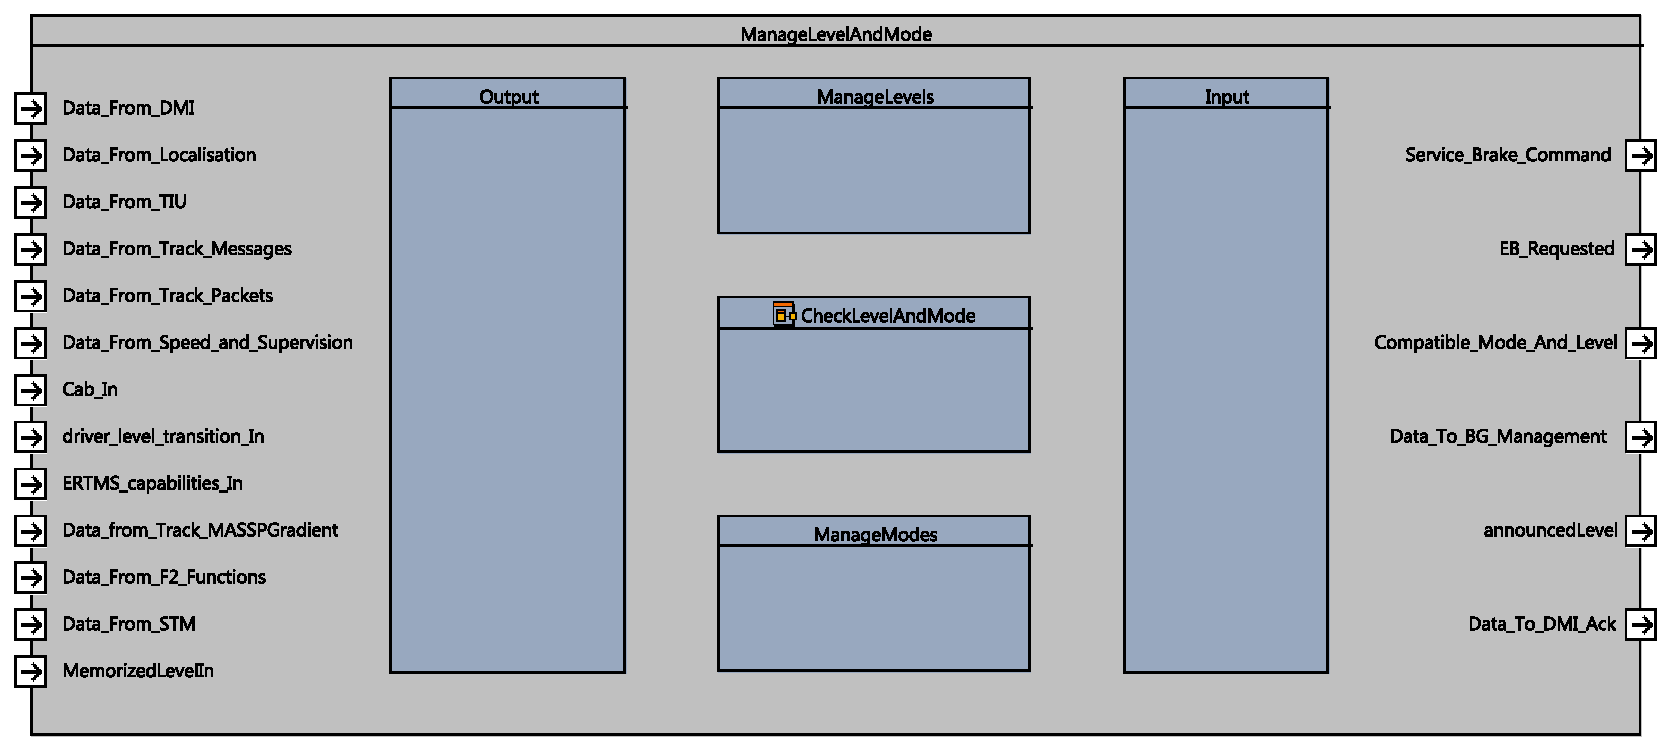
\includegraphics[width=\textwidth]{images/F2_5_ManageLevelsAndModes.pdf}
\caption{ManageLevelAndMode component SysML diagram.}\label{f:mode_and_level}
\end{figure}

\begin{figure}[p]
\center
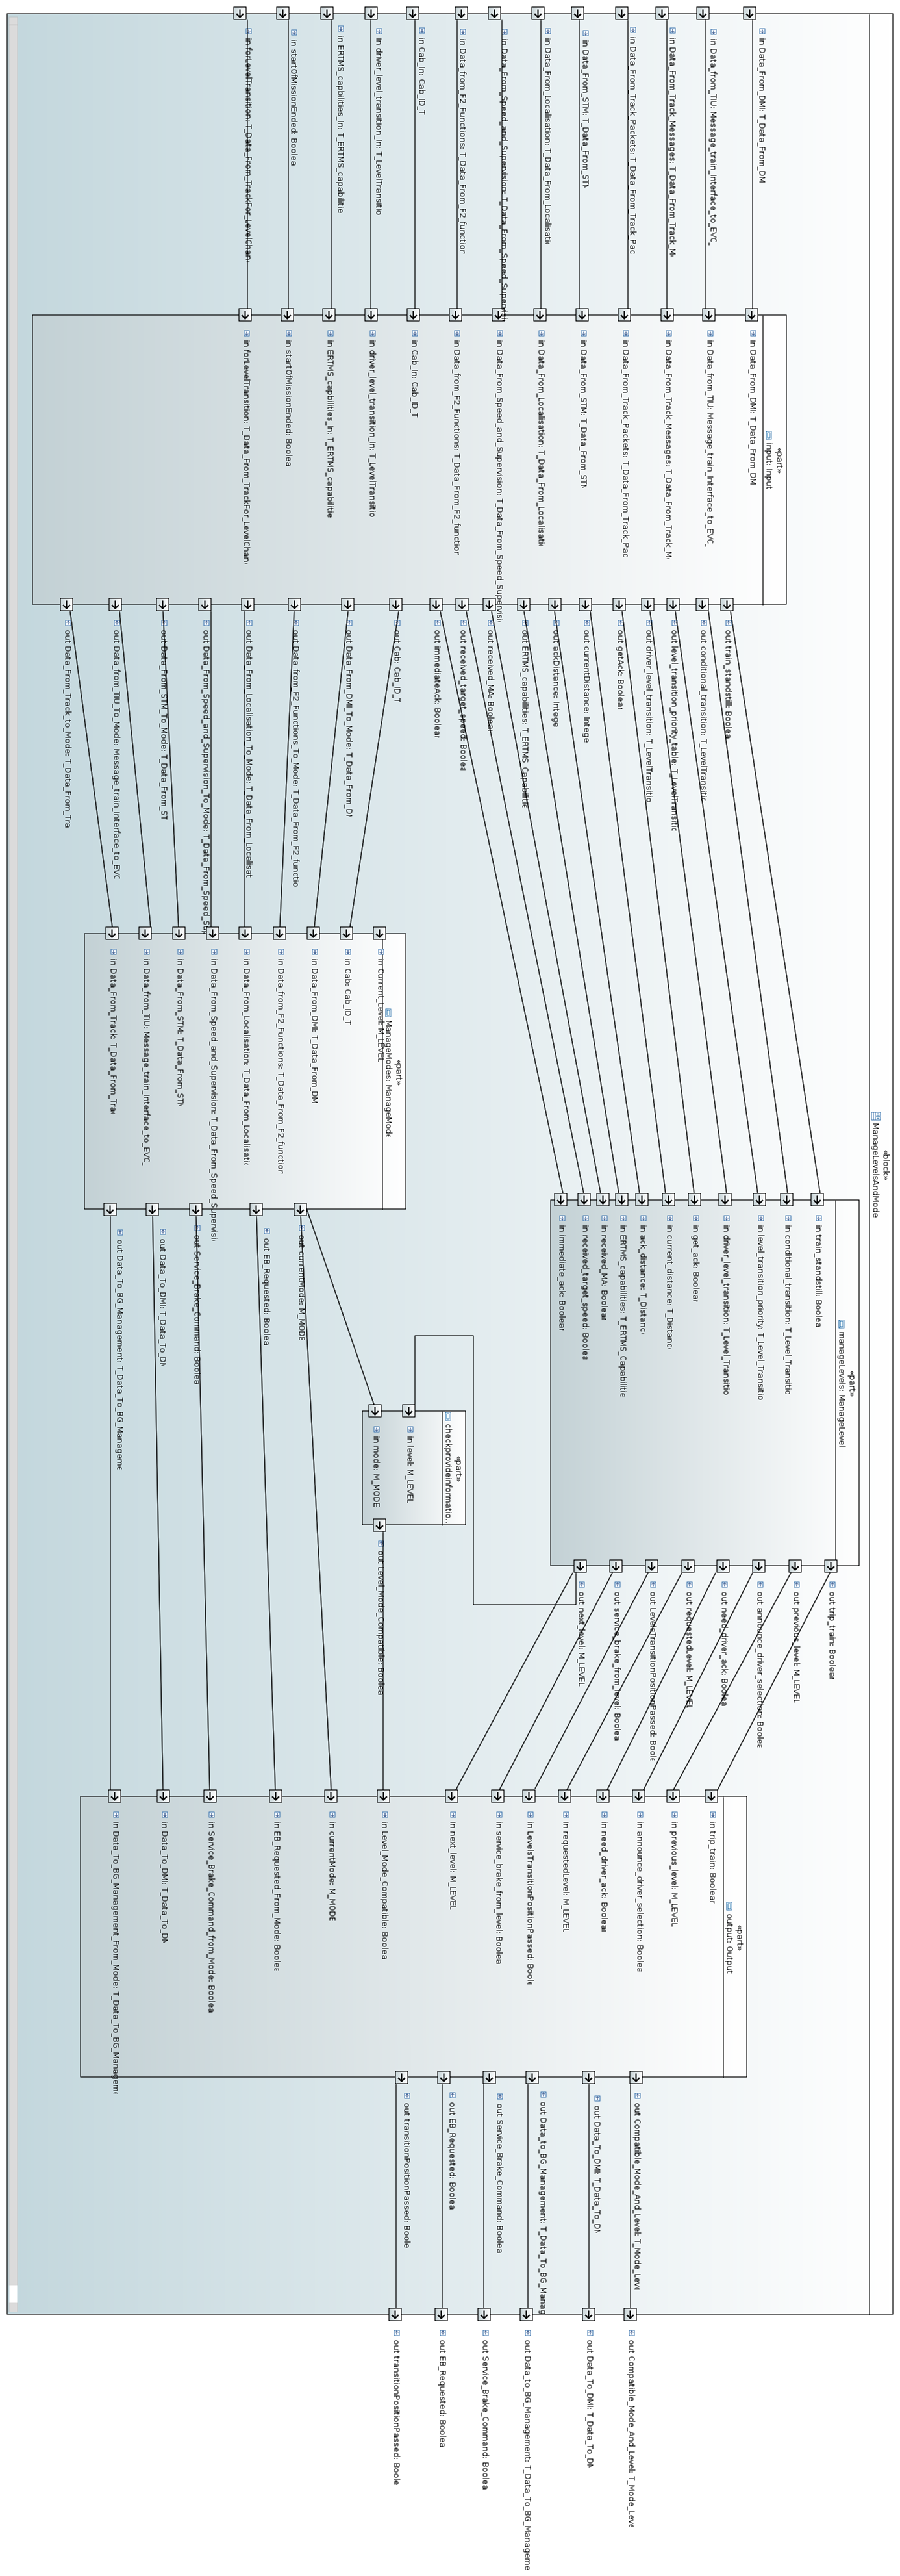
\includegraphics[height=\textheight]{images/ManageLevelsAndModes.png}
\caption{Mode\_and\_Level data flow SysML diagram}\label{f:mode_and_level_interface}
\end{figure}

For a detail description of the interface and contents of the Scade model see \url{https://github.com/openETCS/modeling/blob/master/model/Scade/System/ObuFunctions/ManageLevelsAndModes/ModesAndLevels/ModesAndLevels.pdf}, for types definition see : \url{https://github.com/openETCS/modeling/blob/master/model/Scade/System/ObuFunctions/ManageLevelsAndModes/Level_And_Mode_Types/Level_And_Mode_Types.pdf}

\subsubsection{Inputs}\label{s:mode_and_level_inputs}

See Figure~\ref{f:mode_and_level_inputs} for the inputs of the function.

\begin{figure}
\center
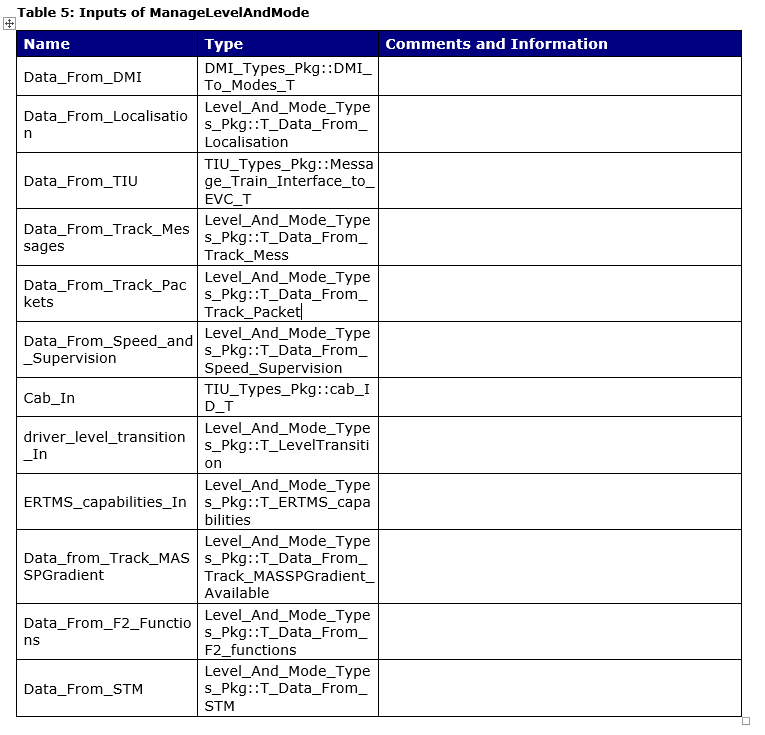
\includegraphics[width=\textwidth]{images/Inputs_ML.png}
\caption{Mode\_and\_Level inputs}\label{f:mode_and_level_inputs}
\end{figure}

\paragraph{Data\_From\_DMI}

\begin{longtable}{p{.25\textwidth}p{.7\textwidth}}
\toprule
Input name				& Data\_From\_DMI \\
\midrule
Description				& Set of data transmitted from DMI  (driver acknowledgements and requests to  switch modes and level) \\
\midrule
Source					& F2.10 manageDMI\_Input \\ 
\midrule
Type					& DMI\_Types\_Pkg::DMI\_To\_Modes\_T \\
\midrule
Valid range of values	& It is a complex type : 
\begin{itemize}
\item valid :  bool,  flag to inform of the freshness of the information
\item DriverAck : DMI\_DriverAck\_T, indicate which mode is acknoledged
\item DriverRequest : DMI\_DriverRequest\_T, table of boolean values for all the driver request related to  mode changes.
\item LevelAck : bool, indication of Level  change acknowledgement
\end{itemize} \\
\midrule
Behaviour when value is at boundary	& n/a \\ 
\midrule
Behaviour for values out of valid range	& n/a \\ 
\midrule
Behaviour when value is erroneous, absent or unwanted (i.e. spurious) & n/a \\ 
\bottomrule
\end{longtable}

\paragraph{Data\_From\_Localisation}

\begin{longtable}{p{.25\textwidth}p{.7\textwidth}}
\toprule
Input name				& Data\_From\_Localisation \\
\midrule
Description				& Set of data on position and speed of the train \\
\midrule
Source					& F2.6 calculateTrainPosition\newline
F2 input API\_Odometry \\ 
\midrule
Type					& Level\_And\_Mode\_Types\_Pkg::T\_Data\_From\_Localisation \\
\midrule
Valid range of values	& It is a complex type: 
\begin{itemize}
\item BG\_In\_List\_Expected\_BG\_In\_SR : bool,
\item  BG\_In\_List\_Expected\_BG\_In\_SH : bool, 
\item PositionErrors : TrainPosition\_Types\_Pck::positionErrors\_T,
\item  Train\_Position : TrainPosition\_Types\_Pck::trainPosition\_T,
\item Train\_Speed : Obu\_BasicTypes\_Pkg::Speed\_T, 
\item Train\_Standstill : bool
\end{itemize} \\
\midrule
Behaviour when value is at boundary	& n/a \\ 
\midrule
Behaviour for values out of valid range	& n/a \\ 
\midrule
Behaviour when value is erroneous, absent or unwanted (i.e. spurious) & n/a \\ 
\bottomrule
\end{longtable}

\paragraph{Data\_From\_TIU}

\begin{longtable}{p{.25\textwidth}p{.7\textwidth}}
\toprule
Input name				& Data\_From\_TIU \\
\midrule
Description				& Set of data providing by TIU \\
\midrule
Source					& F2.12 manageTIU\_input \\ 
\midrule
Type					& TIU\_Types\_Pkg::Message\_Train\_Interface\_to\_EVC\_T \\
\midrule
Valid range of values	& It is a complex type defined in the TIU package. \\
\midrule
Behaviour when value is at boundary	& n/a \\ 
\midrule
Behaviour for values out of valid range	& n/a \\ 
\midrule
Behaviour when value is erroneous, absent or unwanted (i.e. spurious) & n/a \\ 
\bottomrule
\end{longtable}


\paragraph{Data\_From\_Track\_Messages}

\begin{longtable}{p{.25\textwidth}p{.7\textwidth}}
\toprule
Input name				& Data\_From\_Track\_Messages \\
\midrule
Description				& Messages received from trackside contaigning information for modes and levels switches \\
\midrule
Source					& F2.4 TrackAtlas \\ 
\midrule
Type					& Level\_And\_Mode\_Types\_Pkg::T\_Data\_From\_Track\_Messages \\
\midrule
Valid range of values	& It is a complex type containing the information of messages : 2, 6, 15, 16, 27 and 28 \\
\midrule
Behaviour when value is at boundary	& n/a \\ 
\midrule
Behaviour for values out of valid range	& n/a \\ 
\midrule
Behaviour when value is erroneous, absent or unwanted (i.e. spurious) & n/a \\ 
\bottomrule
\end{longtable}


\paragraph{Data\_From\_Track\_Packets}

\begin{longtable}{p{.25\textwidth}p{.7\textwidth}}
\toprule
Input name				& Data\_From\_Track\_Packets \\
\midrule
Description				& Packets received from trackside contaigning information for modes and levels switches. \\
\midrule
Source					& F2.1 Manage\_TrackSideInformation\_Integration\\ 
\midrule
Type					& Level\_And\_Mode\_Types\_Pkg::T\_Data\_From\_Track\_Packet \\
\midrule
Valid range of values	& It is a complex type containing the information of packets : 12, 15, 21, 27, 41, 46, 63, 80, 135, 137, 138, and 139. \\
\midrule
Behaviour when value is at boundary	& n/a \\ 
\midrule
Behaviour for values out of valid range	& n/a \\ 
\midrule
Behaviour when value is erroneous, absent or unwanted (i.e. spurious) & n/a \\ 
\bottomrule
\end{longtable}




\paragraph{Data\_From\_speed\_and\_Supervision}


\begin{longtable}{p{.25\textwidth}p{.7\textwidth}}
\toprule
Input name				& Data\_From\_speed\_and\_Supervision \\
\midrule
Description				& Data provided by the speed and supervision function \\
\midrule
Source					& F2.7 SpeedSupervision\_Integraton \\ 
\midrule
Type					& Level\_And\_Mode\_Types\_Pkg::T\_Data\_From\_Speed\_Supervision \\
\midrule
Valid range of values	& Input type is a complex type:
\begin{itemize}
\item \emph{Estim\_front\_End\_overpass\_SR\_Dist : bool}: the train overpass the SR distance with its estimated front end (from SR to trip mode condition 42) 
\item \emph{Estim\_Front\_End\_Rear\_SSP : bool}: estimated front end is rear of the start location of either SSP or gradient profile stored on-board (from FS, LS, OS to trip mode condition 69)
\item \emph{Override\_Function\_Active}: boolean to indicate the state of the activation function 	  	
\item \emph{EOA\_Antenna\_Overpass : bool}: the train overpasses the  EOA  with min safe antenna position Level 1 (from FS, LS, OS to trip mode condition 12)
\item \emph{EOA\_Front\_End : bool} the train overpasses the  EOA  with min safe front end, Level 2 or 3 (from FS, LS, OS to trip mode condition 16)
\item \emph{Train\_Speed\_Under\_Overide\_Limit : bool} supervision when override function is active (to SR mode condition 37)
\end{itemize}\\
\midrule
Behaviour when value is at boundary	& n/a \\ 
\midrule
Behaviour for values out of valid range	& n/a \\ 
\midrule
Behaviour when value is erroneous, absent or unwanted (i.e. spurious) & n/a \\ 
\bottomrule
\end{longtable}



\paragraph{driver\_level\_transition\_in}

\begin{longtable}{p{.25\textwidth}p{.7\textwidth}}
\toprule
Input name				& driver\_level\_transition\_in \\
\midrule
Description				& Request of level transition given by the driver for example at start of mission \\
\midrule
Source					& F2.10 manageDMI\_Input \\ 
\midrule
Type					& Level\_And\_Modes\_Types\_Pkg::T\_LevelTransition \\
\midrule
Valid range of values	& It is a complex type:  
\begin{itemize}
\item is\_set : bool,
\item transition : Level\_And\_Mode\_Types\_Pkg::T\_LevelTansitionInfo, 
\item LRBG : NID\_LRBG, 
\item referenceLocation : Obu\_BasicTypes\_Pkg::L\_internal\_Type
\end{itemize} \\
\midrule
Behaviour when value is at boundary	& n/a \\ 
\midrule
Behaviour for values out of valid range	& n/a \\ 
\midrule
Behaviour when value is erroneous, absent or unwanted (i.e. spurious) & n/a \\ 
\bottomrule \\ 
\end{longtable}


\paragraph{Cab\_In}

\begin{longtable}{p{.25\textwidth}p{.7\textwidth}}
\toprule
Input name				& Cab\_In \\
\midrule
Description				& Identification of the cabine where the EVC is implemented. \\
\midrule
Source					& F2.12 manageTIU\_input \\ 
\midrule
Type					& TIU\_Types\_Pkg::cab\_ID\_T \\
\midrule
Valid range of values	&  [CabUndefined, CabA, CabB] \\
\midrule
Behaviour when value is at boundary	& n/a \\ 
\midrule
Behaviour for values out of valid range	& n/a \\ 
\midrule
Behaviour when value is erroneous, absent or unwanted (i.e. spurious) & n/a \\ 
\bottomrule
\end{longtable}


\paragraph{ERTMS\_Capabilities}

\begin{longtable}{p{.25\textwidth}p{.7\textwidth}}
\toprule
Input name				& ERTMS\_Capabilities \\
\midrule
Description				& Identification of the capabilities of the train in regards of ERTMS levels\\
\midrule
Source					& F2 input API\_persistentData \\ 
\midrule
Type					& T\_ERTMS\_Capabilities \\
\midrule
Valid range of values	& It is a complex type: 
\begin{itemize}
\item NTC : bool,
\item L0 : bool, 
\item L1 : bool, 
\item L2 : bool,
\item L3 : bool
\end{itemize} \\
\midrule
Behaviour when value is at boundary	& n/a \\ 
\midrule
Behaviour for values out of valid range	& n/a \\ 
\midrule
Behaviour when value is erroneous, absent or unwanted (i.e. spurious) & n/a \\ 
\bottomrule
\end{longtable}




\paragraph{Data\_From\_Track\_MASSPGradient}

\begin{longtable}{p{.25\textwidth}p{.7\textwidth}}
\toprule
Input name				& Data\_From\_Track\_MASSPGradient \\
\midrule
Description				& Information that some packets have been received from trackside c \\
\midrule
Source					& F2.1 Manage\_TrackSideInformation\_Integration\\ 
\midrule
Type					& Level\_And\_Mode\_Types\_Pkg::T\_Data\_From\_Track\_MASSPGradient \\
\midrule
Valid range of values	& It is a complex type containing the information of packets : 12, 15, 21, 27 \\
\midrule
Behaviour when value is at boundary	& n/a \\ 
\midrule
Behaviour for values out of valid range	& n/a \\ 
\midrule
Behaviour when value is erroneous, absent or unwanted (i.e. spurious) & n/a \\ 
\bottomrule
\end{longtable}



\paragraph{Data\_From\_F2\_Functions}

\begin{longtable}{p{.25\textwidth}p{.7\textwidth}}
\toprule
Input name				& Data\_From\_F2\_Functions \\
\midrule
Description				& Information received from other F2 functions. \\
\midrule
Source					& F2.1 Manage\_TrackSideInformation\_Integration\\ 
\midrule
Type					& Level\_And\_Mode\_Types\_Pkg::T\_Data\_From\_F2\_Functions \\
\midrule
Valid range of values	& It is a complex type:
\begin{itemize}
\item Common\_Errors : Common\_Types\_Pkg::MSG\_Errors\_T, 
\item Failure\_Occured : bool,, 
\item Continue\_Shunting\_Active : bool, 
\item  Stop\_Shunting\_Stored : bool
\end{itemize} \\
\midrule
Behaviour when value is at boundary	& n/a \\ 
\midrule
Behaviour for values out of valid range	& n/a \\ 
\midrule
Behaviour when value is erroneous, absent or unwanted (i.e. spurious) & n/a \\ 
\bottomrule
\end{longtable}



\paragraph{Data\_From\_STM}

\begin{longtable}{p{.25\textwidth}p{.7\textwidth}}
\toprule
Input name				& Data\_From\_STM \\
\midrule
Description				& Information concerning STM embedded systems. \\
\midrule
Source					& F2 input API\_persistentData\\ 
\midrule
Type					& Level\_And\_Mode\_Types\_Pkg::T\_Data\_From\_STM \\
\midrule
Valid range of values	& It is a complex type:
\begin{itemize}
\item Interface\_to\_National\_System : bool,, 
\item  National\_Trip\_Order : bool
\end{itemize} \\
\midrule
Behaviour when value is at boundary	& n/a \\ 
\midrule
Behaviour for values out of valid range	& n/a \\ 
\midrule
Behaviour when value is erroneous, absent or unwanted (i.e. spurious) & n/a \\ 
\bottomrule
\end{longtable}



\subsubsection{Outputs}\label{s:mode_and_level_outputs}

\begin{figure}
\center
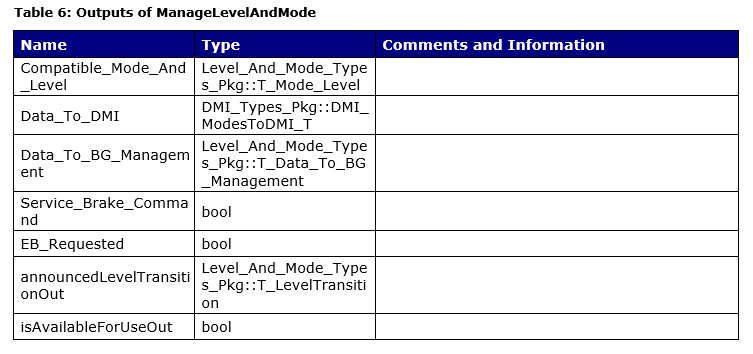
\includegraphics[width=\textwidth]{images/Outputs_ML.png}
\caption{Mode\_and\_Level outputs}\label{f:mode_and_level_outputs}
\end{figure}



\paragraph{Compatible\_Mode\_And\_Level}

\begin{longtable}{p{.25\textwidth}p{.7\textwidth}}
\toprule
Output name				& Compatible\_Mode\_And\_Level \\
\midrule
Description				& Structure containing mode and level information.  \\
\midrule
Destination				& F2.1 Manage\_TrackSideInformation\_Integration\newline
F2.4 TrackAtlas\newline
F2.8 ProvidePositionReport\newline
F2.9 MoRC\_Main\newline
F2.11 manageDMI\_output\newline 
F2.13 manageTIU\_output \\ 
\midrule
Type					& Level\_And\_Mode\_Types\_Pkg::T\_Mode\_Level \\
\midrule
Valid range of values	& It is a complex type: 
\begin{itemize}
\item CompatibleModeAndLevel : bool,
\item level : M\_LEVEL,
\item newLevel : bool,
\item mode : M\_MODE, 
\item newMode : bool
\end{itemize} \\
\midrule
Behaviour when value is at boundary	& n/a \\ 
\midrule
Behaviour for values out of valid range	& n/a \\ 
\midrule
Behaviour when value is erroneous, absent or unwanted (i.e. spurious) & n/a \\
\bottomrule
\end{longtable}

\paragraph{Data\_To\_DMI\_Ack}

\begin{longtable}{p{.25\textwidth}p{.7\textwidth}}
\toprule
Output name				& Data\_To\_DMI\_Ack \\
\midrule
Description				& Data information to provided to the driver.  \\
\midrule
Destination				& F2.11 manageDMI\_output  \\ 
\midrule
Type					& DMI\_Types\_Pkg::DMI\_ModesToDMI\_T \\
\midrule
Valid range of values	& It is a complex type defined in the DMI package. \\
\midrule
Behaviour when value is at boundary	& n/a \\ 
\midrule
Behaviour for values out of valid range	& n/a \\ 
\midrule
Behaviour when value is erroneous, absent or unwanted (i.e. spurious) & n/a \\
\bottomrule
\end{longtable}

\paragraph{Data\_To\_BG\_Management}

\begin{longtable}{p{.25\textwidth}p{.7\textwidth}}
\toprule
Output name				& Data\_To\_BG\_Management \\
\midrule
Description				& Set of data concerning BG management. \\
\midrule
Destination				& This output is currently not used in the model.  \\ 
\midrule
Type					& Level\_And\_Mode\_Types\_Pkg::T\_Data\_To\_BG\_Management \\
\midrule
Valid range of values	& It is a complex type:
\begin{itemize}
\item EoM\_Procedure\_req : bool,
\item  Clean\_BG\_List\_SH\_Area : bool, 
\item MA\_Req : bool,
\item  Req\_for\_SH\_from\_Driver : bool,
\item Connection\_to\_RBC\_req : bool, 
\item Position\_Repport\_Needed : bool
\end{itemize} \\
\midrule
Behaviour when value is at boundary	& n/a \\ 
\midrule
Behaviour for values out of valid range	& n/a \\ 
\midrule
Behaviour when value is erroneous, absent or unwanted (i.e. spurious) & n/a \\
\bottomrule
\end{longtable}


\paragraph{Service\_Brake\_Command}

\begin{longtable}{p{.25\textwidth}p{.7\textwidth}}
\toprule
Output name				& Service\_Brake\_Command \\
\midrule
Description				& Command for the service brake. \\
\midrule
Destination				& F2.7 SpeedSupervision\_Integration \\ 
\midrule
Type					& bool \\
\midrule
Valid range of values	&  
\begin{description}
\item[true] Service brake shall be applied.
\item[false] Service brake shall not be applied.
\end{description}\\
\midrule
Behaviour when value is at boundary	& n/a \\ 
\midrule
Behaviour for values out of valid range	& n/a \\ 
\midrule
Behaviour when value is erroneous, absent or unwanted (i.e. spurious) & n/a \\
\bottomrule
\end{longtable}

\paragraph{EB\_Requested}

\begin{longtable}{p{.25\textwidth}p{.7\textwidth}}
\toprule
Output name				& EB\_Requested \\
\midrule
Description				& Command of the emergency brake \\
\midrule
Destination				& F2.7 SpeedSupervision\_Integration \\ 
\midrule
Type					& bool \\
\midrule
Valid range of values	&  
\begin{description}
\item[true] Emergency brake shall be applied.
\item[false] Emergency brake shall not be applied.
\end{description}\\
\midrule
Behaviour when value is at boundary	& n/a \\ 
\midrule
Behaviour for values out of valid range	& n/a \\ 
\midrule
Behaviour when value is erroneous, absent or unwanted (i.e. spurious) & n/a \\
\bottomrule
\end{longtable}



\paragraph{announcedLevel}

\begin{longtable}{p{.25\textwidth}p{.7\textwidth}}
\toprule
Input name				& announcedLevel \\
\midrule
Description				& Level transition selected for an immediate or future transition. \\
\midrule
Destination				& F2.7 SpeedSupervision\_Integration \\ 
\midrule
Type					& Level\_And\_Modes\_Types\_Pkg::T\_LevelTransition \\
\midrule
Valid range of values	& It is a complex type:  
\begin{itemize}
\item is\_set : bool,
\item transition : Level\_And\_Mode\_Types\_Pkg::T\_LevelTansitionInfo, 
\item LRBG : NID\_LRBG, 
\item referenceLocation : Obu\_BasicTypes\_Pkg::L\_internal\_Type
\end{itemize} \\
\midrule
Behaviour when value is at boundary	& n/a \\ 
\midrule
Behaviour for values out of valid range	& n/a \\ 
\midrule
Behaviour when value is erroneous, absent or unwanted (i.e. spurious) & n/a \\ 
\bottomrule \\ 
\end{longtable}





\subsection{Subcomponents}\label{s:mdoe_and_level_subcomponents}

\subsubsection{Level\_Management}
%set the master document for easy compilation
%!TEX root = ../D3_5_3.tex

\paragraph{Component Requirements}

\begin{longtable}{p{.25\textwidth}p{.7\textwidth}}
\toprule
Component name			& Level\_Management \\
\midrule
Link to SCADE model		& {\footnotesize \url{https://github.com/openETCS/modeling/tree/master/model/Scade/System/ObuFunctions/ManageLevelsAndModes/Levels}} \\
\midrule
SCADE designer			& Marielle Petit-Doche and  Matthias G\"udemann, Systerel \\
\midrule
Description				& The level management subsystem receives level transition order tables and selects the order with the highest probability. It stores the information about the selected transition order and transits to the requested level once the train passes the location of the level transition.

If required, the driver is asked to acknowledge the transition, in case of no acknowledgment or if conditions for the level transition are not fulfilled, the train gets tripped.

On the most abstract level the design consists of the \emph{manage\_priorities} function which takes the level transition order priority tables as inputs and computes the highest priority transition.

This transition order is the fed to the \emph{computeLevelTransitions} operator. This operator consists of three main parts. The \emph{ComputeTransitionConditions} operator that emits the fulfilled conditions to change from a given level to a new level, the \emph{LevelStateMachine} that stores the current level and takes the computed change conditions as input for possible level transitions and finally the \emph{driverAck} operator which contains a state machine that stores the information whether the system is currently waiting for a driver acknowledge and emits the train trip information if necessary. \\
\midrule
Input documents	& 
Subset-026, Chapter 5.10 \\
\midrule
Safety integrity level		& 4 \\
\midrule
Time constraints		& n/a \\
\midrule
API requirements 		&  n/a \\
\bottomrule
\end{longtable}


\paragraph{Interface}

For an overview of the interface of this internal component we refer to the SCADE model (cf.~link above) respectively the SCADE generated documentation \url{https://github.com/openETCS/modeling/blob/master/model/Scade/System/ObuFunctions/ManageLevelsAndModes/Levels/Levels.rtf}

\subsubsection{Mode\_Management}
%set the master document for easy compilation
%!TEX root = ../D3_5_3.tex

\paragraph{Component Requirements}

\begin{longtable}{p{.25\textwidth}p{.7\textwidth}}
\toprule
Component name			& Mode\_Management \\
\midrule
Link to SCADE model		& {\footnotesize \url{https://github.com/openETCS/modeling/tree/master/model/Scade/System/ObuFunctions/ManageLevelsAndModes/Modes}} \\
\midrule
SCADE designer			& Marielle Petit-Doche, Systerel \\
\midrule
Description				& This function is in charge of the computation of new mode to apply according to conditions from inputs (track information, driver interactions, train data,...) and other functions.

Three subfunctions are defined:
\begin{description}
\item[Inputs] proceeds to inputs check and preparation.
\item[ComputeModesCondition] performs all specific procedure linked to mode management and defined in  \citep{subset-026} sections 5.4, 5.5, 5.6, 5.7, 5.8, 5.9, 5.11, 5.12, 5.13, 5.19 and specifies the conditions to define a mode transition according condition table of section 4.6.3 of \citep{subset-026}
\item[SwitchModes] performs the mode selection according the conditions and priorities defined in transition table  section 4.6.2 of \citep{subset-026}
\item[Outputs] prepares packet of outputs.
\end{description} \\
\midrule
Input documents	& 
Subset-026, Chapter 4.4, 4.6, 5.4, 5.5, 5.6, 5.7, 5.8, 5.9, 5.11, 5.12, 5.13, 5.19 \\
\midrule
Safety integrity level		& 4 \\
\midrule
Time constraints		& n/a \\
\midrule
API requirements 		&  n/a \\
\bottomrule
\end{longtable}


\paragraph{Interface}

For an overview of the interface of this internal component we refer to the SCADE model (cf.~link above) respectively the SCADE generated documentation \url{https://github.com/openETCS/modeling/blob/master/model/Scade/System/ObuFunctions/ManageLevelsAndModes/Modes/Modes.pdf}

\subsubsection{Check\_and\_Provide\_Mode\_and\_Level}
%set the master document for easy compilation
%!TEX root = ../D3_5_3.tex

\paragraph{Component Requirements}

\begin{longtable}{p{.25\textwidth}p{.7\textwidth}}
\toprule
Component name			& Check\_and\_Provide\_Mode\_and\_Level \\
\midrule
Link to SCADE model		& {\footnotesize \url{https://github.com/openETCS/modeling/tree/master/model/Scade/System/ObuFunctions/ManageLevelsAndModes/ModesAndLevels}} \\
\midrule
SCADE designer			& Marielle Petit-Doche, Systerel \\
\midrule
Description				& Checks compatibility between mode and level and provides outputs. \\
\midrule
Input documents	& 
Subset-026, Chapter 3.6.5 \\
\midrule
Safety integrity level		& 4 \\
\midrule
Time constraints		&  n/a \\
\midrule
API requirements 		&  n/a \\
\bottomrule
\end{longtable}


\paragraph{Interface}

For an overview of the interface of this internal component we refer to the SCADE model (cf.~link above) respectively the SCADE generated documentation.




%set the master document for easy compilation
%!TEX root = ../D3_5_3.tex

\section{F2.6: calculateTrainPosition}\label{s:F2.6}

\subsection{Component Requirements}

\begin{longtable}{p{.25\textwidth}p{.7\textwidth}}
\toprule
Component name			& calculateTrainPosition \\
\midrule
Link to SCADE model		& {\footnotesize \url{https://github.com/openETCS/modeling/tree/master/model/Scade/System/ObuFunctions/ManageLocationRelatedInformation/TrainPosition/CalculateTrainPosition}} \\
\midrule
SCADE designer			& Uwe Steinke, Siemens AG \\
\midrule
Description				& The main purpose of the function is to calculate the locations of linked and unlinked balise groups (BGs) and the current train position while the train is running along the track. In detail, the calculateTrainPosition function provides a couple of essential subfunctions for the onboard unit. These are mainly:
\begin{itemize}
\item Creating and maintaining an obu internal coordinate system for all types of location based data.
\item Storing all linked and unlinked balise groups resulting from over passing or from announcements (linking information) from the track.
\item Calculating and maintaining the locations of all stored balise groups during the train trip, based on odometry and linking information.
\item Permanently calculating the current train position based on odometry and passed balise group information.
\item Providing the last recently passed linked balise group as the LRBG.
\item Providing additional position attribute information.
\item Deleting stored balise groups, when appropriate.
\item Detecting linking consistency errors.
\item Determining, if linking is used on board.
\end{itemize}
The calculation algorithms for locations and positions are implemented as specified in 
{\footnotesize\url{https://github.com/openETCS/SRS-Analysis/blob/master/System%20Analysis/WorkingRepository/Group4/SUBSET_26_3-6/DetermineTrainLocationProcedures.pdf}} \\
\midrule
Input documents	& 
Subset-026, Chapter 3.6 \\
\midrule
Safety integrity level	& 4 \\
\midrule
Time constraints		& All events at the calculateTrainPosion inputs must be applied strictly in the correct chronological order. \\
\midrule
API requirements 		& The currentOdometry input as well as the odometry stamps within msgFromTrack  must be fed with odometry values strictly adhering to {\footnotesize\url{https://github.com/openETCS/SRS-Analysis/blob/master/System%20Analysis/WorkingRepository/Group4/SUBSET_26_3-6/DetermineTrainLocationProcedures.pdf}}, chapt. 3.
 \\
\bottomrule
\end{longtable}


\subsection{Interface}

An overview of the interface of component calculateTrainPosition is shown in Figure~\ref{f:calculateTrainPosition_interface}. The inputs and outputs are described in detail in Section~\ref{s:calculateTrainPosition_inputs} respectively \ref{s:calculateTrainPosition_outputs}. Subcomponents are described in Section~\ref{s:calculateTrainPosition_subcomponents}.


\begin{figure}
	\centering
	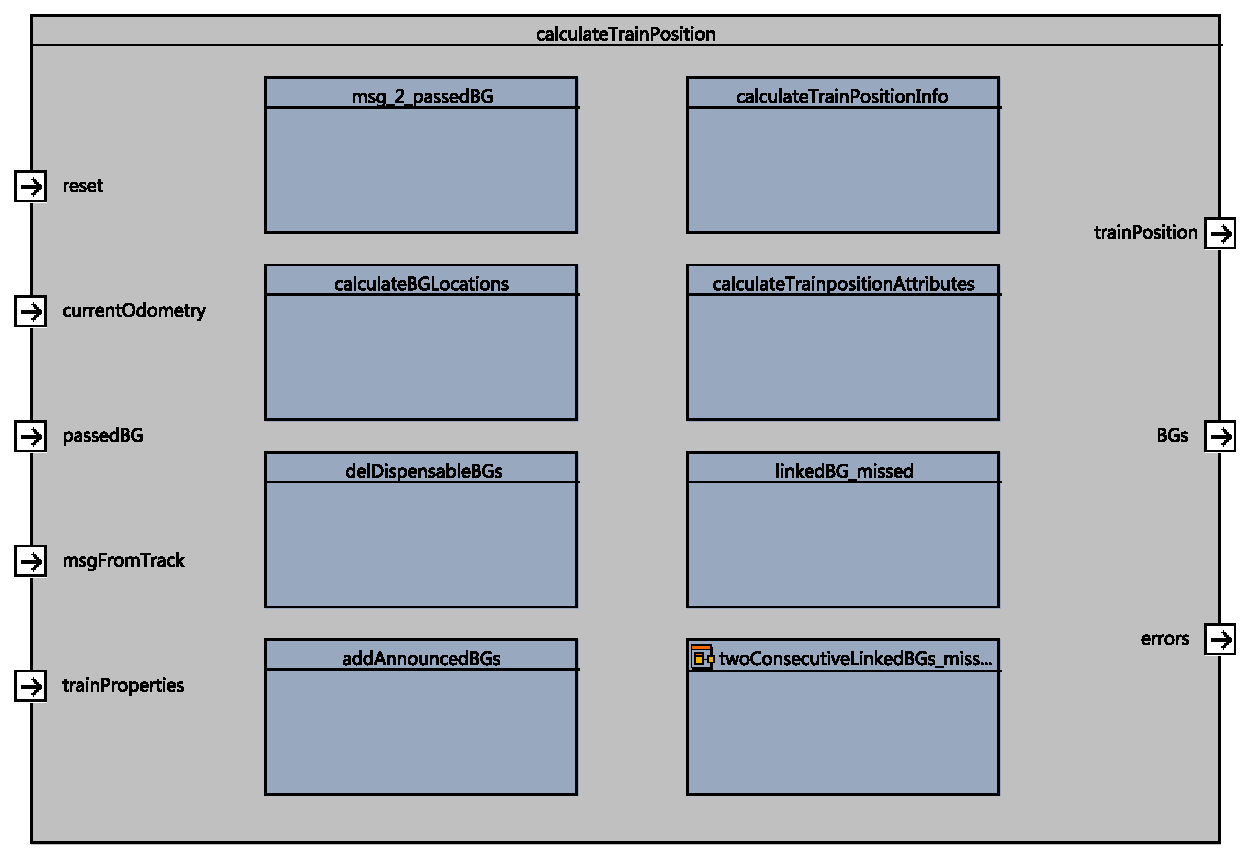
\includegraphics[width=\textwidth]{./images/F2_6_calculateTrainPosition.pdf}
	\caption{calculateTrainPosition component SysML diagram.}
	\label{fig:calculateTrainPosition_interface}
\end{figure}


\subsubsection{Inputs}\label{s:calculateTrainPosition_inputs}

\paragraph{currentOdometry}

\begin{longtable}{p{.25\textwidth}p{.7\textwidth}}
\toprule
Input name				& currentOdometry \\
\midrule
Description				& currentOdometry is the actual odometry information as known by the whole EVC model and provided by the models external interface. \\
\midrule
Source					& F2 input API\_Odometry \\ 
\midrule
Type					& Obu\_BasicTypes\_Pkg::odometry\_T \\  
\midrule
Valid range of values	& Obu\_BasicTypes\_Pkg::odometry\_T is a complex data type. Values are given for each element. Format is: Type Name: range / list of values.
\begin{itemize}
\item bool valid: [true | false]. Must be permanently set to "true".
\item timestamp: (0 - 2147483647). Current time in ms, must be monotonically increasing.
\item odo: Obu\_BasicTypes\_Pkg::OdometryLocations\_T: current odometry log values with uncertainties; must behave according to {\footnotesize\url{https://github.com/openETCS/SRS-Analysis/blob/master/System%20Analysis/WorkingRepository/Group4/SUBSET_26_3-6/DetermineTrainLocationProcedures.pdf}} [[ 3.1 ]]. Members of OdometryLocations\_T are: 
  \begin{itemize}
  \item o\_nominal: L\_internal\_Type: nominal value in cm.
  \item o\_min:     L\_internal\_Type: \newline min. distance = o\_min2 - o\_min1
  \item o\_max:     L\_internal\_Type: \newline max distance = o\_max2 - o\_max1
  \end{itemize}
\item speed: Obu\_BasicTypes\_Pkg::OdometrySpeeds\_T: not used by calculateTrainPosition
\item acceleration: Obu\_BasicTypes\_Pkg::A\_internal\_Type: not used by calculateTrainPosition
\item motionState: [noMotion | Motion]
\item motionDirection: Obu\_BasicTypes\_Pkg::odoMotionDirection\_T \newline [ unknownDirection | cabAFirst | cabBFirst ]
\end{itemize}
\emph{calculateTrainPosition requires consistent value sets of currentOdometry. calculateTrainPosition itself does not check.  }\\
\midrule
Behaviour when value is at boundary	& n/a \\
\midrule
Behaviour for values out of valid range	& Enumerated values out of range prohibit code generation. In all other cases, calculateTrainPosition does not have the knowledge for out-of-range checks. \\
\midrule
Behaviour when value is erroneous, absent or unwanted (i.e. spurious) & Leads to misbehaviour. \\
\bottomrule
\end{longtable}



\paragraph{msgFromTrack}

\begin{longtable}{p{.25\textwidth}p{.7\textwidth}}
\toprule
Input name				& msgFromTrack \\
\midrule
Description				& With msgFromTrack calculateTrainPosition receives datagrams from balise groups and RBC. \\
\midrule
Source					& F2.1 Manage\_TrackSideInformation\_Integration \\ 
\midrule
Type					& Common\_Types\_Pkg::ReceivedMessage\_T \\  
\midrule
Valid range of values	& Common\_Types\_Pkg::ReceivedMessage\_T is a complex data type. Values are given for each element. Format is: Type Name: range / list of values.
\begin{itemize}
	\item bool valid: [true | false]. "true" flags a datagram as received and to be evaluated by calculateTrainPosition. Must be set for exactly 1 clock for each received datagram and stay unset otherwise.

	\item source: Common\_Types\_Pkg::MsgSource\_T: Designates the source of the datagram: \newline ( msrc\_undefined | msrc\_Euroradio | msrc\_Eurobalise | msrc\_RadioInfillUnit | msrc\_OBU ) 

	\item radioMetaData: Common\_Types\_Pkg::radioMetaData\_T: not used by calculateTrainPosition.

	\item BG\_Common\_Header: BG\_Types\_Pkg::BG\_Header\_T: Header information received from balise groups, refer to Manage\_TrackSideInformation\_Integration\_Pkg::\newline Manage\_TrackSideInformation\_Integration

	\item Radio\_Common\_Header: Radio\_Types\_Pkg::Radio\_TrackTrain\_Header\_T: Header information received from RBC via radio, refer to Manage\_TrackSideInformation\_Integration\_Pkg::\newline Manage\_TrackSideInformation\_Integration

	\item packets: Common\_Types\_Types\_Pkg::CompressedPackets\_T: datagram packets, refer to Manage\_TrackSideInformation\_Integration\_Pkg::\newline Manage\_TrackSideInformation\_Integration. calculatesTrainPosition extracts packet 5 (linking information), if available.

	\item sendingRBC: Common\_Types\_Types\_Pkg::RBC\_Id\_T: designates the origin RBC and the mobile modem channel used onboard, if received via radio. Refer to Manage\_TrackSideInformation\_Integration\_Pkg::\newline Manage\_TrackSideInformation\_Integration for more detailed information.
\end{itemize}  
\emph{calculateTrainPosition expects the received information to be consistent and validated before applied to. It does not check, if the information is appropriate due to current EVC mode, level, train or balise orientation. Received balise group or linking information already known by calculateTrainPosition overrides former data. All messages must be applied in the correct chronological order} \\
\midrule
Behaviour when value is at boundary	& n/a \\
\midrule
Behaviour for values out of valid range	& Enumerated values out of range prohibit code generation. In all other cases, calculateTrainPosition does not have the knowledge for out-of-range checks. \\
\midrule
Behaviour when value is erroneous, absent or unwanted (i.e. spurious) & Causes misbehaviour.
\\
\bottomrule
\end{longtable}


\paragraph{trainProperties}

\begin{longtable}{p{.25\textwidth}p{.7\textwidth}}
\toprule
Input name				& trainProperties \\
\midrule
Description				& Supplies calculateTrainPosition with train specific properties required for position calculation.   \\
\midrule
Source					& F2.3 trainData\newline
F2.10 manageDMI\_input \\ 
\midrule
Type					& TrainPosition\_Types\_Pck::trainProperties\_T \\  
\midrule
Valid range of values	& TrainPosition\_Types\_Pck::trainProperties\_T is a complex data type. Values are given for each element. Format is: Type Name: range / list of values.
\begin{itemize}
\item nid\_engine:: NID\_ENGINE as defined by subset 026-7. 
\item nid\_operational: NID\_OPERATIONAL as defined by subset 026-7. 
\item l\_train: L\_TRAIN as defined by subset 026-7. 
\item d\_baliseAntenna\_2\_frontend: Obu\_BasicTypes\_Pkg::LocWithInAcc\_T:  Distance from the trains balise antenna to the trains front end, in cm with uncertainties. 
\item d\_frontend\_2\_rearend: Obu\_BasicTypes\_Pkg::LocWithInAcc\_T:  Distance from the trains Distance from the trains front end to rear end, in cm with uncertainties. 
\item locationAccuracy\_DefaultValue: Obu\_BasicTypes\_Pkg::LocWithInAcc\_T:  Default location accuracy of balise groups (subset 026, 3.6.4.3.2), in cm with uncertainties. 
\item centerDetectionAcc\_DefaultValue: Obu\_BasicTypes\_Pkg::LocWithInAcc\_T:  Default  accuracy of balise groups detection of the BTM, in cm with uncertainties. Will be applied, if centerDetectionInaccuracy from BTM is not available, especially for announced and not yet passed BGs. 
\end{itemize} 
\emph{calculateTrainPosition expects this information to be consistent and validated before applied to.}\\
\midrule
Behaviour when value is at boundary	& n/a \\
\midrule
Behaviour for values out of valid range	& Enumerated values out of range prohibit code generation. In all other cases, calculateTrainPosition does not have the knowledge for out-of-range checks. \\
\midrule
Behaviour when value is erroneous, absent or unwanted (i.e. spurious) & Causes misbehaviour.
\\
\bottomrule
\end{longtable}



\paragraph{passedBG}

\begin{longtable}{p{.25\textwidth}p{.7\textwidth}}
\toprule
Input name				& passedBG \\
\midrule
Description				& Deprecated alternative input to msgFromTrack. Must not be used any more and is subject to be removed in subsequent releases.  \\
\bottomrule
\end{longtable}


\paragraph{reset}

\begin{longtable}{p{.25\textwidth}p{.7\textwidth}}
\toprule
Input name				& reset \\
\midrule
Description				& Resets and keeps calculateTrainPosition at its initial state and deletes all internally stored data.  \\
\midrule
Source					& F2 input EVC\_reset \\ 
\midrule
Type					& bool \\  
\midrule
Valid range of values	& [ false | true ] \\
\midrule
Behaviour when value is at boundary	& n/a \\
\midrule
Behaviour for values out of valid range	& Enumerated values out of range prohibit code generation. \\
\midrule
Behaviour when value is erroneous, absent or unwanted (i.e. spurious) & Causes misbehaviour.
\\
\bottomrule
\end{longtable}


\subsubsection{Outputs}\label{s:calculateTrainPosition_outputs}

\paragraph{trainPosition}

\begin{longtable}{p{.25\textwidth}p{.7\textwidth}}
\toprule
Output name				& trainPosition \\
\midrule
Description				& Provides the current train position and LRBG with its attributes. All distance and location computations of the OBU must be based on this information.   \\
\midrule
Destination				& F2.1 Manage\_TracksideInformation\_Integration\newline
F2.2 Manage\_ETCS\_Procedures\newline
F2.4 TrackAtlas\newline
F2.5 ManageLevelAndMode\newline
F2.7 PeedSupervision\_Integration\newline
F2.8 ProvidePositionReport\newline
F2.11 manageDMI\_Output
\\ 
\midrule
Type					& TrainPosition\_Types\_Pck::trainPosition\_T \\  
\midrule
Valid range of values	& TrainPosition\_Types\_Pck::trainPosition\_T is a complex data type. Values are given for each element. Format is: Type Name: range / list of values.
\begin{itemize}
\item valid: bool: [true | false]. Always true, except for exceptional circumstances.
\item timestamp: Obu\_BasicTypes\_Pkg::T\_internal\_Type: latest time in ms. 
\item trainPositionIsUnknown: bool: true, if the train position is evaluated as "unknonwn" (refer to subset-026, 3.6.3.1.3.1). 
\item noCoordinateSystemHasBeenAssigned: bool: refer to subset 026, 3.4.2, 3.6.3.1.4.
\item trainPosition: Obu\_BasicTypes\_Pkg::LocWithInAcc\_T: The calculated train position with uncertainties
\item estimatedFrontEndPosition: Obu\_BasicTypes\_Pkg::Location\_T: Train front end position in cm.
\item minSafeFrontEndPosition: Obu\_BasicTypes\_Pkg::Location\_T: Train front end position in cm.
\item maxSafeFrontEndPostion: Obu\_BasicTypes\_Pkg::Location\_T: Train front end position in cm.
\item LRBG: TrainPosition\_Types\_Pck::positionedBG\_T: the current LRBG. 
\item prvLRBG: TrainPosition\_Types\_Pck::positionedBG\_T: the balise group passed previously to LRBG. For type definition, see below.
\item nominalOrReverseToLRBG: Q\_DLRBG: Orientation of the train in relation to the direction of the LRBG, see subset 026-7.
\item trainOrientationToLRBG: Q\_DIRLRBG: Orientation of the train in relation to the direction of the LRBG, see subset 026-7.
\item trainRunningDirectionToLRBG: Q\_DIRTRAIN: Direction of train movement in relation to the LRBG orientation, see subset 026-7.
\item linkingIsUsedOnboard: bool: Designates, if at least one announced linked BG is ahead.
\end{itemize} 
\emph{calculateTrainPosition provides the train position to whom it concerns and recalculates it in every clock cycle.} \\
\midrule
Behaviour when value is at boundary	& n/a \\
\midrule
Behaviour for values out of valid range	& n/a \\
\midrule
Behaviour when value is errorneous, absent or unwanted & n/a \\
\bottomrule
\end{longtable}


\paragraph{BGs}

\begin{longtable}{p{.25\textwidth}p{.7\textwidth}}
\toprule
Output name				& BGs \\
\midrule
Description				& A list of all linked and unlinked balise groups - known to calculateTrainPosition - in the order they are arranged on the track.   \\
\midrule
Destination				& F2.1 Manage\_TracksideInformation\_Integration\newline
F2.8 ProvidePositionReport \\ 
\midrule
Type					& array of TrainPosition\_Types\_Pck::positionedBG\_T \\  
\midrule
Valid range of values	& TrainPosition\_Types\_Pck::positionedBG\_T is a complex data type. Values are given for each array element. Format is: Type Name: range / list of values.
\begin{itemize}
	\item valid: bool: [true | false]. "true" for every existing balise group.
	\item nid\_c: NID\_C: refer to subset 026-7. 
	\item nid\_bg: NID\_BG: refer to subset 026-7. 
	\item q\_link: Q\_LINK: refer to subset 026-7. 
	\item location: Obu\_BasicTypes\_Pkg::LocWithInAcc\_T: The best known location (with inaccuracies) calculated from linking and from passing information.
	\item seqNoOnTrack: int: Sequence number, specifies the order of the BG passed or expected to be passed.
	\item infoFromLinking: TrainPosition\_Types\_Pck::infoFromLinking\_T: Describes a linked BG as announced from the linking BG. Mainly, this information is taken from the linking packet.
	\item infoFromPassing: BG\_Types\_Pkg::passedBG\_T: If the balise group has been passed already, this is the relevant information received from the BG.
\end{itemize} 
\emph{calculateTrainPosition provides the list of balise groups to whom it concerns.}\\
\midrule
Behaviour when value is at boundary		& n/a \\
\midrule
Behaviour for values out of valid range	& n/a \\
\midrule
Behaviour when value is errorneous, absent or unwanted & n/a \\
\bottomrule
\end{longtable}


\paragraph{errors}

\begin{longtable}{p{.25\textwidth}p{.7\textwidth}}
\toprule
Output name				& errors \\
\midrule
Description				& Provides a collection of error flags, raised by calculateTrainPosition.   \\
\midrule
Destination				& F2.5 ManageLevelAndMode\newline
F2.8 ProvidePositionReport \\ 
\midrule
Type					& TrainPosition\_Types\_Pck::positionErrors\_T \\  
\midrule
Valid range of values	& TrainPosition\_Types\_Pck::positionErrors\_T is a complex data type. Values are given for each array element. Format is: Type Name: range / list of values.
\begin{itemize}
\item outOfMemSpace: bool: Memory overrun: a passed or announced BG could not be stored.
\item passedBG\_foundNotWhereExpected: bool: The currently passed linked BG location does not match its expectation window.
\item positionCalculation\_inconsistent: A consistency problem arose during position calculation.
\item linkedBGMissed: bool: The expectation window for an announced BG was passed without detecting the BG.
\item BGpassedInUnexpectedDirection: bool: The BG was passed in a different orientation than announced via linking.
\item BG\_LinkingConsistencyError: bool: Linking consistency error (ref. subset 026, 3.16.2.3).
\item twoConsecutiveLinkedBGs\_missed: bool: 2 consecutive linked balise groups announced by linking are not detected and the end of the expectation window of the second balise group has been passed (subset 026, 3.16.2.7.1).
\item doubleRepositioningError: bool: Double repositioning error (3.16.2.7.2).
\item bg: TrainPosition\_Types\_Pck::positionedBG\_T: The corresponding balise group in the case of an error.
\end{itemize}  \\
\midrule
Behaviour when value is at boundary		& n/a \\
\midrule
Behaviour for values out of valid range	& n/a \\
\midrule
Behaviour when value is errorneous, absent or unwanted & n/a \\
\bottomrule
\end{longtable}


\subsection{Subcomponents}\label{s:calculateTrainPosition_subcomponents}

\subsubsection{msg\_2\_passedBG}
\input{sections/msg_2_passedBG}

\subsubsection{calculateBGLocations}
\input{sections/calculateBGLocations}

\subsubsection{delDispensableBGs}
\input{sections/delDispensableBGs}

\subsubsection{addAnnouncedBGs}
\input{sections/addAnnounceBGs}

\subsubsection{calculateTrainpositionInfo}
\input{sections/calculateTrainpositionInfo}

\subsubsection{calculateTrainPositionAttributes}
\input{sections/calculateTrainPositionAttributes}

\subsubsection{linkedBG\_missed}
\input{sections/linkedBG_missed}

\subsubsection{twoconsecutiveLinkedBGs\_missed}
\input{sections/twoconsecutiveLinkedBGs_missed}








%set the master document for easy compilation
%!TEX root = ../D3_5_3.tex

\section{F2.7: SpeedSupervision\_Integration}\label{s:F2.7}

\subsection{Component Requirements}

\begin{longtable}{p{.25\textwidth}p{.7\textwidth}}
\toprule
Component name			& SpeedSupervision\_Integration\\
\midrule
Link to SCADE model		& {\footnotesize \url{https://github.com/openETCS/modeling/tree/master/model/Scade/System/ObuFunctions/SpeedSupervison}} \\
\midrule
SCADE designer			& Benjamin Beichler, University of Rostock\newline
Christian Stahl, TWT\newline
Thorsten Schulz, University of Rostock \\
\midrule
Description				& The task of SDM is to monitor the speed of the train and the train location and as such to ensure that the speed remains within the given speed and distance limits. This block is based on \cite[Chapt.~3.13]{subset-026}.

The integration node ``SpeedSupervision\_Integration'' takes as input (1) movement related information such as train speed, train position and acceleration, (2) train related information such as brake information and train length, and (3) track related information such as speed and distance limits and national values.

Based on this information a speed profile is calculated. Speed restrictions create target speeds (targets) that have to be followed. For each such target braking curves are generated to supervise at which location of the track the train must apply the brake. In case of no target restrictions the train may accelerate to the supervised maximum speed of the speed profile. These calculations lead to commands being sent to the driver and the brake system.

The functionality is modeled using eight subcomponents, as shown in Figure~\ref{f:ssv}, which are explained in Section~\ref{s:SDM_subcomponents}.

The current status of the analysis of ``SDM'' and a functional breakdown can be found in a separate document, \verb+SpeedSupervision_analysis.pdf+.\\
\midrule
Input documents	& 
Subset-026, Chapter 3.13: Speed and distance monitoring \\
\midrule
Safety integrity level		& 4 \\
\midrule
Time constraints		& n/a \\
\midrule
API requirements 		& n/a \\
\bottomrule
\end{longtable}


\subsection{Interface}

An overview of the interface of component SpeedSupervision\_integration is shown in Figure~\ref{f:ssv}. The inputs and outputs are described in detail in Section~\ref{s:SDM_inputs} respectively \ref{s:SDM_outputs}. Sub components are described in Section~\ref{s:SDM_subcomponents}.

\begin{figure}
\centering
\includegraphics[width=0.95\textheight, angle=90]{../images/speedsupervision.png}
\caption{Structure of component SpeedSupervision\_Integration.}\label{f:ssv}
\end{figure}



\subsubsection{Inputs}\label{s:SDM_inputs}

\paragraph{National Values}

\begin{longtable}{p{.25\textwidth}p{.7\textwidth}}
\toprule
Input name				& NationalValues \\
\midrule
Description				& This input is packet 3 or 203 of \cite[Chapt.~8]{subset-026}, describing the national values.  \\
\midrule
Source					& TrackAtlas; current release, hard wired constant: cP3NationalValuesUtrechtAmsterdam \\
\midrule
Type					& P3\_NationalValues\_T \\
\midrule
Valid range of values	& P3\_NationalValues\_T is a complex data type, valid ranges are specified in SRS Subset-026-7, no further checks are done here. \\
\midrule
Behaviour when value is at boundary	& n/a \\
\midrule
Behaviour for values out of valid range	& n/a \\
\midrule
Behaviour when value is erroneous, absent or unwanted (i.e. spurious) & Not checked; node must not be called without reasonable National Value. \\
\bottomrule
\end{longtable}


\paragraph{Train Position}

\begin{longtable}{p{.25\textwidth}p{.7\textwidth}}
\toprule
Input name				& TrainPosition \\
\midrule
Description				& This input is the current train position. \\
\midrule
Source					& calculateTrainPosition \\
\midrule
Type					& trainPosition\_T \\
\midrule
Valid range of values	& trainPosition\_T is a complex data type. Value valid must not be false for proper function and it may not be properly checked in current release. Furthermore, reversing (decreasing positions, reverse flag set) is currently NOT supported and leads to undefined behaviour. No brake will be thrown in this occasion.
\todo[inline]{To be completed}\\
\midrule
Behaviour when value is at boundary	& Not checked, may overflow. \\
\midrule
Behaviour for values out of valid range	& Currently not checked. \\
\midrule
Behaviour when value is erroneous, absent or unwanted (i.e. spurious) & Not checked; node must not be called without reasonable position data. Valid flag is not checked (bug), as SDM has not yet implemented exception handling on inacceptable input data. \\
\bottomrule
\end{longtable}


\paragraph{Odometry}

\begin{longtable}{p{.25\textwidth}p{.7\textwidth}}
\toprule
Input name				& odometry \\
\midrule
Description				& This input is the odometry data. \\
\midrule
Source					& API\_Odometry \\ 
\midrule
Type					& odometry\_T \\
\midrule
Valid range of values	& complex data type \\
 & used fields are: \\
 & - acceleration: Obu\_BasicTypes\_Pkg::A\_internal\_Type. No valid range defined, neither checked. \\
 & - motionState: [noMotion | Motion] (enum type) \\
 & - motionDirection: is NOT evaluated currently which leads to erroneous behaviour when driving anti-nominal direction.\\
\midrule
Behaviour when value is at boundary	& Possible overflow not evaluated. \\
\midrule
Behaviour for values out of valid range	& Not checked. \\
\midrule
Behaviour when value is erroneous, absent or unwanted (i.e. spurious) & Not handled, valid data is expected for valid function. Valid flag is not checked (bug), as SDM has not yet implemented exception handling on inacceptable input data.\\
\bottomrule
\end{longtable}


\paragraph{Train Properties}

\begin{longtable}{p{.25\textwidth}p{.7\textwidth}}
\toprule
Input name				& trainProps \\
\midrule
Description				& This input is a set of train related properties. \\
\midrule
Source					& maintainTrainProperties \\ 
\midrule
Type					& trainProperties\_T \\
\midrule
Valid range of values	& trainProperties\_T is a complex type but referenced only d\_baliseAntenna\_2\_frontend.nominal: Obu\_BasicTypes\_Pkg::L\_internal\_Type No valid range defined, neither checked. \\
\midrule
Behaviour when value is at boundary	& n/a \\
\midrule
Behaviour for values out of valid range	& n/a \\
\midrule
Behaviour when value is erroneous, absent or unwanted (i.e. spurious) & Value is only evaluated in Level 1. Low values (e.g. invalid-default 0) will lead to early trip, brake and alike. Larger values will lead to late braking, possibly numeric overflow. \\
\bottomrule
\end{longtable}


\paragraph{Train Data}

\begin{longtable}{p{.25\textwidth}p{.7\textwidth}}
\toprule
Input name				& trainData \\
\midrule
Description				& This input is a set of train related inputs from the TIU. \\
\midrule
Source					& manageTrainData \\ 
\midrule
Type					& trainData\_T \\
\midrule
Valid range of values	& trainData\_T is a complex type. No valid range defined, neither checked. The source is trusted. \\
\midrule
Behaviour when value is at boundary	& n/a \\
\midrule
Behaviour for values out of valid range	& n/a \\
\midrule
Behaviour when value is erroneous, absent or unwanted (i.e. spurious) & Must be valid for SDM to function. Valid flag is not checked (bug), as SDM has not yet implemented exception handling on inacceptable input data. \\
\bottomrule
\end{longtable}

\paragraph{Track Data}

\begin{longtable}{p{.25\textwidth}p{.7\textwidth}}
\toprule
Input name				& dataFromTrackAtlas \\
\midrule
Description				& This input is a set of track related input data, containing the MRSP, the Gradient Profile and the Movement Authority. And its associated update flags to opimize data handling.\\
\midrule
Source					& TrackAtlas \\ 
\midrule
Type					& DataForSupervision\_nextGen\_t \\
\midrule
Valid range of values	& DataForSupervision\_nextGen\_t is a wrapper the three mentioned complex types. The fresh-flags are seen as an optimization hint. From specification, all three containers must contain valid data for SDM to function. Ranges or sanity are not checked. The source is trusted.
\begin{description}
\item[MA] Must always contain a valid Movement Authority, else the brake is commanded.
\item[GradientProfile] As per SRS, this must always contain a valid description up to the end of the MA.
\item[MRSP] Must at least a profile for the train's maximum speed, if no other restriction is known.
\end{description}\\
\midrule
Behaviour when value is at boundary	& n/a \\
\midrule
Behaviour for values out of valid range	& If the MA is not valid the brake should be commanded. \\
\midrule
Behaviour when value is erroneous, absent or unwanted (i.e. spurious) & Absence of minimal MRSP is not detected but trusted. Validity of MA is not checked up front.\\
\bottomrule
\end{longtable}


\subsubsection{Outputs}\label{s:SDM_outputs}

\paragraph{sdmToDMI}

\begin{longtable}{p{.25\textwidth}p{.7\textwidth}}
\toprule
Output name				& sdmToDMI \\
\midrule
Description				& This output contains information about different speeds and positions and the current supervision status. This information shall be displayed to the driver. \\
\midrule
Destination				& 
\begin{itemize}
\item TrackAtlas (\ref{s:manage_track_data_inputs})
\item manageDMI\_output (\ref{f:ManageDMIOutput})
\item ROOT\_integration 
\end{itemize} \\
\midrule
Type					& speedSupervisionForDMI\_T (complex)\\
\midrule
Valid range of values	& speedSupervisionForDMI\_T is a complex data type. Values are given for each element. Format is: Type Name: range/list of value.
\begin{itemize}
\item bool valid: [true, false] true, if internal state of speed monitoring is defined [CSM, TSM, RSM]; false, if it is undefined
\item V\_internal\_Type targetSpeed, permittedSpeed, releaseSpeed, interventionSpeed: 0 or above, not internally limited; set to cDMIUnknownSpeed (-1) if not defined
\item L\_internal\_Type location\_brake\_curve\_starting\_point, locationBrakeTarget, distanceIndicationPoint: calculated locations
\item M\_SupervisionDisplay\_T supervisionDisplay: [supDis\_normal, supDis\_indication, supDis\_overspeed, supDis\_warning, supDis\_intervention]
\item M\_SUPERVISION\_STATUS sup\_status: [CSM, TSM, RSM, unknown], PIM is not referenced
\end{itemize}\\
\midrule
Behaviour when value is at boundary	& n/a \\
\midrule
Behaviour for values out of valid range	& Location values may not be meaningful in some situations. This is not directly linked to the specific items but maybe accessible from further context such as supervisionDisplay and sup\_status.  \\
\midrule
Behaviour when value is erroneous, absent or unwanted (i.e. spurious) & Valid can be false in case of initialization. All values must be disregarded then. \\
\bottomrule
\end{longtable}


\paragraph{target}\label{p:SDM_target}

\begin{longtable}{p{.25\textwidth}p{.7\textwidth}}
\toprule
Output name				& target \\
\midrule
Description				& This output is the most restrictive displayed target (MRDT). \\
\midrule
Destination				& n/a, null-sink \\ 
\midrule
Type					& Target\_T (complex)\\
\midrule
Valid range of values	& Target\_T is a complex data type. Values are given for each element. Format is: Type Name: range/list of value.
\begin{itemize}
\item bool valid: [true, false] true, if targetType is other than invalid
\item V\_internal\_Type speed: permitted speed from target location
\item L\_internal\_Type distance: location of brake target
\item TargetType\_T targetType:
\begin{description}
\item[EoA] End of Authority (speed must be = 0)
\item[SvL] Supervised Location (speed must be = 0)
\item[MRSP] Speed Profile, Speed restriction (speed > 0)
\item[LoA] Limit of Authority (speed > 0)
\item[invalid] currently no brake target known (e.g. after trip)
\end{description}
\end{itemize}\\
\midrule
Behaviour when value is at boundary	& n/a \\
\midrule
Behaviour for values out of valid range	& Valid target values of speed and distance are not artificially limited to a sane range and are passed through data from track input.\\
\midrule
Behaviour when value is erroneous, absent or unwanted (i.e. spurious) & .valid may be false if no target is supervised or known, other values of this output must be ignored then. \\
\bottomrule
\end{longtable}


\paragraph{sdmCommands}

\begin{longtable}{p{.25\textwidth}p{.7\textwidth}}
\toprule
Output name				& sdmCommands \\
\midrule
Description				& This output gives some intermediate results of operator SDM\_Commands. It is currently used for test purposes only. \\
\midrule
Destination				& n/a, null-sink \\ 
\midrule
Type					& SDM\_Commands\_T (complex) \\
\midrule
Valid range of values	& Containing values are either boolean command-trigger flags, the internal state of the SDM\_commands state-machine or speed/distance types with guarding bool valid flag. For in-depth description see generated documentation.\\
\midrule
Behaviour when value is at boundary	& n/a \\
\midrule
Behaviour for values out of valid range	& 
\begin{itemize}
\item Bool are always in range.
\item The internal state SupervisionStatus\_T is Undefined\_Supervision at initialization and renders the output sdmToDMI's valid flag to false.
\item Speeds estimatedSpeed, permittedSpeed, releaseSpeed, mrdtSpeed, sbiSpeed and distance targetDistance must be ignored and contain invalid values if the corresponding valid-flag is false. Valid-marked outputs are not artificially limited to a sane range and rely on correctly specified algorithms.
\end{itemize}\\
\midrule
Behaviour when value is erroneous, absent or unwanted (i.e. spurious) & Overall .valid is always set, individual speeds have their corresponding valid flag. Values may not have a valid output depending on the situation. \\
\bottomrule
\end{longtable}

\paragraph{brakeCmd}

\begin{longtable}{p{.25\textwidth}p{.7\textwidth}}
\toprule
Output name				& brakeCmd \\
\midrule
Description				& This output is the brake command, indicating whether performing the service brake and/or the emergency brake have been commanded. \\
\midrule
Destination				& 
\begin{itemize}
\item TIU\_OutputIntegration (\ref{f:manageTIUOutput})
\item manageDMI\_output (\ref{f:ManageDMIOutput})
\item ROOT\_integration 
\end{itemize} \\
\midrule
Type					& Brake\_command\_T (complex)\\
\midrule
Valid range of values	& Brake\_command\_T is a complex data type. Values are given foreach element. Format is: Type Name: range/list of value
\begin{itemize}
\item bool valid: true (constant)
\item M\_brake\_signal\_command\_T m\_servicebrake\_cm:
\begin{description}
\item[brake\_signal\_command\_not\_defined] No change of brake state requested, keep last.
\item[apply\_brake] service brakes must be applied
\item[release\_brake] service brakes must be released
\end{description}
\item M\_brake\_signal\_command\_T m\_emergencybrake\_cm:
\begin{description}
\item[brake\_signal\_command\_not\_defined] No change of brake state requested, keep last.
\item[apply\_brake] emergency brakes must be applied
\item[release\_brake] emergency brakes must be released
\end{description}
\end{itemize}
Brake commands are edge triggered and may only be defined in a single cycle. \\
\midrule
Behaviour when value is at boundary	& n/a \\
\midrule
Behaviour for values out of valid range	& n/a \\
\midrule
Behaviour when value is erroneous, absent or unwanted (i.e. spurious) & brakeCmd is constantly valid, but may not contain a command change. \\
\bottomrule
\end{longtable}


\paragraph{EOA\_overpassed}

\begin{longtable}{p{.25\textwidth}p{.7\textwidth}}
\toprule
Output name				& EOA\_overpassed \\
\midrule
Description				& This output is true if the end of authority has been overpassed and false otherwise. In Level 1 this is compensated by the antenna offset.\\
\midrule
Destination				& n/a, null-sink in current release \\ 
\midrule
Type					& bool \\
\midrule
Valid range of values	& \begin{description}
                            \item[true] The train's front end has passed the end of authority
                            \item[false] The end of authority is ahead of the train.
                          \end{description}\\
\midrule
Behaviour when value is at boundary	& n/a \\
\midrule
Behaviour for values out of valid range	& n/a \\
\midrule
Behaviour when value is erroneous, absent or unwanted (i.e. spurious) & n/a \\
\bottomrule
\end{longtable}


\paragraph{Target\_Speed\_Reached}

\begin{longtable}{p{.25\textwidth}p{.7\textwidth}}
\toprule
Output name				& Target\_Speed\_Reached \\
\midrule
Description				& This output is true if the current speed is greater than or equal the target speed and false otherwise. \\
\midrule
Destination				& n/a, null-sink in current release \\ 
\midrule
Type					& bool \\
\midrule
Valid range of values	&
\begin{description}
\item[true] The current speed is greater than or equal to the target speed or target is invalid
\item[false] The current speed is less than the target speed
\end{description}
Value must be ignored, if output target (\ref{p:SDM_target}) is invalid.\\
\midrule
Behaviour when value is at boundary	& n/a \\
\midrule
Behaviour for values out of valid range	& n/a \\
\midrule
Behaviour when value is erroneous, absent or unwanted (i.e. spurious) & n/a \\
\bottomrule
\end{longtable}


\subsection{Subcomponents}\label{s:SDM_subcomponents}

\subsubsection{SDM\_InputWrapper}
\input{sections/SDM_InputWrapper.tex}

\subsubsection{TargetManagement}
\input{sections/TargetManagement.tex}

\subsubsection{AGradient}
\input{sections/AGradient.tex}

\subsubsection{ABrakeFactory}
\input{sections/ABrakeFactory.tex}

\subsubsection{addGradient}
\input{sections/addGradient.tex}

\subsubsection{CalcBrakingCurves\_Integration}
\input{sections/CalcBrakingCurves_Integration.tex}

\subsubsection{SDMLimitLocations}
\input{sections/SDMLimitLocations.tex}

%\subsubsection{CalcSpeeds}
%\input{sections/CalcSpeeds.tex}
%
%\subsubsection{ReleaseSpeed\_Selection}
%\input{sections/ReleaseSpeed_Selection.tex}
%
\subsubsection{SDM\_Commands}
\input{sections/SDM_Commands.tex}

%\subsubsection{SDM\_OutputWrapper}
%\input{sections/SDM_OutputWrapper.tex}
%

%set the master document for easy compilation
%!TEX root = ../D3_5_3.tex

\section{F2.8: Provide\_Position\_Report}\label{s:F2.8}

\subsection{Component Requirements}

\begin{longtable}{p{.25\textwidth}p{.7\textwidth}}
\toprule
Component name			& Provide\_Position\_Report \\
\midrule
Link to SCADE model		& {\footnotesize \url{https://github.com/openETCS/modeling/blob/master/model/Scade/System/ObuFunctions/ManageLocationRelatedInformation/TrainPosition/ProvidePositionReport/ProvidePositionReport_Pkg.xscade}}\\
\midrule
SCADE designer			& Christian Stahl, TWT GmbH \\
\midrule
Description				& The component builds a position report for the RBC, i.e., message 132, and provides it as an output.  There are two triggers for sending message 132:  
\begin{enumerate}
\item at least one of the triggers of the position report parameters (packet 58) holds or 
\item one of the events enabling the sending of the report occurs.
\end{enumerate} 
As the core position report (i.e., packet 0 or 1) is included in other packets, the
component also provides this core position report at every clock cycle. At most one of the two packets is valid.\\
\midrule
Input documents	& 
Subset-026, Chapter 3.6.5 \\
\midrule
Safety integrity level		& 4 \\
\midrule
Time constraints		& n/a
\\
\midrule
API requirements 		& n/a \\
\bottomrule
\end{longtable}


\subsection{Interface}

An overview of the interface of component Provide\_Position\_Report is shown in Figure~\ref{f:provide_position_report_interface}. The inputs and outputs are described in detail in Section~\ref{s:provide_position_report_inputs} respectively \ref{s:provide_position_report_outputs}. Subcomponents are described in Section~\ref{s:provide_position_report_subcomponents}.

\begin{figure}
\center
\includegraphics[width=\textwidth]{ProvidePositionReport_SysML}
\caption{Provide\_Position\_Report component SysML diagram}\label{f:provide_position_report_interface}
\end{figure}


\subsubsection{Inputs}\label{s:provide_position_report_inputs}

\paragraph{inMessage}

\begin{longtable}{p{.25\textwidth}p{.7\textwidth}}
\toprule
Input name				& inMessage \\
\midrule
Description				& Input message from the bus (to extract Packet 58, the position report parameters). \\
\midrule
Source					& Manage\_TrackSideInformation\_Integration\_Pkg::\newline Manage\_TrackSideInformation\_Integration \\ 
\midrule
Type					& Common\_Types\_Pkg::ReceivedMessage\_T \\
\midrule
Valid range of values	& as defined in SCADE \\
\midrule
Behaviour when value is at boundary	& n/a \\
\midrule
Behaviour for values out of valid range	& n/a \\
\midrule
Behaviour when value is erroneous, absent or unwanted (i.e. spurious) & If valid is false, then input is ignored. \\
\bottomrule
\end{longtable}


\paragraph{systemTime}

\begin{longtable}{p{.25\textwidth}p{.7\textwidth}}
\toprule
Input name				& systemTime \\
\midrule
Description				& The system time. \\
\midrule
Source					& API \\ 
\midrule
Type					& SystemTime\_T, i.e., Obu\_BasicTypes\_Pkg::T\_internal\_Type \\
\midrule
Valid range of values	& [0; maximum positive int value of target platform] \\
\midrule
Behaviour when value is at boundary	& assumed to be valid \\
\midrule
Behaviour for values out of valid range	& assumed to be valid \\
\midrule
Behaviour when value is erroneous, absent or unwanted (i.e. spurious) & assumed to be valid \\
\bottomrule
\end{longtable}

\paragraph{rbcComm}

\begin{longtable}{p{.25\textwidth}p{.7\textwidth}}
\toprule
Input name				& rbcComm \\
\midrule
Description				& Variables modeling stati regarding the RBC communication. \\
\midrule
Source					& MoRC\_Pck::MoRC\_Main \\ 
\midrule
Type					& RBC\_Communication\_T \\
\midrule
Valid range of values	& as defined in SCADE \\
\midrule
Behaviour when value is at boundary	& n/a \\
\midrule
Behaviour for values out of valid range	& n/a \\
\midrule
Behaviour when value is erroneous, absent or unwanted (i.e. spurious) & n/a \\
\bottomrule
\end{longtable}

\paragraph{trackInfo}

\begin{longtable}{p{.25\textwidth}p{.7\textwidth}}
\toprule
Input name				& trackInfo \\
\midrule
Description				& Location based events. \\
\midrule
Source					& EVC; currently a constant \\ 
\midrule
Type					& LocationBasedEvents\_T \\
\midrule
Valid range of values	& as defined in SCADE \\
\midrule
Behaviour when value is at boundary	& n/a \\
\midrule
Behaviour for values out of valid range	& n/a \\
\midrule
Behaviour when value is erroneous, absent or unwanted (i.e. spurious) & n/a \\
\bottomrule
\end{longtable}

\paragraph{trainProps}

\begin{longtable}{p{.25\textwidth}p{.7\textwidth}}
\toprule
Input name				& trainProps \\
\midrule
Description				& The train properties. \\
\midrule
Source					& EVC\_Support\_Pkg::maintainTrainProperties \\ 
\midrule
Type					& TrainPosition\_Types\_Pck::trainProperties\_T \\
\midrule
Valid range of values	& as defined in SCADE \\
\midrule
Behaviour when value is at boundary	& n/a \\
\midrule
Behaviour for values out of valid range	& n/a \\
\midrule
Behaviour when value is erroneous, absent or unwanted (i.e. spurious) & n/a \\
\bottomrule
\end{longtable}

\paragraph{train2trackStatus}

\begin{longtable}{p{.25\textwidth}p{.7\textwidth}}
\toprule
Input name				& train2trackStatus \\
\midrule
Description				& Train to track status information. \\
\midrule
Source					& EVC \\ 
\midrule
Type					& BG\_Types\_Pkg::TrainToTrackStatus\_T \\
\midrule
Valid range of values	& as defined in SCADE \\
\midrule
Behaviour when value is at boundary	& n/a \\
\midrule
Behaviour for values out of valid range	& n/a \\
\midrule
Behaviour when value is erroneous, absent or unwanted (i.e. spurious) & n/a \\
\bottomrule
\end{longtable}

\paragraph{prvDirTrain}

\begin{longtable}{p{.25\textwidth}p{.7\textwidth}}
\toprule
Input name				& prvDirTrain \\
\midrule
Description				& Train direction of the last clock cycle. \\
\midrule
Source					& CalculateTrainPosition\_Pkg::calculateTrainPosition \\ 
\midrule
Type					& Q\_DIRTRAIN \\
\midrule
Valid range of values	& as defined in SCADE \\
\midrule
Behaviour when value is at boundary	& n/a \\
\midrule
Behaviour for values out of valid range	& n/a \\
\midrule
Behaviour when value is erroneous, absent or unwanted (i.e. spurious) & n/a \\
\bottomrule
\end{longtable}

\paragraph{modeLevelStatus}

\begin{longtable}{p{.25\textwidth}p{.7\textwidth}}
\toprule
Input name				& modeLevelStatus \\
\midrule
Description				& Information referring to mode and level status. \\
\midrule
Source					& ManageLevelAndMode \\ 
\midrule
Type					& ModeLevel2PositionReport\_T \\
\midrule
Valid range of values	& as defined in SCADE \\
\midrule
Behaviour when value is at boundary	& n/a \\
\midrule
Behaviour for values out of valid range	& n/a \\
\midrule
Behaviour when value is erroneous, absent or unwanted (i.e. spurious) & n/a \\
\bottomrule
\end{longtable}

\paragraph{odometry}

\begin{longtable}{p{.25\textwidth}p{.7\textwidth}}
\toprule
Input name				& odometry \\
\midrule
Description				& Odometry information.\\
\midrule
Source					& API \\ 
\midrule
Type					& Obu\_BasicTypes\_Pkg::odometry\_T \\
\midrule
Valid range of values	& as defined in SCADE \\
\midrule
Behaviour when value is at boundary	& n/a \\
\midrule
Behaviour for values out of valid range	& n/a \\
\midrule
Behaviour when value is erroneous, absent or unwanted (i.e. spurious) & n/a \\
\bottomrule
\end{longtable}

\paragraph{posBGs}

\begin{longtable}{p{.25\textwidth}p{.7\textwidth}}
\toprule
Input name				& posBGs \\
\midrule
Description				& Positioned balise groups used for current train position. \\
\midrule
Source					& CalculateTrainPosition\_Pkg::calculateTrainPosition \\ 
\midrule
Type					& TrainPosition\_Types\_Pck::positionedBGs\_T \\
\midrule
Valid range of values	& as defined in SCADE \\
\midrule
Behaviour when value is at boundary	& n/a \\
\midrule
Behaviour for values out of valid range	& n/a \\
\midrule
Behaviour when value is erroneous, absent or unwanted (i.e. spurious) & n/a \\
\bottomrule
\end{longtable}

\paragraph{trainPos}

\begin{longtable}{p{.25\textwidth}p{.7\textwidth}}
\toprule
Input name				& trainPos \\
\midrule
Description				& Current train position. \\
\midrule
Source					& CalculateTrainPosition\_Pkg::calculateTrainPosition \\ 
\midrule
Type					& TrainPosition\_Types\_Pck::trainPosition\_T \\
\midrule
Valid range of values	& as defined in SCADE \\
\midrule
Behaviour when value is at boundary	& n/a \\
\midrule
Behaviour for values out of valid range	& n/a \\
\midrule
Behaviour when value is erroneous, absent or unwanted (i.e. spurious) & n/a \\
\bottomrule
\end{longtable}

\paragraph{t\_train}

\begin{longtable}{p{.25\textwidth}p{.7\textwidth}}
\toprule
Input name				& t\_train \\
\midrule
Description				& Current timestamp. \\
\midrule
Source					& EVC \\ 
\midrule
Type					& T\_TRAIN \\
\midrule
Valid range of values	& as defined in SCADE \\
\midrule
Behaviour when value is at boundary	& n/a \\
\midrule
Behaviour for values out of valid range	& n/a \\
\midrule
Behaviour when value is erroneous, absent or unwanted (i.e. spurious) & n/a \\
\bottomrule
\end{longtable}

\paragraph{BG\_LinkingConsistencyError}

\begin{longtable}{p{.25\textwidth}p{.7\textwidth}}
\toprule
Input name				& BG\_LinkingConsistencyError \\
\midrule
Description				& True if respective error has occurred; otherwise false. \\
\midrule
Source					& CalculateTrainPosition\_Pkg::calculateTrainPosition \\ 
\midrule
Type					& bool \\
\midrule
Valid range of values	& as defined in SCADE \\
\midrule
Behaviour when value is at boundary	& n/a \\
\midrule
Behaviour for values out of valid range	& n/a \\
\midrule
Behaviour when value is erroneous, absent or unwanted (i.e. spurious) & n/a \\
\bottomrule
\end{longtable}

\paragraph{LinkedBG\_MessageConsistencyError}

\begin{longtable}{p{.25\textwidth}p{.7\textwidth}}
\toprule
Input name				& LinkedBG\_MessageConsistencyError \\
\midrule
Description				& True if respective error has occurred; otherwise false. \\
\midrule
Source					& Manage\_TrackSideInformation\_Integration\_Pkg::\newline Manage\_TrackSideInformation\_Integration \\ 
\midrule
Type					& bool \\
\midrule
Valid range of values	& as defined in SCADE \\
\midrule
Behaviour when value is at boundary	& n/a \\
\midrule
Behaviour for values out of valid range	& n/a \\
\midrule
Behaviour when value is erroneous, absent or unwanted (i.e. spurious) & n/a \\
\bottomrule
\end{longtable}

\paragraph{UnlinkedBG\_MessageConsistencyError}

\begin{longtable}{p{.25\textwidth}p{.7\textwidth}}
\toprule
Input name				& UnlinkedBG\_MessageConsistencyError \\
\midrule
Description				& True if respective error has occurred; otherwise false. \\
\midrule
Source					& Manage\_TrackSideInformation\_Integration\_Pkg::\newline Manage\_TrackSideInformation\_Integration \\ 
\midrule
Type					& bool \\
\midrule
Valid range of values	& as defined in SCADE \\
\midrule
Behaviour when value is at boundary	& n/a \\
\midrule
Behaviour for values out of valid range	& n/a \\
\midrule
Behaviour when value is erroneous, absent or unwanted (i.e. spurious) & n/a \\
\bottomrule
\end{longtable}

\paragraph{RadioMessageConsistencyError}

\begin{longtable}{p{.25\textwidth}p{.7\textwidth}}
\toprule
Input name				& RadioMessageConsistencyError \\
\midrule
Description				& True if respective error has occurred; otherwise false. \\
\midrule
Source					& Manage\_TrackSideInformation\_Integration\_Pkg::\newline Manage\_TrackSideInformation\_Integration \\ 
\midrule
Type					& bool \\
\midrule
Valid range of values	& as defined in SCADE \\
\midrule
Behaviour when value is at boundary	& n/a \\
\midrule
Behaviour for values out of valid range	& n/a \\
\midrule
Behaviour when value is erroneous, absent or unwanted (i.e. spurious) & n/a \\
\bottomrule
\end{longtable}

\paragraph{RadioSequenceError}

\begin{longtable}{p{.25\textwidth}p{.7\textwidth}}
\toprule
Input name				& RadioSequenceError \\
\midrule
Description				& True if respective error has occurred; otherwise false. \\
\midrule
Source					& Manage\_TrackSideInformation\_Integration\_Pkg::\newline Manage\_TrackSideInformation\_Integration \\ 
\midrule
Type					& bool \\
\midrule
Valid range of values	& as defined in SCADE \\
\midrule
Behaviour when value is at boundary	& n/a \\
\midrule
Behaviour for values out of valid range	& n/a \\
\midrule
Behaviour when value is erroneous, absent or unwanted (i.e. spurious) & n/a \\
\bottomrule
\end{longtable}

\paragraph{RadioSafeRadioConnectionError}

\begin{longtable}{p{.25\textwidth}p{.7\textwidth}}
\toprule
Input name				& RadioSafeRadioConnectionError \\
\midrule
Description				& True if respective error has occurred; otherwise false. \\
\midrule
Source					& none; currently a constant \\ 
\midrule
Type					& bool \\
\midrule
Valid range of values	& as defined in SCADE \\
\midrule
Behaviour when value is at boundary	& n/a \\
\midrule
Behaviour for values out of valid range	& n/a \\
\midrule
Behaviour when value is erroneous, absent or unwanted (i.e. spurious) & n/a \\
\bottomrule
\end{longtable}

\paragraph{SafetyCriticalFailure}

\begin{longtable}{p{.25\textwidth}p{.7\textwidth}}
\toprule
Input name				& SafetyCriticalFailure \\
\midrule
Description				& True if respective error has occurred; otherwise false. \\
\midrule
Source					& EVC; currently a constant \\ 
\midrule
Type					& bool \\
\midrule
Valid range of values	& as defined in SCADE \\
\midrule
Behaviour when value is at boundary	& n/a \\
\midrule
Behaviour for values out of valid range	& n/a \\
\midrule
Behaviour when value is erroneous, absent or unwanted (i.e. spurious) & n/a \\
\bottomrule
\end{longtable}

\paragraph{DoubleLinkingError}

\begin{longtable}{p{.25\textwidth}p{.7\textwidth}}
\toprule
Input name				& DoubleLinkingError \\
\midrule
Description				& True if respective error has occurred; otherwise false. \\
\midrule
Source					& CalculateTrainPosition\_Pkg::calculateTrainPosition \\ 
\midrule
Type					& bool \\
\midrule
Valid range of values	& as defined in SCADE \\
\midrule
Behaviour when value is at boundary	& n/a \\
\midrule
Behaviour for values out of valid range	& n/a \\
\midrule
Behaviour when value is erroneous, absent or unwanted (i.e. spurious) & n/a \\
\bottomrule
\end{longtable}

\paragraph{DoubleRepositioningError}

\begin{longtable}{p{.25\textwidth}p{.7\textwidth}}
\toprule
Input name				& DoubleRepositioningError \\
\midrule
Description				& True if respective error has occurred; otherwise false. \\
\midrule
Source					& CalculateTrainPosition\_Pkg::calculateTrainPosition \\ 
\midrule
Type					& bool \\
\midrule
Valid range of values	& as defined in SCADE \\
\midrule
Behaviour when value is at boundary	& n/a \\
\midrule
Behaviour for values out of valid range	& n/a \\
\midrule
Behaviour when value is erroneous, absent or unwanted (i.e. spurious) & n/a \\
\bottomrule
\end{longtable}


\subsubsection{Outputs}\label{s:provide_position_report_outputs}

\paragraph{packet0}

\begin{longtable}{p{.25\textwidth}p{.7\textwidth}}
\toprule
Output name				& packet0 \\
\midrule
Description				& Packet 0 -- position report based on a single balise -- is provided every clock cycle. \\
\midrule
Destination				& TrackAtlas::TrackAtlas\\ 
\midrule
Type					& Packet\_TrainTypes\_Pkg::PT0\_PositionReport\_T \\
\midrule
Valid range of values	& as defined in SCADE \\
\midrule
Behaviour when value is at boundary	& n/a \\
\midrule
Behaviour for values out of valid range	& n/a \\
\midrule
Behaviour when value is erroneous, absent or unwanted (i.e. spurious) & n/a \\
\bottomrule
\end{longtable}


\paragraph{packet1}

\begin{longtable}{p{.25\textwidth}p{.7\textwidth}}
\toprule
Output name				& packet1 \\
\midrule
Description				& Packet 1 -- position report based on two balise groups -- is provided every clock cycle. \\
\midrule
Destination				& TrackAtlas::TrackAtlas \\ 
\midrule
Type					& Packet\_TrainTypes\_Pkg::PT1\_PositionReport\_2BG\_T \\
\midrule
Valid range of values	& as defined in SCADE \\
\midrule
Behaviour when value is at boundary	& n/a \\
\midrule
Behaviour for values out of valid range	& n/a \\
\midrule
Behaviour when value is erroneous, absent or unwanted (i.e. spurious) & n/a \\
\bottomrule
\end{longtable}

\paragraph{posRep}

\begin{longtable}{p{.25\textwidth}p{.7\textwidth}}
\toprule
Output name				& posRep \\
\midrule
Description				& Position report to be send to the RBC, i.e. message 136. \\
\midrule
Destination				& radioOutput\_Pkg::collectRadioMessages \\ 
\midrule
Type					& Radio\_Types\_Pkg::Radio\_TrainTrack\_Message\_T \\
\midrule
Valid range of values	& as defined in SCADE \\
\midrule
Behaviour when value is at boundary	& n/a \\
\midrule
Behaviour for values out of valid range	& n/a \\
\midrule
Behaviour when value is erroneous, absent or unwanted (i.e. spurious) & n/a \\
\bottomrule
\end{longtable}


\subsection{Subcomponents}\label{s:provide_position_report_subcomponents}


\subsubsection{ReceiveReportParameters}
\input{sections/ReceiveReportParameters.tex}

\subsubsection{PosReport\_Supervision}
\input{sections/PosReport_Supervision.tex}

\subsubsection{ErrorManager}
\input{sections/ErrorManager.tex}

\subsubsection{Build\_Packets0\_1}
\input{sections/Build_Packets0_1.tex}

\subsubsection{Build\_PosReport}
\input{sections/Build_PosReport.tex}

\subsubsection{AddBGToFIFO}
\input{sections/AddBGToFIFO.tex}



%set the master document for easy compilation
%!TEX root = ../D3_5_3.tex

\section{F2.9: Manage\_Radio\_Communication and RBC\_Handover}\label{s:F2.9}

\subsection{Component Requirements}

\begin{longtable}{p{.25\textwidth}p{.7\textwidth}}
\toprule
Component name			& MoRC\_HO \\
\midrule
Link to SCADE model		& {\footnotesize \url{https://github.com/openETCS/modeling/tree/master/model/Scade/System/ObuFunctions/Radio/MoRC_HO}} \\
\midrule
SCADE designer			& Uwe Steinke, Siemens AG \\
\midrule
Description				&  

The \emph{MoRC\_HO} component implements the handover process between two different RBCs and the session management (\emph{MoRC} = management of radio communication) with each of them. 

MoRC\_HO comprises

\begin{itemize}
	\item the \emph{processHandingOver} subcomponent performing the handover process from the handing over RBC to the accepting RBC,
	\item two instances of \emph{MoRC\_Main\_v2} representing the session management with up to two RBCs in parallel
	\item a \emph{mobileDataRouter\_out} subcomponent for routing the OBUs output data stream to both RBCs and switching over from the handing over RBC to the accepting RBC. 
\end{itemize}

\emph{processHandingOver} consumes the relevant messages received from track and controls the registration with the radio network, the session termination with the handing over RBC and the session establishment with the accepting RBC. To achieve this, it controls up to two instances of \emph{MoRC\_Main\_v2}. Additionally, it monitors the current train position and performs the handing over at the ordered track location. The number of MoRC instances used is configurable and depends on the number of mobile modems (1 or 2 ) available on board.
\subparagraph{}
The management of radio communication \emph{MoRC\_Main\_v2} implements the onboard management part of a single communication session with the track, i.e. a single RBC. It controls the establishing, maintaining and termination process of a radio communication session and steers the underlying communication safety layer and the mobile device. Those and the data transfer itself are not part of the function. 
\subparagraph{}
\emph{MoRC\_HO} requests position reports to be sent to the appropriate RBC and cooperates with the InformationFilter component for input data stream filtering and buffering as required by the handover process. 

\\
\midrule
Input documents	& 
Subset-026, Chapter 3.5 \newline
Subset-026, Chapter 3.15 \newline
Subset-026, Chapter 5.15 \\
\midrule
Safety integrity level	& 4 \\
\midrule
Time constraints		& Function activation has to facilitate the internally implemented time delays  \\
\midrule
API requirements 		& Interfaces with the OBUs mobile modems via API\\
\bottomrule
\end{longtable}


\subsection{Interface}

An overview of the interface of component MoRC\_HO is shown in Figure~\ref{f:manage_radio_communication_interface}. The inputs and outputs are described in detail in Section~\ref{s:manage_radio_communication_inputs} respectively \ref{s:manage_radio_communication_outputs}. Sub components are described in Section~\ref{s:manage_radio_communication_subcomponents}.

\begin{figure}
\center
\includegraphics[width=0.9\linewidth]{images/MoRC_HO}
\caption{Manage\_Radio\_Communication component SysML diagram}\label{f:manage_radio_communication_interface}
\end{figure}

\subsubsection{Inputs}\label{s:manage_radio_communication_inputs}

\paragraph{[mode]}

\begin{longtable}{p{.25\textwidth}p{.7\textwidth}}
\toprule
Input name				& mode \\
\midrule
Description				& Current onboard operating mode \\
\midrule
Source					& ??? \\ 
\midrule
Type					& M\_MODE \\
\midrule
Valid range of values	& Defined by M\_MODE enumerations \\
\midrule
Behaviour when value is at boundary	& n/a \\
\midrule
Behaviour for values out of valid range	& Code generation fails \\
\midrule
Behaviour when value is erroneous, absent or unwanted (i.e. spurious) & Misbehaviour \\
\bottomrule
\end{longtable}


\paragraph{[level]}

\begin{longtable}{p{.25\textwidth}p{.7\textwidth}}
\toprule
Input name				& level \\
\midrule
Description				& Current Operating Level \\
\midrule
Source					& ??? \\ 
\midrule
Type					& M\_LEVEL \\
\midrule
Valid range of values	& Defined by M\_LEVEL enumerations \\
\midrule
Behaviour when value is at boundary	& n/a \\
\midrule
Behaviour for values out of valid range	&  Code generation fails \\
\midrule
Behaviour when value is erroneous, absent or unwanted (i.e. spurious) & Misbehaviour \\
\bottomrule
\end{longtable}

\paragraph{[eventsAndPhases]}

\begin{longtable}{p{.25\textwidth}p{.7\textwidth}}
	\toprule
	Input name				& eventsAndPhases \\
	\midrule
	Description				& Collection of input events and OBU operating phases \\
	\midrule
	Source					& Collection of source components responsible for the information \\ 
	\midrule
	Type					& RCM\_Session\_Types\_Pkg::obuEventsAndPhases\_T \\
	\midrule
	Valid range of values	& n/a \\
	\midrule
	Behaviour when value is at boundary	& n/a \\
	\midrule
	Behaviour for values out of valid range	& Code generation fails \\
	\midrule
	Behaviour when value is erroneous, absent or unwanted (i.e. spurious) & Misbehaviour \\
	\bottomrule
\end{longtable}

\paragraph{[atPowerUpRadioNetworkID]}

\begin{longtable}{p{.25\textwidth}p{.7\textwidth}}
	\toprule
	Input name				& atPowerUpRadioNetworkID \\
	\midrule
	Description				& Radio network ID to be used at power up \\
	\midrule
	Source					& ??? \\ 
	\midrule
	Type					& Packet\_Types\_Pkg::P45\_RadioNetworkRegistration\_T \\
	\midrule
	Valid range of values	& Ref. to NID\_MN (Identity of Radio Network)  \\
	\midrule
	Behaviour when value is at boundary	& n/a \\
	\midrule
	Behaviour for values out of valid range	& OBU registers to unwanted radio network \\
	\midrule
	Behaviour when value is erroneous, absent or unwanted (i.e. spurious) & OBU registers to unwanted radio network  \\
	\bottomrule
\end{longtable}

\paragraph{[newRadioNetworkIDFromDriver]}

\begin{longtable}{p{.25\textwidth}p{.7\textwidth}}
	\toprule
	Input name				& newRadioNetworkIDFromDriver \\
	\midrule
	Description				& Radio network ID entered by the driver \\
	\midrule
	Source					& ??? \\ 
	\midrule
	Type					& Packet\_Types\_Pkg::P45\_RadioNetworkRegistration\_T \\
	\midrule
	Valid range of values	& Ref. to NID\_MN (Identity of Radio Network)  \\
	\midrule
	Behaviour when value is at boundary	& n/a \\
	\midrule
	Behaviour for values out of valid range	& OBU registers to unwanted radio network \\
	\midrule
	Behaviour when value is erroneous, absent or unwanted (i.e. spurious) & OBU registers to unwanted radio network  \\
	\bottomrule
\end{longtable}

\paragraph{[mobileRegistrationContext\_1]}

\begin{longtable}{p{.25\textwidth}p{.7\textwidth}}
	\toprule
	Input name				& mobileRegistrationContext\_1 \\
	\midrule
	Description				& Current registration status information from mobile modem 1 \\
	\midrule
	Source					& API \\ 
	\midrule
	Type					& RCM\_Types\_Pkg::mobileRegistrationContext\_T \\
	\midrule
	Valid range of values	& n/a \\
	\midrule
	Behaviour when value is at boundary	& n/a \\
	\midrule
	Behaviour for values out of valid range	& Misbehaviour \\
	\midrule
	Behaviour when value is erroneous, absent or unwanted (i.e. spurious) & Misbehaviour \\
	\bottomrule
\end{longtable}

\paragraph{[mobileRegistrationContext\_2]}

\begin{longtable}{p{.25\textwidth}p{.7\textwidth}}
	\toprule
	Input name				& mobileRegistrationContext\_2 \\
	\midrule
	Description				& Current registration status information from mobile modem 2 \\
	\midrule
	Source					& API \\ 
	\midrule
	Type					& RCM\_Types\_Pkg::mobileRegistrationContext\_T \\
	\midrule
	Valid range of values	& n/a \\
	\midrule
	Behaviour when value is at boundary	& n/a \\
	\midrule
	Behaviour for values out of valid range	& Misbehaviour \\
	\midrule
	Behaviour when value is erroneous, absent or unwanted (i.e. spurious) & Misbehaviour \\
	\bottomrule
\end{longtable}

\paragraph{[mobileConnectionContext\_1]}

\begin{longtable}{p{.25\textwidth}p{.7\textwidth}}
	\toprule
	Input name				& mobileConnectionContext\_2 \\
	\midrule
	Description				& Current connection status information from mobile modem 1 \\
	\midrule
	Source					& API \\ 
	\midrule
	Type					& RCM\_Types\_Pkg::mobileConnectionContext\_T \\
	\midrule
	Valid range of values	& n/a \\
	\midrule
	Behaviour when value is at boundary	& n/a \\
	\midrule
	Behaviour for values out of valid range	& Misbehaviour \\
	\midrule
	Behaviour when value is erroneous, absent or unwanted (i.e. spurious) & Misbehaviour \\
	\bottomrule
\end{longtable}

\paragraph{[mobileConnectionContext\_2]}

\begin{longtable}{p{.25\textwidth}p{.7\textwidth}}
	\toprule
	Input name				& mobileConnectionContext\_2 \\
	\midrule
	Description				& Current connection status information from mobile modem 2 \\
	\midrule
	Source					& API \\ 
	\midrule
	Type					& RCM\_Types\_Pkg::mobileConnectionContext\_T \\
	\midrule
	Valid range of values	& n/a \\
	\midrule
	Behaviour when value is at boundary	& n/a \\
	\midrule
	Behaviour for values out of valid range	& Misbehaviour \\
	\midrule
	Behaviour when value is erroneous, absent or unwanted (i.e. spurious) & Misbehaviour \\
	\bottomrule
\end{longtable}

\paragraph{[dataFromTrack\_in]}

\begin{longtable}{p{.25\textwidth}p{.7\textwidth}}
	\toprule
	Input name				& [dataFromTrack\_in] \\
	\midrule
	Description				& Messages received from track \\
	\midrule
	Source					&  Manage\_TrackSideInformation\_Integration \\ 
	\midrule
	Type					& RCM\_MsgTypes\_Pkg::msgFromTrack\_T \\
	\midrule
	Valid range of values	& n/a \\
	\midrule
	Behaviour when value is at boundary	& n/a \\
	\midrule
	Behaviour for values out of valid range	& Misbehaviour \\
	\midrule
	Behaviour when value is erroneous, absent or unwanted (i.e. spurious) & Misbehaviour \\
	\bottomrule
\end{longtable}

\paragraph{[dataToRBC\_in]}

\begin{longtable}{p{.25\textwidth}p{.7\textwidth}}
	\toprule
	Input name				& dataToRBC\_in \\
	\midrule
	Description				& Messages to be routed to the supervising RBC \\
	\midrule
	Source					& All components transmitting messages to the RBC \\ 
	\midrule
	Type					& RCM\_MsgTypes\_Pkg::msgToTrack\_T \\
	\midrule
	Valid range of values	& n/a \\
	\midrule
	Behaviour when value is at boundary	& n/a \\
	\midrule
	Behaviour for values out of valid range	& Confused RBC communication\\
	\midrule
	Behaviour when value is erroneous, absent or unwanted (i.e. spurious) & Confused RBC communication \\
	\bottomrule
\end{longtable}

\paragraph{[positionReport\_in]}

\begin{longtable}{p{.25\textwidth}p{.7\textwidth}}
	\toprule
	Input name				& positionReport\_in \\
	\midrule
	Description				& Current positon report to be transmitted to the handing over and/or accepting RBC under control of \emph{MoRC\_HO}\\
	\midrule
	Source					& providePositionReport \\ 
	\midrule
	Type					& RCM\_MsgTypes\_Pkg::msgToTrack\_T \\
	\midrule
	Valid range of values	& n/a \\
	\midrule
	Behaviour when value is at boundary	& n/a \\
	\midrule
	Behaviour for values out of valid range	& RBC receives faulty position report \\
	\midrule
	Behaviour when value is erroneous, absent or unwanted (i.e. spurious) & RBC receives faulty position report \\
	\bottomrule
\end{longtable}

\paragraph{[trainData\_in]}

\begin{longtable}{p{.25\textwidth}p{.7\textwidth}}
	\toprule
	Input name				& trainData\_in \\
	\midrule
	Description				& Validated train data (packet 11) to be transmitted to the handing over and/or accepting RBC under control of \emph{MoRC\_HO} \\
	\midrule
	Source					& ??? \\ 
	\midrule
	Type					& RCM\_MsgTypes\_Pkg::msgToTrack\_T \\
	\midrule
	Valid range of values	& n/a \\
	\midrule
	Behaviour when value is at boundary	& n/a \\
	\midrule
	Behaviour for values out of valid range	& RBC receives faulty train data \\
	\midrule
	Behaviour when value is erroneous, absent or unwanted (i.e. spurious) & RBC receives faulty train data \\
	\bottomrule
\end{longtable}

\paragraph{[trainPosition]}

\begin{longtable}{p{.25\textwidth}p{.7\textwidth}}
	\toprule
	Input name				& trainPosition \\
	\midrule
	Description				& Current train position \\
	\midrule
	Source					& calculateTrainPosition \\ 
	\midrule
	Type					& TrainPosition\_Types\_Pck::trainPosition\_T \\
	\midrule
	Valid range of values	& n/a \\
	\midrule
	Behaviour when value is at boundary	& n/a \\
	\midrule
	Behaviour for values out of valid range	& RBC handover is performed at an unwanted location \\
	\midrule
	Behaviour when value is erroneous, absent or unwanted (i.e. spurious) & RBC handover is performed at an unwanted location \\
	\bottomrule
\end{longtable}

\paragraph{[BGs]}

\begin{longtable}{p{.25\textwidth}p{.7\textwidth}}
	\toprule
	Input name				& BGs \\
	\midrule
	Description				& Collection of currently known balise groups \\
	\midrule
	Source					& calculateTrainPosition \\ 
	\midrule
	Type					& TrainPosition\_Types\_Pck::positionedBGs\_T \\
	\midrule
	Valid range of values	& n/a \\
	\midrule
	Behaviour when value is at boundary	& n/a \\
	\midrule
	Behaviour for values out of valid range	& RBC handover is performed at an unwanted location \\
	\midrule
	Behaviour when value is erroneous, absent or unwanted (i.e. spurious) & RBC handover is performed at an unwanted location \\
	\bottomrule
\end{longtable}

\paragraph{[t\_train]}

\begin{longtable}{p{.25\textwidth}p{.7\textwidth}}
	\toprule
	Input name				& t\_train \\
	\midrule
	Description				& Time, according to trainborne clock, at which messages are to be sent \\
	\midrule
	Source					& ??? \\ 
	\midrule
	Type					& T\_TRAIN \\
	\midrule
	Valid range of values	& Refer to Subset 016-7. \\
	\midrule
	Behaviour when value is at boundary	& n/a \\
	\midrule
	Behaviour for values out of valid range	& Faulty time information in messages sent to the RBC \\
	\midrule
	Behaviour when value is erroneous, absent or unwanted (i.e. spurious) & Faulty time information in messages sent to the RBC \\
	\bottomrule
\end{longtable}

\paragraph{[reset]}

\begin{longtable}{p{.25\textwidth}p{.7\textwidth}}
	\toprule
	Input name				& reset \\
	\midrule
	Description				& Initializes the component and deletes the internal storage \\
	\midrule
	Source					& The OBUs system start controller \\ 
	\midrule
	Type					& bool \\
	\midrule
	Valid range of values	& true | false \\
	\midrule
	Behaviour when value is at boundary	& n/a \\
	\midrule
	Behaviour for values out of valid range	& Code generation fails \\
	\midrule
	Behaviour when value is erroneous, absent or unwanted (i.e. spurious) & Misbehaviour \\
	\bottomrule
\end{longtable}

\paragraph{[sessionManagementAbility]}

\begin{longtable}{p{.25\textwidth}p{.7\textwidth}}
	\toprule
	Input name				& sessionManagementAbility \\
	\midrule
	Description				& Configurable ability to manage one or two sessions and mobile modems onboard \\
	\midrule
	Source					& The OBUs configuration manager \\ 
	\midrule
	Type					& Handover\_Pkg::abilityToHandleCommunicationSessions \\
	\midrule
	Valid range of values	& isAbleToManageOneSession | isAbleToManageTwoSessions \\
	\midrule
	Behaviour when value is at boundary	& n/a \\
	\midrule
	Behaviour for values out of valid range	& Code generation fails \\
	\midrule
	Behaviour when value is erroneous, absent or unwanted (i.e. spurious) & Misbehaviour \\
	\bottomrule
\end{longtable}

\paragraph{[trainProperties]}

\begin{longtable}{p{.25\textwidth}p{.7\textwidth}}
	\toprule
	Input name				& trainProperties \\
	\midrule
	Description				& Train parameters used to calculate the handover location and to generate messages to the RBC \\
	\midrule
	Source					& The OBUs configuration manager \\ 
	\midrule
	Type					& TrainPosition\_Types\_Pck::trainProperties\_T \\
	\midrule
	Valid range of values	& n/a \\
	\midrule
	Behaviour when value is at boundary	& n/a \\
	\midrule
	Behaviour for values out of valid range	& Faulty parametrization \\
	\midrule
	Behaviour when value is erroneous, absent or unwanted (i.e. spurious) & Misbehaviour \\
	\bottomrule
\end{longtable}

\paragraph{[configData]}

\begin{longtable}{p{.25\textwidth}p{.7\textwidth}}
	\toprule
	Input name				& configData \\
	\midrule
	Description				& Session management configuration parameters \\
	\midrule
	Source					& The OBUs configuration manager \\ 
	\midrule
	Type					& RCM\_Session\_Types\_Pkg::morc\_configData\_T \\
	\midrule
	Valid range of values	& n/a \\
	\midrule
	Behaviour when value is at boundary	& n/a \\
	\midrule
	Behaviour for values out of valid range	& Misbehaviour \\
	\midrule
	Behaviour when value is erroneous, absent or unwanted (i.e. spurious) & Misbehaviour \\
	\bottomrule
\end{longtable}


\subsubsection{Outputs}\label{s:manage_radio_communication_outputs}

\paragraph{[radioStatus\_1]}

\begin{longtable}{p{.25\textwidth}p{.7\textwidth}}
\toprule
Output name				& radioStatus\_1 \\
\midrule
Description				& Radio registration, connection and session status for radio link 1 \\
\midrule
Destination				& All components which need to know the radio status \\ 
\midrule
Type					& RCM\_Session\_Types\_Pkg::morcStatus\_T \\
\midrule
Valid range of values	& n/a \\
\midrule
Behaviour when value is at boundary	& n/a \\
\midrule
Behaviour for values out of valid range	& n/a \\
\midrule
Behaviour when value is erroneous, absent or unwanted (i.e. spurious) & n/a \\
\bottomrule
\end{longtable}

\paragraph{[radioStatus\_2]}

\begin{longtable}{p{.25\textwidth}p{.7\textwidth}}
	\toprule
	Output name				& radioStatus\_2 \\
	\midrule
	Description				& Radio registration, connection and session status for radio link 2 \\
	\midrule
	Destination				& All components which need to know the radio status \\ 
	\midrule
	Type					& RCM\_Session\_Types\_Pkg::morcStatus\_T \\
	\midrule
	Valid range of values	& n/a \\
	\midrule
	Behaviour when value is at boundary	& n/a \\
	\midrule
	Behaviour for values out of valid range	& n/a \\
	\midrule
	Behaviour when value is erroneous, absent or unwanted (i.e. spurious) & n/a \\
	\bottomrule
\end{longtable}

\paragraph{[mobileConnectionCmd\_1]}

\begin{longtable}{p{.25\textwidth}p{.7\textwidth}}
	\toprule
	Output name				& mobileConnectionCmd\_1 \\
	\midrule
	Description				& Commands to mobile 1 for radio connection control  \\
	\midrule
	Destination				& API to radio mobile 1 \\ 
	\midrule
	Type					& RCM\_Types\_Pkg::mobileConnectionCmd\_T \\
	\midrule
	Valid range of values	& n/a \\
	\midrule
	Behaviour when value is at boundary	& n/a \\
	\midrule
	Behaviour for values out of valid range	& n/a \\
	\midrule
	Behaviour when value is erroneous, absent or unwanted (i.e. spurious) & n/a \\
	\bottomrule
\end{longtable}

\paragraph{[mobileConnectionCmd\_2]}

\begin{longtable}{p{.25\textwidth}p{.7\textwidth}}
	\toprule
	Output name				& mobileConnectionCmd\_2 \\
	\midrule
	Description				& Commands to mobile 2 for radio connection control  \\
	\midrule
	Destination				& API to radio mobile 2 \\ 
	\midrule
	Type					& RCM\_Types\_Pkg::mobileConnectionCmd\_T \\
	\midrule
	Valid range of values	& n/a \\
	\midrule
	Behaviour when value is at boundary	& n/a \\
	\midrule
	Behaviour for values out of valid range	& n/a \\
	\midrule
	Behaviour when value is erroneous, absent or unwanted (i.e. spurious) & n/a \\
	\bottomrule
\end{longtable}

\paragraph{[mobileRegistrationCmd\_1]}

\begin{longtable}{p{.25\textwidth}p{.7\textwidth}}
	\toprule
	Output name				& mobileRegistrationCmd\_1 \\
	\midrule
	Description				& Commands to mobile 1 for radio registration control  \\
	\midrule
	Destination				& API to radio mobile 1 \\ 
	\midrule
	Type					& RCM\_Types\_Pkg::mobileRegistrationCmd\_T \\
	\midrule
	Valid range of values	& n/a \\
	\midrule
	Behaviour when value is at boundary	& n/a \\
	\midrule
	Behaviour for values out of valid range	& n/a \\
	\midrule
	Behaviour when value is erroneous, absent or unwanted (i.e. spurious) & n/a \\
	\bottomrule
\end{longtable}

\paragraph{[mobileRegistrationCmd\_2]}

\begin{longtable}{p{.25\textwidth}p{.7\textwidth}}
	\toprule
	Output name				& mobileRegistrationCmd\_2 \\
	\midrule
	Description				& Commands to mobile 2 for radio registration control  \\
	\midrule
	Destination				& API to radio mobile 2 \\ 
	\midrule
	Type					& RCM\_Types\_Pkg::mobileRegistrationCmd\_T \\
	\midrule
	Valid range of values	& n/a \\
	\midrule
	Behaviour when value is at boundary	& n/a \\
	\midrule
	Behaviour for values out of valid range	& n/a \\
	\midrule
	Behaviour when value is erroneous, absent or unwanted (i.e. spurious) & n/a \\
	\bottomrule
\end{longtable}

\paragraph{[safeRadioIndication]}

\begin{longtable}{p{.25\textwidth}p{.7\textwidth}}
	\toprule
	Output name				& safeRadioIndication \\
	\midrule
	Description				& Safe radio indication for DMI  \\
	\midrule
	Destination				& DIM via DMI interface \\ 
	\midrule
	Type					& RCM\_Session\_Types\_Pkg::safeRadioConnectionIndication\_T \\
	\midrule
	Valid range of values	& srci\_noConnection | srci\_connectionLost\_setupFailed | srci\_connectionUp \\
	\midrule
	Behaviour when value is at boundary	& n/a \\
	\midrule
	Behaviour for values out of valid range	& n/a \\
	\midrule
	Behaviour when value is erroneous, absent or unwanted (i.e. spurious) & n/a \\
	\bottomrule
\end{longtable}

\paragraph{[supervisingRBC]}

\begin{longtable}{p{.25\textwidth}p{.7\textwidth}}
	\toprule
	Output name				& supervisingRBC \\
	\midrule
	Description				& Designates the current supervising RBC for the InformationFilter to support input message filtering and buffering there \\
	\midrule
	Destination				& InformationFilter \\ 
	\midrule
	Type					& Handover\_Pkg::connection\_ids\_T \\
	\midrule
	Valid range of values	& n/a \\
	\midrule
	Behaviour when value is at boundary	& n/a \\
	\midrule
	Behaviour for values out of valid range	& n/a \\
	\midrule
	Behaviour when value is erroneous, absent or unwanted (i.e. spurious) & n/a \\
	\bottomrule
\end{longtable}

\paragraph{[bufferInformationFromAcceptingRBC]}

\begin{longtable}{p{.25\textwidth}p{.7\textwidth}}
	\toprule
	Output name				& bufferInformationFromAcceptingRBC \\
	\midrule
	Description				& Informs the InfomationFilter to buffer messages received from the accepting RBC \\
	\midrule
	Destination				& InformationFilter \\ 
	\midrule
	Type					& bool \\
	\midrule
	Valid range of values	& true | false \\
	\midrule
	Behaviour when value is at boundary	& n/a \\
	\midrule
	Behaviour for values out of valid range	& Code generation fails \\
	\midrule
	Behaviour when value is erroneous, absent or unwanted (i.e. spurious) & Misbehaviour \\
	\bottomrule
\end{longtable}

\paragraph{[trainPassesA\_RBC\_RBC\_border\_WithItsFrontEnd]}

\begin{longtable}{p{.25\textwidth}p{.7\textwidth}}
	\toprule
	Output name				& trainPassesA\_RBC\_RBC\_border\_WithItsFrontEnd \\
	\midrule
	Description				& Indicates that the train front passes a RBC/RBC border \\
	\midrule
	Destination				& To whom it may concern \\ 
	\midrule
	Type					& bool \\
	\midrule
	Valid range of values	& true | false \\
	\midrule
	Behaviour when value is at boundary	& n/a \\
	\midrule
	Behaviour for values out of valid range	& Code generation fails \\
	\midrule
	Behaviour when value is erroneous, absent or unwanted (i.e. spurious) & Misbehaviour \\
	\bottomrule
\end{longtable}

\paragraph{[msgToRBC\_1]}

\begin{longtable}{p{.25\textwidth}p{.7\textwidth}}
	\toprule
	Output name				& msgToRBC\_1 \\
	\midrule
	Description				& Radio message to be transmitted to RBC via mobile modem 1, if session established \\
	\midrule
	Destination				& API: interface to mobile modem 1 \\ 
	\midrule
	Type					& RCM\_MsgTypes\_Pkg::msgToTrack\_T \\
	\midrule
	Valid range of values	& n/a \\
	\midrule
	Behaviour when value is at boundary	& n/a \\
	\midrule
	Behaviour for values out of valid range	& n/a \\
	\midrule
	Behaviour when value is erroneous, absent or unwanted (i.e. spurious) & n/a \\
	\bottomrule
\end{longtable}

\paragraph{[msgToRBC\_2]}

\begin{longtable}{p{.25\textwidth}p{.7\textwidth}}
	\toprule
	Output name				& msgToRBC\_2 \\
	\midrule
	Description				& Radio message to be transmitted to RBC via mobile modem 2, if session established \\
	\midrule
	Destination				& API: interface to mobile modem 2 \\ 
	\midrule
	Type					& RCM\_MsgTypes\_Pkg::msgToTrack\_T \\
	\midrule
	Valid range of values	& n/a \\
	\midrule
	Behaviour when value is at boundary	& n/a \\
	\midrule
	Behaviour for values out of valid range	& n/a \\
	\midrule
	Behaviour when value is erroneous, absent or unwanted (i.e. spurious) & n/a \\
	\bottomrule
\end{longtable}

\paragraph{[triggerPositionReport]}

\begin{longtable}{p{.25\textwidth}p{.7\textwidth}}
	\toprule
	Output name				& triggerPositionReport \\
	\midrule
	Description				& Triggers the providePositionReport function to provide a position report at positionReport\_in input \\
	\midrule
	Destination				& providePositionReport \\ 
	\midrule
	Type					& bool \\
	\midrule
	Valid range of values	& true | false \\
	\midrule
	Behaviour when value is at boundary	& n/a \\
	\midrule
	Behaviour for values out of valid range	& Code generation fails \\
	\midrule
	Behaviour when value is erroneous, absent or unwanted (i.e. spurious) & Causes a mistimed position report  \\
	\bottomrule
\end{longtable}


\paragraph{[triggerTrainData]}

\begin{longtable}{p{.25\textwidth}p{.7\textwidth}}
	\toprule
	Output name				& triggerTrainData \\
	\midrule
	Description				& Triggers the provideTrainData function to provide a train data set (packet 11) at trainData\_in input \\
	\midrule
	Destination				& provideTrainData ??? \\ 
	\midrule
	Type					& bool \\
	\midrule
	Valid range of values	& true | false \\
	\midrule
	Behaviour when value is at boundary	& n/a \\
	\midrule
	Behaviour for values out of valid range	& Code generation fails \\
	\midrule
	Behaviour when value is erroneous, absent or unwanted (i.e. spurious) & Causes a mistimed train data set transmission to the RBC \\
	\bottomrule
\end{longtable}

\paragraph{[rejectOrderToContactRBC\_or\_RIU]}

\begin{longtable}{p{.25\textwidth}p{.7\textwidth}}
	\toprule
	Output name				& rejectOrderToContactRBC\_or\_RIU \\
	\midrule
	Description				& Informs the OBU that the order to contact an RBC has to be rejected \\
	\midrule
	Destination				& ??? \\ 
	\midrule
	Type					& bool \\
	\midrule
	Valid range of values	& true | false \\
	\midrule
	Behaviour when value is at boundary	& n/a \\
	\midrule
	Behaviour for values out of valid range	& Code generation fails \\
	\midrule
	Behaviour when value is erroneous, absent or unwanted (i.e. spurious) & n/a \\
	\bottomrule
\end{longtable}

\paragraph{[infomDriverNoCompatibleVersionSupported]}

\begin{longtable}{p{.25\textwidth}p{.7\textwidth}}
	\toprule
	Output name				& infomDriverNoCompatibleVersionSupported \\
	\midrule
	Description				& Informs the driver that no compatible version is supported \\
	\midrule
	Destination				& DMI via DMI interface and API \\ 
	\midrule
	Type					& bool \\
	\midrule
	Valid range of values	& true | false \\
	\midrule
	Behaviour when value is at boundary	& n/a \\
	\midrule
	Behaviour for values out of valid range	& Code generation fails \\
	\midrule
	Behaviour when value is erroneous, absent or unwanted (i.e. spurious) & Misinformed train driver \\
	\bottomrule
\end{longtable}

\paragraph{[memorizeTheLastRadioNetworkID]}

\begin{longtable}{p{.25\textwidth}p{.7\textwidth}}
	\toprule
	Output name				& memorizeTheLastRadioNetworkID \\
	\midrule
	Description				& Triggers the storage of the last radio network ID \\
	\midrule
	Destination				& External storage via API \\ 
	\midrule
	Type					& bool \\
	\midrule
	Valid range of values	& true | false \\
	\midrule
	Behaviour when value is at boundary	& n/a \\
	\midrule
	Behaviour for values out of valid range	& Code generation fails \\
	\midrule
	Behaviour when value is erroneous, absent or unwanted (i.e. spurious) & Corrupted stored last radio network ID \\
	\bottomrule
\end{longtable}


\paragraph{[lastReceivedRadioNetworkID]}

\begin{longtable}{p{.25\textwidth}p{.7\textwidth}}
	\toprule
	Output name				& lastReceivedRadioNetworkID \\
	\midrule
	Description				& Provides the last received radio network ID \\
	\midrule
	Destination				& External storage via API \\ 
	\midrule
	Type					& Packet\_Types\_Pkg::P45\_RadioNetworkRegistration\_T \\
	\midrule
	Valid range of values	& Refer to subset 026-7, packet 45 \\
	\midrule
	Behaviour when value is at boundary	& n/a \\
	\midrule
	Behaviour for values out of valid range	& Code generation fails \\
	\midrule
	Behaviour when value is erroneous, absent or unwanted (i.e. spurious) & Corrupted stored last radio network ID \\
	\bottomrule
\end{longtable}

\paragraph{[ready]}

\begin{longtable}{p{.25\textwidth}p{.7\textwidth}}
	\toprule
	Output name				& ready \\
	\midrule
	Description				& When false, indicates that MoRC\_HO has not finished the current operation and needs at least one more clock before the next input event can be consumed \\
	\midrule
	Destination				& All components providing inputs for MoRC\_HO \\ 
	\midrule
	Type					& bool \\
	\midrule
	Valid range of values	& true | false \\
	\midrule
	Behaviour when value is at boundary	& n/a \\
	\midrule
	Behaviour for values out of valid range	& n/a \\
	\midrule
	Behaviour when value is erroneous, absent or unwanted (i.e. spurious) & Misbehaviour \\
	\bottomrule
\end{longtable}



\subsection{Subcomponents}\label{s:manage_radio_communication_subcomponents}

\subsubsection{RBC\_Handover}
\input{sections/RBC_Handover.tex}

\subsubsection{Management\_of\_Radio\_Communication}
\input{sections/Management_of_Radio_Communication.tex}

\subsubsection{mobileDataRouter}
\input{sections/mobileDataRouter.tex}


%set the master document for easy compilation
%!TEX root = ../D3_5_3.tex

\section{F2.10: manageDMI\_input}\label{s:F2.10}

\todo[inline]{section and corresponding subsections have to be completed}

\subsection{Component Requirements}

\begin{longtable}{p{.25\textwidth}p{.7\textwidth}}
\toprule
Component name			& manageDMI\_input \\
\midrule
Link to SCADE model		& {\footnotesize \url{http://???}} \\
\midrule
SCADE designer			& Bernd Hekele, DB Netz AG \\
\midrule
Description				& [Brief description of the components functionality] \\
\midrule
Input documents	& 
Subset-026, Chapter ?.?\newline
Subset-026, Chapter ?.?\newline
Subset-026, Chapter ?.?.?\\
\midrule
Safety integrity level		& 4 \\
\midrule
Time constraints		& [If applicable description of time constraints, otherwise n/a] \\
\midrule
API requirements 		& [If applicable description of API requirements, otherwise n/a] \\
\bottomrule
\end{longtable}


\subsection{Interface}

An overview of the interface of component manageDMI\_input is shown in Figure~\ref{f:ManageDMIInput}. The inputs and outputs are described in detail in Section~\ref{s:ManageDMIInput_inputs} respectively \ref{s:ManageDMIInput_outputs}. Subcomponents are described in Section~\ref{s:ManageDMIInput_subcomponents}.

\begin{figure}
\center
\missingfigure{[Put SysML diagram of component here]}
\caption{manageDMI\_input SysML diagram}\label{f:ManageDMIInput}
\end{figure}


\subsubsection{Inputs}\label{s:ManageDMIInput_inputs}

\paragraph{[Input 1 name]}

\begin{longtable}{p{.25\textwidth}p{.7\textwidth}}
\toprule
Input name				& [Name of the input] \\
\midrule
Description				& [Brief description of the input] \\
\midrule
Source					& [Name of the source component] \\ 
\midrule
Type					& [Type of the input] \\
\midrule
Valid range of values	& [Complete list of valid values] \\
\midrule
Behaviour when value is at boundary	& [Description of components behaviour when input value is at boundary] \\
\midrule
Behaviour for values out of valid range	& [Description of components behaviour when input value is out of valid range] \\
\midrule
Behaviour when value is erroneous, absent or unwanted (i.e. spurious) & [Description of components behaviour when value is erroneous, absent or unwanted (i.e. spurious)] \\
\bottomrule
\end{longtable}


\paragraph{[Input 2 name]}

\begin{longtable}{p{.25\textwidth}p{.7\textwidth}}
\toprule
Input name				& [Name of the input] \\
\midrule
Description				& [Brief description of the input] \\
\midrule
Source					& [Name of the source component] \\ 
\midrule
Type					& [Type of the input] \\
\midrule
Valid range of values	& [Complete list of valid values] \\
\midrule
Behaviour when value is at boundary	& [Description of components behaviour when input value is at boundary] \\
\midrule
Behaviour for values out of valid range	& [Description of components behaviour when input value is out of valid range] \\
\midrule
Behaviour when value is erroneous, absent or unwanted (i.e. spurious) & [Description of components behaviour when value is erroneous, absent or unwanted (i.e. spurious)] \\
\bottomrule
\end{longtable}


\subsubsection{Outputs}\label{s:ManageDMIInput_outputs}

\paragraph{[Output 1 name]}

\begin{longtable}{p{.25\textwidth}p{.7\textwidth}}
\toprule
Output name				& [Name of the output] \\
\midrule
Description				& [Brief description of the output] \\
\midrule
Destination				& [Name of the destination component(s)] \\ 
\midrule
Type					& [Type of the output] \\
\midrule
Valid range of values	& [Complete list of valid values] \\
\midrule
Behaviour when value is at boundary	& [Description of components behaviour when output value is at boundary] \\
\midrule
Behaviour for values out of valid range	& [Description of components behaviour when output value is out of valid range] \\
\midrule
Behaviour when value is erroneous, absent or unwanted (i.e. spurious) & [Description of components behaviour when value is erroneous, absent or unwanted (i.e. spurious)] \\
\bottomrule
\end{longtable}


\paragraph{[Output 2 name]}

\begin{longtable}{p{.25\textwidth}p{.7\textwidth}}
\toprule
Output name				& [Name of the output] \\
\midrule
Description				& [Brief description of the output] \\
\midrule
Destination				& [Name of the destination component(s)] \\ 
\midrule
Type					& [Type of the output] \\
\midrule
Valid range of values	& [Complete list of valid values] \\
\midrule
Behaviour when value is at boundary	& [Description of components behaviour when output value is at boundary] \\
\midrule
Behaviour for values out of valid range	& [Description of components behaviour when output value is out of valid range] \\
\midrule
Behaviour when value is erroneous, absent or unwanted (i.e. spurious) & [Description of components behaviour when value is erroneous, absent or unwanted (i.e. spurious)] \\
\bottomrule
\end{longtable}


\subsection{Subcomponents}\label{s:ManageDMIInput_subcomponents}

Currently ManageDMIInput does not have any subcomponents.

%\subsubsection{ManageTextMessages}
%\input{sections/ManageTextMessages.tex}



%set the master document for easy compilation
%!TEX root = ../D3_5_3.tex

\section{F2.11: manageDMI\_output}\label{s:F2.11}

\todo[inline]{section and corresponding subsections have to be completed}

\subsection{Component Requirements}

\begin{longtable}{p{.25\textwidth}p{.7\textwidth}}
\toprule
Component name			& manageDMI\_output \\
\midrule
Link to SCADE model		& {\footnotesize \url{http://???}} \\
\midrule
SCADE designer			& Bernd Hekele, DB Netz AG \\
\midrule
Description				& [Brief description of the components functionality] \\
\midrule
Input documents	& 
Subset-026, Chapter ?.?\newline
Subset-026, Chapter ?.?\newline
Subset-026, Chapter ?.?.?\\
\midrule
Safety integrity level		& 4 \\
\midrule
Time constraints		& [If applicable description of time constraints, otherwise n/a] \\
\midrule
API requirements 		& [If applicable description of API requirements, otherwise n/a] \\
\bottomrule
\end{longtable}


\subsection{Interface}

An overview of the interface of component manageDMI\_output is shown in Figure~\ref{f:ManageDMIOutput}. The inputs and outputs are described in detail in Section~\ref{s:ManageDMIOutput_inputs} respectively \ref{s:ManageDMIOutput_outputs}. Subcomponents are described in Section~\ref{s:ManageDMIOutput_subcomponents}.

\begin{figure}
\center
\missingfigure{[Put SysML diagram of component here]}
\caption{manageDMI\_output SysML diagram}\label{f:ManageDMIOutput}
\end{figure}


\subsubsection{Inputs}\label{s:ManageDMIOutput_inputs}

\paragraph{[Input 1 name]}

\begin{longtable}{p{.25\textwidth}p{.7\textwidth}}
\toprule
Input name				& [Name of the input] \\
\midrule
Description				& [Brief description of the input] \\
\midrule
Source					& [Name of the source component] \\ 
\midrule
Type					& [Type of the input] \\
\midrule
Valid range of values	& [Complete list of valid values] \\
\midrule
Behaviour when value is at boundary	& [Description of components behaviour when input value is at boundary] \\
\midrule
Behaviour for values out of valid range	& [Description of components behaviour when input value is out of valid range] \\
\midrule
Behaviour when value is erroneous, absent or unwanted (i.e. spurious) & [Description of components behaviour when value is erroneous, absent or unwanted (i.e. spurious)] \\
\bottomrule
\end{longtable}


\paragraph{[Input 2 name]}

\begin{longtable}{p{.25\textwidth}p{.7\textwidth}}
\toprule
Input name				& [Name of the input] \\
\midrule
Description				& [Brief description of the input] \\
\midrule
Source					& [Name of the source component] \\ 
\midrule
Type					& [Type of the input] \\
\midrule
Valid range of values	& [Complete list of valid values] \\
\midrule
Behaviour when value is at boundary	& [Description of components behaviour when input value is at boundary] \\
\midrule
Behaviour for values out of valid range	& [Description of components behaviour when input value is out of valid range] \\
\midrule
Behaviour when value is erroneous, absent or unwanted (i.e. spurious) & [Description of components behaviour when value is erroneous, absent or unwanted (i.e. spurious)] \\
\bottomrule
\end{longtable}


\subsubsection{Outputs}\label{s:ManageDMIOutput_outputs}

\paragraph{[Output 1 name]}

\begin{longtable}{p{.25\textwidth}p{.7\textwidth}}
\toprule
Output name				& [Name of the output] \\
\midrule
Description				& [Brief description of the output] \\
\midrule
Destination				& [Name of the destination component(s)] \\ 
\midrule
Type					& [Type of the output] \\
\midrule
Valid range of values	& [Complete list of valid values] \\
\midrule
Behaviour when value is at boundary	& [Description of components behaviour when output value is at boundary] \\
\midrule
Behaviour for values out of valid range	& [Description of components behaviour when output value is out of valid range] \\
\midrule
Behaviour when value is erroneous, absent or unwanted (i.e. spurious) & [Description of components behaviour when value is erroneous, absent or unwanted (i.e. spurious)] \\
\bottomrule
\end{longtable}


\paragraph{[Output 2 name]}

\begin{longtable}{p{.25\textwidth}p{.7\textwidth}}
\toprule
Output name				& [Name of the output] \\
\midrule
Description				& [Brief description of the output] \\
\midrule
Destination				& [Name of the destination component(s)] \\ 
\midrule
Type					& [Type of the output] \\
\midrule
Valid range of values	& [Complete list of valid values] \\
\midrule
Behaviour when value is at boundary	& [Description of components behaviour when output value is at boundary] \\
\midrule
Behaviour for values out of valid range	& [Description of components behaviour when output value is out of valid range] \\
\midrule
Behaviour when value is erroneous, absent or unwanted (i.e. spurious) & [Description of components behaviour when value is erroneous, absent or unwanted (i.e. spurious)] \\
\bottomrule
\end{longtable}

\subsection{Subcomponents}\label{s:ManageDMIOutput_subcomponents}


\subsubsection{cyclicReportToDMI}
\input{sections/cyclicReportToDMI.tex}

\subsubsection{ManageTextMessages}
\input{sections/ManageTextMessages.tex}

\subsubsection{copyTrackDescription}
\input{sections/copyTrackDescription.tex}

\subsubsection{toEntryRequest}
\input{sections/toEntryRequest.tex}

\subsubsection{sendBrakesToDMI}
\input{sections/sendBrakesToDMI.tex}

\subsubsection{manageDMI\_Output}
\input{sections/manageDMI_Output.tex}

\subsubsection{sendTrainData}
\input{sections/sendTrainData.tex}

\subsubsection{sendVersion}
\input{sections/sendVersion.tex}

\subsubsection{sendLevelListPkg}
\input{sections/sendLevelListPkg.tex}









%set the master document for easy compilation
%!TEX root = ../D3_5_3.tex

\section{F2.12: manageTIU\_input}\label{s:F2.12}

\todo[inline]{section and corresponding subsections have to be completed}

\subsection{Component Requirements}

\begin{longtable}{p{.25\textwidth}p{.7\textwidth}}
\toprule
Component name			& manageTIU\_input \\
\midrule
Link to SCADE model		& {\footnotesize \url{http://???}} \\
\midrule
SCADE designer			& Bernd Hekele, DB Netz AG \\
\midrule
Description				& [Brief description of the components functionality] \\
\midrule
Input documents	& 
Subset-026, Chapter ?.?\newline
Subset-026, Chapter ?.?\newline
Subset-026, Chapter ?.?.?\\
\midrule
Safety integrity level		& 4 \\
\midrule
Time constraints		& [If applicable description of time constraints, otherwise n/a] \\
\midrule
API requirements 		& [If applicable description of API requirements, otherwise n/a] \\
\bottomrule
\end{longtable}


\subsection{Interface}

An overview of the interface of component manageTIU\_input is shown in Figure~\ref{f:manageTIUInput}. The inputs and outputs are described in detail in Section~\ref{s:manageTIUInput_inputs} respectively \ref{s:manageTIUInput_outputs}. Subcomponents are described in Section~\ref{s:manageTIUInput_subcomponents}.

\begin{figure}
\center
\missingfigure{[Put SysML diagram of component here]}
\caption{manageTIU\_input SysML diagram}\label{f:manageTIUInput}
\end{figure}


\subsubsection{Inputs}\label{s:manageTIUInput_inputs}

\paragraph{[Input 1 name]}

\begin{longtable}{p{.25\textwidth}p{.7\textwidth}}
\toprule
Input name				& [Name of the input] \\
\midrule
Description				& [Brief description of the input] \\
\midrule
Source					& [Name of the source component] \\ 
\midrule
Type					& [Type of the input] \\
\midrule
Valid range of values	& [Complete list of valid values] \\
\midrule
Behaviour when value is at boundary	& [Description of components behaviour when input value is at boundary] \\
\midrule
Behaviour for values out of valid range	& [Description of components behaviour when input value is out of valid range] \\
\midrule
Behaviour when value is erroneous, absent or unwanted (i.e. spurious) & [Description of components behaviour when value is erroneous, absent or unwanted (i.e. spurious)] \\
\bottomrule
\end{longtable}


\paragraph{[Input 2 name]}

\begin{longtable}{p{.25\textwidth}p{.7\textwidth}}
\toprule
Input name				& [Name of the input] \\
\midrule
Description				& [Brief description of the input] \\
\midrule
Source					& [Name of the source component] \\ 
\midrule
Type					& [Type of the input] \\
\midrule
Valid range of values	& [Complete list of valid values] \\
\midrule
Behaviour when value is at boundary	& [Description of components behaviour when input value is at boundary] \\
\midrule
Behaviour for values out of valid range	& [Description of components behaviour when input value is out of valid range] \\
\midrule
Behaviour when value is erroneous, absent or unwanted (i.e. spurious) & [Description of components behaviour when value is erroneous, absent or unwanted (i.e. spurious)] \\
\bottomrule
\end{longtable}


\subsubsection{Outputs}\label{s:manageTIUInput_outputs}

\paragraph{[Output 1 name]}

\begin{longtable}{p{.25\textwidth}p{.7\textwidth}}
\toprule
Output name				& [Name of the output] \\
\midrule
Description				& [Brief description of the output] \\
\midrule
Destination				& [Name of the destination component(s)] \\ 
\midrule
Type					& [Type of the output] \\
\midrule
Valid range of values	& [Complete list of valid values] \\
\midrule
Behaviour when value is at boundary	& [Description of components behaviour when output value is at boundary] \\
\midrule
Behaviour for values out of valid range	& [Description of components behaviour when output value is out of valid range] \\
\midrule
Behaviour when value is erroneous, absent or unwanted (i.e. spurious) & [Description of components behaviour when value is erroneous, absent or unwanted (i.e. spurious)] \\
\bottomrule
\end{longtable}


\paragraph{[Output 2 name]}

\begin{longtable}{p{.25\textwidth}p{.7\textwidth}}
\toprule
Output name				& [Name of the output] \\
\midrule
Description				& [Brief description of the output] \\
\midrule
Destination				& [Name of the destination component(s)] \\ 
\midrule
Type					& [Type of the output] \\
\midrule
Valid range of values	& [Complete list of valid values] \\
\midrule
Behaviour when value is at boundary	& [Description of components behaviour when output value is at boundary] \\
\midrule
Behaviour for values out of valid range	& [Description of components behaviour when output value is out of valid range] \\
\midrule
Behaviour when value is erroneous, absent or unwanted (i.e. spurious) & [Description of components behaviour when value is erroneous, absent or unwanted (i.e. spurious)] \\
\bottomrule
\end{longtable}

\subsection{Subcomponents}\label{s:manageTIUInput_subcomponents}

\subsubsection{mergeTIU\_Info}
\input{sections/mergeTIU_Info.tex}

\subsubsection{getTIUStatusFromData}
\input{sections/getTIUStatusFromData.tex}

%set the master document for easy compilation
%!TEX root = ../D3_5_3.tex

\section{F2.13: manageTIU\_output}\label{s:F2.13}

\todo[inline]{section and corresponding subsections have to be completed}

\subsection{Component Requirements}

\begin{longtable}{p{.25\textwidth}p{.7\textwidth}}
\toprule
Component name			& manageTIU\_output \\
\midrule
Link to SCADE model		& {\footnotesize \url{http://???}} \\
\midrule
SCADE designer			& Bernd Hekele, DB Netz AG \\
\midrule
Description				& [Brief description of the components functionality] \\
\midrule
Input documents	& 
Subset-026, Chapter ?.?\newline
Subset-026, Chapter ?.?\newline
Subset-026, Chapter ?.?.?\\
\midrule
Safety integrity level		& 4 \\
\midrule
Time constraints		& [If applicable description of time constraints, otherwise n/a] \\
\midrule
API requirements 		& [If applicable description of API requirements, otherwise n/a] \\
\bottomrule
\end{longtable}


\subsection{Interface}

An overview of the interface of component manageTIU\_output is shown in Figure~\ref{f:manageTIUOutput}. The inputs and outputs are described in detail in Section~\ref{s:manageTIUOutput_inputs} respectively \ref{s:manageTIUOutput_outputs}. Subcomponents are described in Section~\ref{s:manageTIUOutput_subcomponents}.

\begin{figure}
\center
\missingfigure{[Put SysML diagram of component here]}
\caption{manageTIU\_output SysML diagram}\label{f:manageTIUOutput}
\end{figure}


\subsubsection{Inputs}\label{s:manageTIUOutput_inputs}

\paragraph{[Input 1 name]}

\begin{longtable}{p{.25\textwidth}p{.7\textwidth}}
\toprule
Input name				& [Name of the input] \\
\midrule
Description				& [Brief description of the input] \\
\midrule
Source					& [Name of the source component] \\ 
\midrule
Type					& [Type of the input] \\
\midrule
Valid range of values	& [Complete list of valid values] \\
\midrule
Behaviour when value is at boundary	& [Description of components behaviour when input value is at boundary] \\
\midrule
Behaviour for values out of valid range	& [Description of components behaviour when input value is out of valid range] \\
\midrule
Behaviour when value is erroneous, absent or unwanted (i.e. spurious) & [Description of components behaviour when value is erroneous, absent or unwanted (i.e. spurious)] \\
\bottomrule
\end{longtable}


\paragraph{[Input 2 name]}

\begin{longtable}{p{.25\textwidth}p{.7\textwidth}}
\toprule
Input name				& [Name of the input] \\
\midrule
Description				& [Brief description of the input] \\
\midrule
Source					& [Name of the source component] \\ 
\midrule
Type					& [Type of the input] \\
\midrule
Valid range of values	& [Complete list of valid values] \\
\midrule
Behaviour when value is at boundary	& [Description of components behaviour when input value is at boundary] \\
\midrule
Behaviour for values out of valid range	& [Description of components behaviour when input value is out of valid range] \\
\midrule
Behaviour when value is erroneous, absent or unwanted (i.e. spurious) & [Description of components behaviour when value is erroneous, absent or unwanted (i.e. spurious)] \\
\bottomrule
\end{longtable}


\subsubsection{Outputs}\label{s:manageTIUOutput_outputs}

\paragraph{[Output 1 name]}

\begin{longtable}{p{.25\textwidth}p{.7\textwidth}}
\toprule
Output name				& [Name of the output] \\
\midrule
Description				& [Brief description of the output] \\
\midrule
Destination				& [Name of the destination component(s)] \\ 
\midrule
Type					& [Type of the output] \\
\midrule
Valid range of values	& [Complete list of valid values] \\
\midrule
Behaviour when value is at boundary	& [Description of components behaviour when output value is at boundary] \\
\midrule
Behaviour for values out of valid range	& [Description of components behaviour when output value is out of valid range] \\
\midrule
Behaviour when value is erroneous, absent or unwanted (i.e. spurious) & [Description of components behaviour when value is erroneous, absent or unwanted (i.e. spurious)] \\
\bottomrule
\end{longtable}


\paragraph{[Output 2 name]}

\begin{longtable}{p{.25\textwidth}p{.7\textwidth}}
\toprule
Output name				& [Name of the output] \\
\midrule
Description				& [Brief description of the output] \\
\midrule
Destination				& [Name of the destination component(s)] \\ 
\midrule
Type					& [Type of the output] \\
\midrule
Valid range of values	& [Complete list of valid values] \\
\midrule
Behaviour when value is at boundary	& [Description of components behaviour when output value is at boundary] \\
\midrule
Behaviour for values out of valid range	& [Description of components behaviour when output value is out of valid range] \\
\midrule
Behaviour when value is erroneous, absent or unwanted (i.e. spurious) & [Description of components behaviour when value is erroneous, absent or unwanted (i.e. spurious)] \\
\bottomrule
\end{longtable}

\subsection{Subcomponents}\label{s:manageTIUOutput_subcomponents}

\subsubsection{handleTraction}
\input{sections/handleTraction.tex}

\subsubsection{manageTIU\_output}
\input{sections/manageTIU_output.tex}


\chapter{F3: Measure Train Movement}
This component is not part of the openETCS OBU currently and therefore no detailed description is provided here.

\chapter{F4: Manage Radio Communication}
This component is not part of the openETCS OBU currently and therefore no detailed description is provided here.

\chapter{F5: Manage JRU}
This component is not part of the openETCS OBU currently and therefore no detailed description is provided here.

\chapter{F6: DMI Controller}
\input{sections/DMI_V2.tex}

\chapter{F7: Manage TIU}
This component is not part of the openETCS OBU currently and therefore no detailed description is provided here.


\bibliographystyle{unsrt}
\bibliography{architecture}


%\addcontentsline{toc}{chapter}{Index}
%\printindex
%===================================================
%Do NOT change anything below this line

\end{document}
